% Gelfand seminar notes, 1985-86: source pages P001199-P001259.
% Russian diplomatic transcription (AI-made, checked against the scans), cut page by page from the cumulative working reader A4-reader-chapters01-34-complete-first1527-separated-diplomatic-r59.
% \SourcePage{GELFAND-Pnnnnnn}{label} starts a scanned page; the second argument is the number written
% on the page, if any. Editorial notes give the page, a label and the transcriber's remark; \Unclear
% marks a doubtful reading.
\SourcePage{GELFAND-P001199}{unlabelled}
\underline{9/IX--85 г.}\qquad \underline{\underline{Сем. Гельфанда.}}

\underline{\underline{Капранов Миша.}}

\underline{Функции Бейкера и их применения к уравнениям Янга--Миллса.}

Функция Бейкера произв. мн-зия --- простейшие ф-и с существ. особенностями.
\[
(1)\quad \varphi=e^{q(z)}\varphi_0,\qquad
\varphi_0\text{ --- голом.}
\]
\[
(2)\quad q\in H^0(\mathcal O(D)/\mathcal O)
\overset{\delta}{\longrightarrow}H^1(\mathcal O)
\longrightarrow H^1(\mathcal O^*)
\]
\SourceFigure{GELFAND-P001199}{cohomology-insertion}{$H^0$ вписано над строкой перед первой скобкой.}
\end{GelfandAdjacentEvidence}
\begin{GelfandAdjacentEvidence}{GELFAND-P001199}{2}


\begin{center}--- \(\cdot\) ---\end{center}
\uwave{Теперь что-то по мотивам Виттена},

В $\mathbb C^{10|16}$ есть сем-во прямых размерности $1/8$.
\SourceFigure{GELFAND-P001199}{dimensions-separator}{В показателе $10\mid16$ разделитель почти вертикальный; в размерности $1/8$ — наклонный.}
\end{GelfandAdjacentEvidence}
\begin{GelfandAdjacentEvidence}{GELFAND-P001199}{3}


\SourceFigure{GELFAND-P001199}{null-lines-diagram}{%
\par\smallskip
{\color{black}\begingroup\color{black}\GelfandFitDiagram{\begin{tikzpicture}
\node[anchor=west,text width=3.4cm] at (0,.27) {В $\mathbb C^{10}$ есть скал. произведение};
\node[anchor=west] at (.24,-.53) {$\langle\quad\rangle$ (симметрич.)};
\node at (1.05,-.94) {$\Downarrow$};
\node[anchor=west] at (0,-1.38) {0-е прямые отн. него};
\draw (3.63,-.75)--(3.83,.28) (3.73,-.75)--(3.93,.28);
\node[anchor=west,text width=2.90cm] at (4.02,0) {($1|8$-расслоение 0-прямых)};
\end{tikzpicture}}\endgroup}}
\end{GelfandAdjacentEvidence}
\begin{GelfandAdjacentEvidence}{GELFAND-P001199}{4}


[На левом поле:] \uwave{А. Гончаров.}

$SO(10)$ действ. в $(\mathbb C^{10},\langle\, ,\,\rangle)$

$V_0\oplus V_1$,\quad $V_1$ --- спинорное предст. группы $SO(10)$.
\SourceFigure{GELFAND-P001199}{spinor-group}{В строке о спинорном представлении записано $SO(10)$.}
\end{GelfandAdjacentEvidence}
\begin{GelfandAdjacentEvidence}{GELFAND-P001199}{5}


$\dim V_1=16$

Подпр-ва разм. $(1,8)$: $L_0+L_1$

$L_0$ --- 0-я прямая в $\mathbb C^{10}$ $\Longrightarrow$
подгруппа $SO(8)\subset SO(10)$

[Под правой частью:]
(в стабилизаторе прямой $L_0$)

(его полупростая часть --- $SO(8)$)

Это группа вращ., сохр. $L_0$ и (содерж. его) ортог. дополнение

$\Longrightarrow$ получ. вращ. факторпр-ва.

Теперь спинорное предст.
\Unclear{GELFAND-P001199}{last-group-overwrite}{Знак перед $SO(10)$ густо переправлен; возможно «в».}
\end{GelfandAdjacentEvidence}

$SO(10)$ огранич. на $SO(8)$; получ. 2 инв. подпр. (8-мерных)


\Needspace{7\baselineskip}
\begin{GelfandAdjacentEvidence}{GELFAND-P001200}{1}
\SourcePage{GELFAND-P001200}{59}
$\Longrightarrow$ 2 сем-ва подпр-в.

[Зачёркнуто: неразборчивые буквы.]
\Unclear{GELFAND-P001200}{top-cancellation}{неразборчивые буквы}
\end{GelfandAdjacentEvidence}
\begin{GelfandAdjacentEvidence}{GELFAND-P001200}{2}

Рассм. усл. интегрируемости нек-рой связности вдоль [вписано над строкой: этих] подпр-в. Это линейное условие на кривизну, совпад. с теми ур-ями, к-рые были раньше написаны по другому поводу.

\begin{center}--- \(\cdot\) ---\end{center}
\uwave{Спинорное предст.}

\[
e_1,\ldots,e_{10}:\qquad e_i e_k+e_k e_i=2\delta_{ik}I
\]
и порожд. ими кольцо

[Справа, за двойной вертикальной чертой:]
\[
x\cdot y+y\cdot x=(x,y)I
\]
\SourceFigure{GELFAND-P001200}{clifford-normalization}{Справа от черты в формуле $x\cdot y+y\cdot x=(x,y)I$ множитель $2$ не написан.}
\end{GelfandAdjacentEvidence}
\begin{GelfandAdjacentEvidence}{GELFAND-P001200}{3}


Разм. кольца: $e_1,\ldots,e_{10};\quad e_i e_k,\quad e_i e_j e_k$
\qquad $(e_i^2=I)$

Всего $\dim=2^{10}$; оно простое (— изоморфно кольцу матриц).

[Под словом «матриц»:] $2^5\times2^5$

Получ. предст. разм. 32.

$A\in SO(10)$ не меняет ф-л $\Longrightarrow$ автом. кольца матриц, он внутренний $\Longrightarrow$

$\Longrightarrow$ возникает представление.

\begin{center}--- \(\cdot\) ---\end{center}
\uwave{Кривизна на подпр-вах} $=0$ $\Longleftrightarrow$
\uwave{обобщ. автодуальное ур-е Янга--Миллса}.

\uwave{Обычный Я.-М.}: размерности 4 и 2.

\begin{center}--- \(\cdot\) ---\end{center}
\SourceFigure{GELFAND-P001200}{projective-quadric-diagram}{%
\par\smallskip
{\color{black}\begingroup\color{black}\GelfandFitDiagram{\begin{tikzpicture}
\node (projective) at (0,0) {$\mathbb{CP}^{12}$};
\node (quotient) at (3.65,0) {$({\mathbb C}^{12}\setminus0)/\mathbb C^*$};
\draw[->] (quotient)--(projective);
\draw (1.00,-.34)--(1.36,.35);
\node at (0,-.55) {\rotatebox{90}{$\subset$}};
\node at (0,-1.06) {$Q_{10}$};
\node at (0,-1.49) {квадрика};
\end{tikzpicture}}\endgroup}%
\par Последняя цифра показателя у $\mathbb{CP}$ переправлена. Чтение $12$ предварительное; возможно $11$. Косая черта пересекает стрелку. Её назначение неясно.}
\end{GelfandAdjacentEvidence}
\begin{GelfandAdjacentEvidence}{GELFAND-P001200}{4}


[Справа от $Q_{10}$:]
есть какое-то накрывающее супермн-зие\textsuperscript{?}.
\Unclear{GELFAND-P001200}{super-direction-word}{Предположительное чтение: «супермн-зие». Раскрытие сокращения не установлено.}
\end{GelfandAdjacentEvidence}
\begin{GelfandAdjacentEvidence}{GELFAND-P001200}{5}


\begin{center}--- \(\cdot\) ---\end{center}
\uwave{Преобр. Радона--Пенроуза.}

$\mathbb{CP}^3$; прямые в $\mathbb{CP}^3$ образуют $G(2,4)$
(2-мерн. подпр. в $\mathbb C^4$)

\SourceFigure{GELFAND-P001200}{radon-penrose-diagram}{%
\par\smallskip
{\color{black}\begingroup\color{black}\GelfandFitDiagram{\begin{tikzpicture}
\node (affine) at (0,0) {$\mathbb C^4\setminus0$};
\node (proj) at (0,-1.15) {$\mathbb{CP}^3$};
\node (connection) at (2.01,0) {$(E,\nabla)$};
\node (region) at (2.01,-1.15) {$U$};
\node[anchor=west] at (2.30,-1.15) {$\subset G(2,4)$};
\node at (2.01,-1.55) {обл.};
\draw[->] (affine)--(proj);
\draw[->] (connection)--(region);
\node[anchor=west,text width=2.7cm] at (2.75,0)
  {--- рассл. со связностью\\$F$ --- кривизна};
\end{tikzpicture}}\endgroup}}
\end{GelfandAdjacentEvidence}
\begin{GelfandAdjacentEvidence}{GELFAND-P001200}{6}


$\alpha$-плоскости в $T_xU$: там имеется квадр. конус, зад. скал. произвед.

В нём [над строкой вписано: 2] сем-ва 2-мерных [зачёркнуто:
неразборчивые буквы]
\Unclear{GELFAND-P001200}{cone-cancellation}{неразборчивые буквы}
\end{GelfandAdjacentEvidence}

подпр-в; выб. одно из них.

$F|_{\Pi_\alpha}=0$ $\Longleftrightarrow$ рассл. наз. \uwave{автодуальным}.

$G(2,4)$ имеет ранг 2 (1-е после сфер.); для совмещ. пары точек надо задать 2 числа (а не одно как на сфере).

Кривизна $=0$ $\Longrightarrow$ автодуальное ур-е Я.-М..

$\rightsquigarrow$ другое рассл. над $\mathbb{CP}^3$;
$\alpha$-пов. — интегр. подмн-гие; расслоение тривиализу. $\Longrightarrow$ дост. учесть слой над 1 точкой.

[Справа, за двойной вертикальной чертой:] Уже рассл. без связности на др. мн-зии.


\Needspace{7\baselineskip}
\begin{GelfandAdjacentEvidence}{GELFAND-P001201}{1}
\SourcePage{GELFAND-P001201}{unlabelled}
\underline{В.И. Арнольд.} \underline{О} [над строкой: (нек-рых)] \underline{спец. ф-ях, возник. в теории бифуркаций.}

$H$ --- многочлен

$H(x,y)=c$ --- сем-во алг. кривых (вещ.)

$\omega=P\,dx+Q\,dy$ --- форма ($P,Q$ --- многочлены)
\[
\oint_{H=c}\omega=I(c)
\]
Сколько нулей у интеграла $I(c)$?

В одном спец. случае реш. до конца.

\underline{Теорема} (Герман Петров-Танькин)
\SourceFigure{GELFAND-P001201}{theorem-name}{Герман Петров-Танькин}
\end{GelfandAdjacentEvidence}
\begin{GelfandAdjacentEvidence}{GELFAND-P001201}{2}


5-курсник, выгн.\textsuperscript{?} из ун-та
\Unclear{GELFAND-P001201}{student-note}{Сокращение предположительно читается как «выгн.».}
\end{GelfandAdjacentEvidence}
\begin{GelfandAdjacentEvidence}{GELFAND-P001201}{3}

\[
H=\frac{y^2}{2}+\underset{\text{многочлен}}{P_3(x)}
\]
$c$ мен. в пределах инт., где овалы
\SourceFigure{GELFAND-P001201}{oval-word}{овалы}
\end{GelfandAdjacentEvidence}
\begin{GelfandAdjacentEvidence}{GELFAND-P001201}{4}


$\operatorname{deg}P\le n,\quad\operatorname{deg}Q\le n.$

\SourceFigure{GELFAND-P001201}{phase-figure}{%
\par\smallskip
{\color{black}\begingroup\color{black}\GelfandFitDiagram{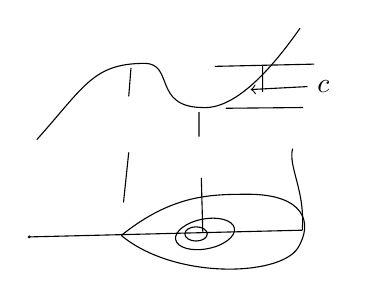
\begin{tikzpicture}[x=.95cm,y=.95cm]
\draw (.12,2.02) .. controls (.75,2.72) and (.87,3.04) .. (1.56,3.04)
      .. controls (1.96,3.04) and (1.67,2.46) .. (2.33,2.45)
      .. controls (2.75,2.42) and (3.22,2.91) .. (3.64,3.51);
\draw (2.50,3.00)--(3.83,3.03) (2.65,2.44)--(3.68,2.45)
      (3.14,3.01)--(3.14,2.66);
\draw[<-] (2.98,2.69)--(3.74,2.73) node[right] {$c$};
\draw (1.38,2.98)--(1.35,2.60) (2.29,2.39)--(2.29,2.06)
      (1.35,1.85)--(1.28,1.18) (2.32,1.51)--(2.34,.79)
      (3.54,1.90) .. controls (3.48,1.65) and (3.71,1.35) .. (3.67,.81);
\draw (.02,.72)--(3.67,.81);
\fill (.02,.72) circle (.021);
\draw (1.25,.74) .. controls (1.95,1.30) and (2.47,1.29) .. (2.98,1.29)
      .. controls (3.67,1.28) and (3.83,.93) .. (3.61,.57)
      .. controls (3.36,.19) and (1.96,.15) .. (1.25,.74);
\draw[rotate around={11:(2.37,.76)}] (2.37,.76) ellipse (.40 and .20);
\draw (2.25,.76) ellipse (.15 and .095);
\end{tikzpicture}}\endgroup}%
\par Тонкие вертикальные штрихи между кривыми местами прерываются.}
\end{GelfandAdjacentEvidence}
\begin{GelfandAdjacentEvidence}{GELFAND-P001201}{5}


$\dim\{I\}=n$ (счёт при пом. многогр. Ньютона\textsuperscript{?})
\Unclear{GELFAND-P001201}{newton-abbreviation}{многогр. Ньютона}
\end{GelfandAdjacentEvidence}
\begin{GelfandAdjacentEvidence}{GELFAND-P001201}{6}


(интегралы — ф-и от $c$; они обр. лин. пр-во; т.к. $\omega$ можно склад.)

\tikz{\node[draw,circle] {!};} \uwave{Утв.:} \uwave{число нулей}
$\overset{\text{любой рассм. ф-и}}{<n}$ (если она $\ne0$)

ф-и удовл. ур-ю Пикар--Фукса (связн. Гаусса--Манина)

\uwave{Комментарий:} $\forall f_1,\ldots,f_N$ комбин.
$c_1f_1+\cdots+c_Nf_N$ имеет $N-1$ нуль
(если лин. независ.)
\SourceFigure{GELFAND-P001201}{linear-combination-claim}{Написано «имеет $N-1$ нуль»; знака неравенства здесь нет.}
\end{GelfandAdjacentEvidence}
\begin{GelfandAdjacentEvidence}{GELFAND-P001201}{7}


Если число нулей $<\dim$, то сист. наз. \uwave{чебышевской}

(\uwave{неосцилляция})

\uwave{Вопрос:} связь с осцилл. теоремами?
\Unclear{GELFAND-P001201}{question-cancellation}{Под словом «Вопрос» заштрихована короткая черта; буквенное чтение не установлено.}
\end{GelfandAdjacentEvidence}
\begin{GelfandAdjacentEvidence}{GELFAND-P001201}{8}


\begin{center}--- \(\cdot\) ---\end{center}

\uwave{Счёт $\dim$}: $\int=0$ если а) полный диффер.

б) умн. чего-то на $H-c$.

\underline{Использование многогранника Ньютона для выч. размерностей}

\[
f=x^3+y^4;\qquad
\mathbb C[[x,y]]/(\tfrac{\partial f}{\partial x},\tfrac{\partial f}{\partial y})
\]

\SourceFigure{GELFAND-P001201}{newton-left-figure}{%
\par\smallskip
{\color{black}\begingroup\color{black}\GelfandFitDiagram{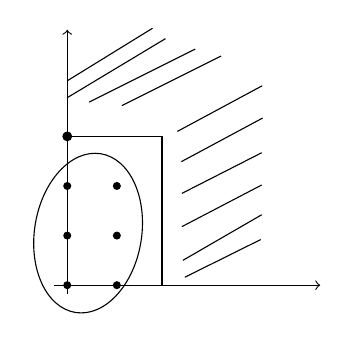
\begin{tikzpicture}[x=.63cm,y=.63cm]
\draw[->] (-.27,0)--(5.1,0);
\draw[->] (0,-.18)--(0,5.15);
\draw (0,3)--(1.91,3)--(1.91,0);
\draw (0,4.12)--(1.72,5.18) (0,3.78)--(1.98,4.97)
      (.44,3.69)--(2.58,4.76) (1.10,3.62)--(3.10,4.62)
      (2.22,3.10)--(3.93,4.02) (2.30,2.49)--(3.94,3.37)
      (2.31,1.85)--(3.92,2.67) (2.31,1.18)--(3.92,2.02)
      (2.33,.50)--(3.92,1.42) (2.37,.16)--(3.90,.92);
\foreach \x in {0,1}{\foreach \y in {0,1,2}{\fill (\x,\y) circle (.081);}}
\fill (0,3) circle (.10);
\draw[rotate around={-9:(.42,1.05)}] (.42,1.05) ellipse (1.08 and 1.62);
\end{tikzpicture}}\endgroup}}
\end{GelfandAdjacentEvidence}
\begin{GelfandAdjacentEvidence}{GELFAND-P001201}{9}


базис факторпр-ва. $\dim=6$

$x^2y+y^4$

\SourceFigure{GELFAND-P001201}{newton-right-figure}{%
\par\smallskip
{\color{black}\begingroup\color{black}\GelfandFitDiagram{\begin{tikzpicture}[x=.60cm,y=.60cm]
\draw (-.55,0)--(6.05,0) (0,-.06)--(0,3.32);
\draw (0,.41)--(.11,.48) (.64,-.05)--(.64,.08) (1.26,-.05)--(1.26,.06);
\draw (-.13,1.18) rectangle (.14,1.46) (1.77,-.14) rectangle (2.10,.13);
\draw (-.08,1.22)--(.06,1.41) (1.83,-.09)--(2.04,.07);
\draw (.64,1.35) circle (.14) (2.56,0) circle (.16);
\draw (.56,1.27)--(.65,1.45) (.65,1.26)--(.71,1.41)
      (2.46,-.10)--(2.53,.11) (2.55,-.11)--(2.62,.13) (2.63,-.07)--(2.68,.07);
\draw (.48,.56)--(.65,.80)--(.80,.57)--cycle;
\node[anchor=west] at (.20,-.69) {$\Rightarrow$ \uwave{базис}.};
\end{tikzpicture}}\endgroup}%
\par Внутренние штрихи в квадратах и кружках схематичны; их чтение не установлено.}
\end{GelfandAdjacentEvidence}



\Needspace{7\baselineskip}
\begin{GelfandAdjacentEvidence}{GELFAND-P001202}{1}
\SourcePage{GELFAND-P001202}{60}
\underline{А. Зелевинский.} О «самом красивом результате в обл. чистой мат.»

(Тройное тожд. Якоби)
\[
(1)\quad
\sum_{r=-\infty}^{\infty}z^r q^{r^2}
=\prod_{k=1}^{\infty}(1-q^{2k})(1+q^{2k-1}z)(1+q^{2k-1}z^{-1})
\]
(тройное тожд. Якоби)
\[
\Vert
\]
\[
(1;q^2)_\infty(-zq^{-1};q^2)_\infty(-z^{-1}q^{-1};q^2)_\infty
\]
\SourceFigure{GELFAND-P001202}{pochhammer-product}{В первом множителе перед точкой с запятой написано $1$. В двух следующих множителях написано $q^{-1}$.}
\end{GelfandAdjacentEvidence}
\begin{GelfandAdjacentEvidence}{GELFAND-P001202}{2}


Здесь
\[
(a;q)_\infty:=\prod_{n=0}^{\infty}(1-aq^n)
\]
!! Выводится из \uwave{тожд. Рамануджана.}

\uwave{Комбинаторное док-во}

Первое произв. перенесём в лев. часть
\[
(2)\quad
\left(\sum_{r=-\infty}^{\infty}z^r q^{r^2}\right)
\prod_{k=1}^{\infty}(1-q^{2k})^{-1}
=\prod_{k=1}^{\infty}(1+q^{2k-1}z)(1+q^{2k-1}z^{-1})
\]
\Unclear{GELFAND-P001202}{equation-two-cancellation}{В левой части (2) над $z^r$ густо зачёркнут знак.}
\end{GelfandAdjacentEvidence}
\begin{GelfandAdjacentEvidence}{GELFAND-P001202}{3}


Отличен от $0$ только коэфф. при $\underline{z^r q^{r^2+2n}}$

(и слева и справа)

$={}$ число разбиений числа $n$ на слаг. $=p(n)$

(слева)

(3) \uwave{Справа:} показатели
\[
\alpha_1>\alpha_2>\cdots>\alpha_s>0
\]
неч.
\[
\beta_1>\beta_2>\cdots>\beta_t>0
\]
\Unclear{GELFAND-P001202}{beta-inequalities}{Последний знак сравнения читается как $>$. Три предыдущих густо переправлены; чтение $>$ предположительное, возможно $\geq$.}
\end{GelfandAdjacentEvidence}
\begin{GelfandAdjacentEvidence}{GELFAND-P001202}{4}

\[
\sum\alpha_j+\sum\beta_i=r^2+2n,\qquad \underline{\underline{s-t=r}}
\]
[От «неч.» два расходящихся штриха к строкам $\alpha$ и $\beta$; по сторонам строк проведены вертикальные разделители.]

\SourceFigure{GELFAND-P001202}{both-descriptions}{И то и другой}
\end{GelfandAdjacentEvidence}
\begin{GelfandAdjacentEvidence}{GELFAND-P001202}{5}

(З.Л. Лейбензон) --- комбинат. описание мн-ва:
\SourceFigure{GELFAND-P001202}{leibenzon-name}{З.Л. Лейбензон}
\end{GelfandAdjacentEvidence}
\begin{GelfandAdjacentEvidence}{GELFAND-P001202}{6}

\[
00000\,1\,0000\,1\,00\,111111
\]
беск. слова (\uwave{сцепления})

[Зачёркнуто: слева\textsuperscript{?}]
\Unclear{GELFAND-P001202}{cancelled-left-word}{слева}
\end{GelfandAdjacentEvidence}

снач. беск. число $0$; потом каша; потом \underline{палочки}

(беск. число)

Высота: $h(A)$ --- число инверсий $\underbrace{1\,0}$ --- как угодно далеко друг от друга

$\underline{h(A)=n}\quad\Rightarrow$ число элем. $p(n)$

--- параметриз. наборами вида (3).

\underline{1-й способ}
\[
0000\,1\,0\,111\qquad\text{--- выс. }1
\]
$p(n)$ --- возьмём лев. палочку, счит. за ней нули и т.д.

\underline{2-й способ}

Пробелы имеют [над «номер»: (естеств.)] номер:
(число $1$ слева) $-$ (число $0$ справа)

\uwave{Номер} мен. от $-\infty$ до $+\infty$ !! (всюду!)


\Needspace{7\baselineskip}
\begin{GelfandAdjacentEvidence}{GELFAND-P001203}{1}
\SourcePage{GELFAND-P001203}{unlabelled}
\uwave{Замет. Арнольда:}

Изобразим:

$0$ --- ход вправо

$1$ --- ход вверх

\SourceFigure{GELFAND-P001203}{young-step-diagram}{%
\par\smallskip
{\color{black}\begingroup\color{black}\GelfandFitDiagram{\begin{tikzpicture}[x=.48cm,y=.38cm]
\draw (-4.5,0)--(0,0)--(0,1)--(2,1)--(2,2)--(3,2)--(3,4)--(4,4)--(4,7.3);
\draw[line width=1.4pt] (3,4)--(4,4);
\node at (-.35,-.42) {$0$};
\node at (-.27,.50) {$1$};
\node at (.50,1.40) {$0$};
\node at (1.50,1.40) {$0$};
\node at (2.30,1.55) {$1$};
\node at (2.52,2.44) {$0$};
\node at (3.32,2.53) {$1$};
\node at (3.32,3.53) {$1$};
\node at (3.50,4.44) {$0$};
\node at (4.32,4.59) {$1$};
\node at (4.32,5.59) {$1$};
\node at (4.32,6.63) {$1$};
\end{tikzpicture}}\endgroup}}
\end{GelfandAdjacentEvidence}
\begin{GelfandAdjacentEvidence}{GELFAND-P001203}{2}


диагр. Юнга

ф-я $\underline{x-y}$ \uwave{нумерует} все

Рассм. пробел с номером $r$.

Сцепление характеризуем так:

расст. от пробела до палочек, \textit{[под словом с фигурным указателем: леж. слева]} $\Vert$ \uwave{нечётные числа}.

--- ″ --- кружочков. \textit{[под словом с фигурным указателем: леж. справа]}
\[
\sum\alpha_j+\sum\beta_j=r^2+2n
\]
из площади под кривой.

\Needspace{7\baselineskip}
16/IX--85 г. \underline{Сем. Гельфанда.}

\underline{Зелевинский} (\underline{и Бейлинсон}) со слов \uwave{M.-F. Vigneras} (Marie-France Vigneras)
\Unclear{GELFAND-P001203}{name-aside}{Над «to» приписка в скобках, предположительно «Ma’tici». После a виден отдельный верхний штрих.}
\end{GelfandAdjacentEvidence}
\begin{GelfandAdjacentEvidence}{GELFAND-P001203}{3}


1) о раб. «From \(\mathrm{GL}(2,\mathbb Q\sqrt d)\) to \(\mathrm{GSp}(4,\mathbb Q)\)» (M.-F. Vigneras)
\Unclear{GELFAND-P001203}{lifting-field-notation}{Первая буква в обозначении поля переправлена; читается как \(\mathbb Q\sqrt d\).}
\end{GelfandAdjacentEvidence}
\begin{GelfandAdjacentEvidence}{GELFAND-P001203}{4}


Стр. соотв. между представлениями.

(лифтинг)

При переходе к $p$-адич. полю

это позволяет проверить для \(\mathrm{GSp}(4,F)\) какую-то гипотезу Ленглендса о функториальности.

\textit{[Справа, с указателем к \(\mathrm{GSp}\):]} симплект. подобия (сохр. симпл. форму с точн. до множителя)

\textit{[Под \(F\):]} $p$-адич.

2) \uwave{Rallis, Пятецкий--Шапиро и др.}
\[
L(s,\pi_1\times\pi_2\times\pi_3),\quad
\text{где }\pi_j\text{ --- предст. }\mathrm{GL}_2(F)
\]
3) По рассказу Jacket «\underline{Как} \underline{использовать} ф-лу следа?»
\SourceFigure{GELFAND-P001203}{latin-surname}{Фамилия в рукописи читается как «Jacket».}
\end{GelfandAdjacentEvidence}
\begin{GelfandAdjacentEvidence}{GELFAND-P001203}{5}


Посл. важный результат --- теор. Пэли--Винера,
\Unclear{GELFAND-P001203}{cancelled-theorem-phrase}{Предположительное начало зачёркнутых слов после названия теоремы: «об \ldots».}
\end{GelfandAdjacentEvidence}
\begin{GelfandAdjacentEvidence}{GELFAND-P001203}{6}

док. Кажданом и Бернштейном.

\SourceFigure{GELFAND-P001203}{result-abbreviation}{Сокращение в начале строки читается как «Посл.».}
\end{GelfandAdjacentEvidence}
\begin{GelfandAdjacentEvidence}{GELFAND-P001203}{7}


\textit{[В овале, с указателем к названию результата:]} о предст. над \(F\)

\(G\) --- редукт. $p$-адич. гр. (напр. \(\mathrm{GL}_n\))

\(H^{\bullet}(G)\) --- [Вписано над тире: алг.] лок. пост. финитных ф-й на \(G\).
\SourceFigure{GELFAND-P001203}{hecke-superscript}{Надстрочный знак после \(H\) читается как точка.}
\end{GelfandAdjacentEvidence}
\begin{GelfandAdjacentEvidence}{GELFAND-P001203}{8}

\SourceFigure{GELFAND-P001203}{algebra-insertion}{Над тире вписано «алг.»; фигурный штрих связывает вставку со строкой.}
\end{GelfandAdjacentEvidence}
\begin{GelfandAdjacentEvidence}{GELFAND-P001203}{9}


\textit{[Справа от вертикального штриха:]} лок. пост. заменяют \(C^\infty\)-ф-и

По \(f\) строим:
\[
\pi\longrightarrow\operatorname{tr}\pi(f)
\]
--- функцию на \(\operatorname{Irr}G\)

Здесь
\[
\pi(f)=\int_G f(g)\pi(g)\,dg
\]
\underline{Теорема} (Пэли--Винера по К.-Б.) даёт описание всех таких ф-й

Непр. предст. делятся на листы и сем-ва: по \(\rho\in\operatorname{Irr}M\) строится

\(M\subset G\)
\[
\pi\in\mathrm{JH}\;\operatorname{Ind}_{\underline{P}}^{G}\rho
\]
(ряд Жорд.--Гельдера)
\Unclear{GELFAND-P001203}{induction-subscript}{Под нижним индексом видна черта. Переправленная буква предположительно читается как \(P\).}
\end{GelfandAdjacentEvidence}
\begin{GelfandAdjacentEvidence}{GELFAND-P001203}{10}


\(\Vert\) каждое сем-во приобрет. структуру

\(M\) --- подгр. Леви параб. подгруппы в \(G\)

(полупр. часть)

характер непр. предст. \(\Leftrightarrow\) \underline{алгебраичность} нек-рой ф-и

Идея в вещ. \textit{[под «вещ.» в обводке: и компл.?]} случае: убыв.\textsuperscript{?} на \(\forall\) картановской подалгебре
\Unclear{GELFAND-P001203}{final-verb}{Возможны чтения «убыв.» и «убив.».}
\end{GelfandAdjacentEvidence}



\Needspace{7\baselineskip}
\begin{GelfandAdjacentEvidence}{GELFAND-P001204}{1}
\SourcePage{GELFAND-P001204}{61}
\underline{M.-F. Vigneras.}\quad (об этом же, но более точн.)
\Unclear{GELFAND-P001204}{upper-aside-final}{В конце приписки читается «точн.»; последняя буква перед скобкой не вполне различима.}
\end{GelfandAdjacentEvidence}
\begin{GelfandAdjacentEvidence}{GELFAND-P001204}{2}


\(G\) reductive \(p\)-adic group (напр., \(\mathrm{GL}_n\))
\begin{equation*}
\coprod_{(M,\rho)}\{\rho\chi\}^{W}=\operatorname{Irr}G \tag{1}
\end{equation*}
\textit{[Подписи с выносными линиями:]} \(M\) --- станд. ред. подгр.,
\(\rho\) --- неприв. куспидальное предст.,
\(\chi\) --- неразветвл. характер,
\(W\) --- с точн. до действия гр. Вейля.
\SourceFigure{GELFAND-P001204}{upper-m-caption}{Первая строка подписи к \(M\) читается как «станд.».}
\end{GelfandAdjacentEvidence}
\begin{GelfandAdjacentEvidence}{GELFAND-P001204}{3}


\(\{\rho\chi\}^{W}\) --- конечномерное алг. мн-же (\(\text{над }\mathbb C\)).

по \(f\in H(G)\) стр. ф-я на [вставлено: мн-ве (1)]
\[
\pi\longrightarrow\operatorname{trace}\operatorname{ind}_{M}^{G}\rho\chi(f)
\]
Условия

а) алгебраична на \(\forall\) таком мн-жии

б) сосредот. на их конечном числе

\Needspace{6\baselineskip}
\underline{\underline{Бейлинсон.}}
\Unclear{GELFAND-P001204}{middle-beilinson-cancel}{Слова под заголовком зачёркнуты, точное чтение не установлено.}
\end{GelfandAdjacentEvidence}
\begin{GelfandAdjacentEvidence}{GELFAND-P001204}{4}


Предст. \(\mathrm{GSp}(4,\mathbb Q)\) --- ?
\[
W_{\mathbb Q_p}\subset\operatorname{Gal}(\overline{\mathbb Q}_p/\mathbb Q_p)
\]
\[
\operatorname{Irr}\mathrm{GSp}(4,\mathbb Q)
\longrightarrow \text{предст. гр. Вейля--Делиня}
\]
\Unclear{GELFAND-P001204}{middle-wd-sign}{После стрелки, перед «предст.», густо переправлен знак. Его чтение и роль не установлены.}
\end{GelfandAdjacentEvidence}
\begin{GelfandAdjacentEvidence}{GELFAND-P001204}{5}


\textit{[С выносной линией к правой части стрелки:]} прообр. \(\forall\) точки конечен (\(L\)-пакет)
\[
\mathrm{GL}(2,\mathbb Q(\sqrt d))\longrightarrow\mathrm{GO}(4)
\]
\[
\left\{x\in M(2,\mathbb Q(\sqrt d)):x=\bar x\right\}
\qquad
x=\begin{pmatrix}a&b\\\bar b&d\end{pmatrix}
\]
\SourceFigure{GELFAND-P001204}{middle-hermitian-condition}{В условии читается \(x=\bar x\); знак транспонирования не виден.}
\end{GelfandAdjacentEvidence}
\begin{GelfandAdjacentEvidence}{GELFAND-P001204}{6}


\(\det\) --- кан. квадр. форма\quad (он рационален)
\[
x\longmapsto gx\bar g^{t}\qquad\text{сохр. это условие}
\]
(аналог спинорного предст.)

Предст. Вейля: предст. \(\mathrm{GO}(4)\times\mathrm{GSp}(4)\)

оно реализуется в \(\theta\)-ф-ях

\Needspace{6\baselineskip}
\underline{\underline{Б. Фейгин.}}\qquad \underline{О струнах}
\Unclear{GELFAND-P001204}{lower-theory-cancel}{Зачёркнутое слово перед «Теория струн» не разобрано.}
\end{GelfandAdjacentEvidence}
\begin{GelfandAdjacentEvidence}{GELFAND-P001204}{7}


Теория струн --- статистика поверхностей.

Квант. мех. изучает пр-во с лагранжианом; действие зав. от траектории.

Струны: вместо траектории --- поверхность.

\(\mathcal E\) --- риманова пов., рассм. пр-во \(\mathbb R^d\)

Траект. --- отобр.
\[
\underset{x_1,\ldots,x_d}{\{\mathcal E\longrightarrow\mathbb R^d\}}.
\]
\uwave{Идея:} все элем. част. опис. отображениями \(\mathcal E\) в суперпр-во \(\mathbb R^{10/m}\)
\SourceFigure{GELFAND-P001204}{string-super-dimension}{В показателе видны наклонная черта и \(m\): \(10/m\).}
\end{GelfandAdjacentEvidence}
\begin{GelfandAdjacentEvidence}{GELFAND-P001204}{8}


Движ. окружности --- поверхность
\SourceFigure{GELFAND-P001204}{circle-worldsheet}{%
\par\smallskip
{\color{black}\begingroup\color{black}\GelfandFitDiagram{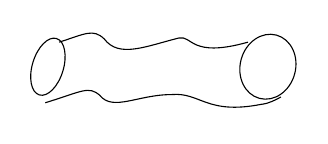
\begin{tikzpicture}[x=1.1cm,y=1.04cm]
\draw[rotate around={-17:(0,0)}] (0,0) ellipse (.18 and .36);
\draw[rotate around={-15:(2.54,0)}] (2.54,0) ellipse (.32 and .40);
\draw (.13,.30) .. controls (.43,.40) and (.52,.47) .. (.65,.34)
 .. controls (.82,.10) and (1.13,.25) .. (1.51,.35)
 .. controls (1.67,.39) and (1.64,.10) .. (2.31,.30);
\draw (-.03,-.44) .. controls (.40,-.30) and (.47,-.23) .. (.60,-.35)
 .. controls (.75,-.55) and (1.04,-.34) .. (1.43,-.34)
 .. controls (1.76,-.31) and (1.83,-.59) .. (2.46,-.46)
 .. controls (2.55,-.45) and (2.62,-.41) .. (2.69,-.37);
\end{tikzpicture}}\endgroup}}
\end{GelfandAdjacentEvidence}


Класс. аналог --- рост кристалла.


\Needspace{7\baselineskip}
\begin{GelfandAdjacentEvidence}{GELFAND-P001205}{1}
\SourcePage{GELFAND-P001205}{unlabelled}
Лагранжиан:
\begin{equation*}
\mathcal L=\int\text{[зачёркнуто]}\,
(\det g_{ij})^{1/2}\,d\sigma\,d\tau
\qquad \text{(лагранжиан Намбу)} \tag{1}
\end{equation*}
\Unclear{GELFAND-P001205}{upper-lagrangian-cancel}{Сразу после знака интеграла зачёркнут фрагмент, точное чтение не установлено.}
\end{GelfandAdjacentEvidence}
\begin{GelfandAdjacentEvidence}{GELFAND-P001205}{2}

(площадь в индуц. метрике)

Надо рассм. фейнмановский интеграл.
\[
X:\mathcal E\hookrightarrow\mathbb R^d
\]
Другая запись (1):
\begin{equation*}
\mathcal L(X)=\int d\sigma\,d\tau
\left[
\left(\frac{\partial X}{\partial\sigma}\right)^2
\left(\frac{\partial X}{\partial\tau}\right)^2
-\left(\frac{\partial X}{\partial\sigma}\cdot
\frac{\partial X}{\partial\tau}\right)^2
\right]^{1/2} \tag{1'}
\end{equation*}
Фейнман. интеграл
\begin{equation*}
\int e^{\beta\mathcal L(X)}\,\mathcal D X \tag{2}
\end{equation*}
Есть 2 подхода: через интегр. и через обычные операторы (!) и теперь установлено соответствие.

\Needspace{7\baselineskip}
\uwave{Поляков:} другой контин. интеграл

\(\widetilde X\) --- [вставлено: пр-во] элементы к-рого --- пары

1) \(X:\mathcal E\longrightarrow\mathbb R^d\)

2) \(g_{ij}\) на \(\mathcal E\) (рим. метрика на \(\mathcal E\))

Лагранжиан Полякова:
\begin{equation*}
\text{[зачёркнуто]}\,
\mathcal L=\text{\ae}\int(\det g_{ij})^{1/2}
+\int\frac{\partial X_i}{\partial\xi_\alpha}
\frac{\partial X_i}{\partial\xi_\beta}g^{\alpha\beta}
\overset{\text{[вставлено]}}{\sqrt g}\,d\xi_1\,d\xi_2
\tag{3}
\end{equation*}
\Unclear{GELFAND-P001205}{lower-lagrangian-cancel}{Перед \(\mathcal L\) зачёркнут знак, точное чтение не установлено.}
\end{GelfandAdjacentEvidence}
\begin{GelfandAdjacentEvidence}{GELFAND-P001205}{3}

\Unclear{GELFAND-P001205}{lower-lagrangian-coefficient}{Коэффициент перед первым интегралом передан знаком формы «æ». Точное чтение знака не установлено.}
\end{GelfandAdjacentEvidence}
\begin{GelfandAdjacentEvidence}{GELFAND-P001205}{4}

\SourceFigure{GELFAND-P001205}{polyakov-measure}{\(\sqrt g\) вставлено над строкой. Переправленные нижние индексы в \(d\xi_1\,d\xi_2\) читаются как \(1,2\).}
\end{GelfandAdjacentEvidence}


[Вставлено: К нему] Применима техника вычисления

Способ работы: фиксируем \(g_{ij}\) и вычисляем интеграл по \(X\) --- он квадратичный.
\begin{center}--- \(\cdot\) ---\end{center}


\Needspace{7\baselineskip}
\begin{GelfandAdjacentEvidence}{GELFAND-P001206}{1}
\SourcePage{GELFAND-P001206}{62}
\underline{23.9.85 г.}\quad\underline{Сем. Гельфанда.}

\uwave{И.М.Г.} \underline{Задача (для 9 кл.)}
Какой многогранник получается в сечении 4-мерного куба 3-мерной гиперплоскостью, проходящей через центр и перпендикулярной главной диагонали?

\underline{А. Бейлинсон.} \uwave{О новой серии раб. Пятецкого--Шапиро и Раллиса.}

функц. ур-я $L$-ф-и, связ. с автом. формами

\(G\) --- полупр. группа над \(\mathbb Q\) (напр., гр. матриц \(n\times n\))

\(G/\mathbb Q\).
\Unclear{GELFAND-P001206}{upper-gq-cancel}{Знаки справа от \(G/\mathbb Q\) густо зачёркнуты.}
\end{GelfandAdjacentEvidence}
\begin{GelfandAdjacentEvidence}{GELFAND-P001206}{2}


\underline{Задача:} описать представления адельной группы \(G(A)\) в \(L^2(G(A)/G(\mathbb Q)\)
\SourceFigure{GELFAND-P001206}{upper-l2-parentheses}{В записи пространства \(L^2\) видна одна закрывающая скобка после \(\mathbb Q\).}
\end{GelfandAdjacentEvidence}
\begin{GelfandAdjacentEvidence}{GELFAND-P001206}{3}


Соотв. представл. наз. \uwave{автоморфными}.
\begin{center}--- \(\cdot\) ---\end{center}
\uwave{И.М.Г.} \(\forall\) нат. число запис. в виде
\[
a_0+a_1p+a_2p^2+\ldots+a_np^n
\]
Всякое рац. число
\[
a_{-m}p^{-m}+a_1p^{-m+1}+\ldots+a_kp^k+
\]
\SourceFigure{GELFAND-P001206}{middle-rational-expansion}{Во втором слагаемом читается \(a_1p^{-m+1}\). После \(a_kp^k\) стоит знак \(+\).}
\end{GelfandAdjacentEvidence}
\begin{GelfandAdjacentEvidence}{GELFAND-P001206}{4}


Например,
\[
\frac13=1+1\cdot2+1\cdot2^3+1\cdot2^5+\ldots
\]
\textit{[Справа:]}
\[
\|a\|=p^{-n},\quad\text{если }a=p^nm,\quad(a,m)=1.
\]
\SourceFigure{GELFAND-P001206}{middle-coprimality}{Условие взаимной простоты читается как \((a,m)=1\).}
\end{GelfandAdjacentEvidence}
\begin{GelfandAdjacentEvidence}{GELFAND-P001206}{5}

\[
\underline{p=2}\quad\Rightarrow\quad
\|2\|=\frac12;\quad\|3\|=1,\quad\|4\|=\frac14,\quad
\left\|\frac12\right\|=2.
\]
\[
\text{Адели}=\prod_p(\text{\(p\)-адич. чисел})
\]
\SourceFigure{GELFAND-P001206}{middle-adeles-product}{В рукописи «\(p\)-адич. чисел»; под знаком произведения стоит \(p\).}
\end{GelfandAdjacentEvidence}
\begin{GelfandAdjacentEvidence}{GELFAND-P001206}{6}

\begin{center}--- \(\cdot\) ---\end{center}
\[
\mathrm{SL}_2(\mathbb R)\supset\mathrm{SL}_2(\mathbb Z)\supset\Gamma_n
\]
\textit{[Выносная подпись к \(\Gamma_n\):]} матр. 2-го пор.,
[зачёркнуто: элем.?] к-рые сравн-мы\textsuperscript{?} с \(1\) (матр.) \(\bmod n\).
\Unclear{GELFAND-P001206}{middle-matrices-cancel}{Зачёркнутое сокращение после «пор.» предположительно читается как «элем.».}
\end{GelfandAdjacentEvidence}
\begin{GelfandAdjacentEvidence}{GELFAND-P001206}{7}

\Unclear{GELFAND-P001206}{middle-matrices-congruence}{Видно «сравн»; переправленный конец слова предположительно читается как «-мы».}
\end{GelfandAdjacentEvidence}
\begin{GelfandAdjacentEvidence}{GELFAND-P001206}{8}

\[
\Gamma_{n_1}\supset\Gamma_{n_2}\quad\text{при }n_1\mid n_2
\]
\[
G(A)/G(\mathbb Q)=\varprojlim_n G(\mathbb R)/\Gamma_n.
\]
\(\Gamma_n\) действ. на верхн. полупл. \(H\); \(H/\Gamma_n\) ---
[зачёркнуто: риманова?] [вставлено: сфера] (с выкол. точками)
\Unclear{GELFAND-P001206}{lower-surface-cancel}{Первое зачёркнутое слово предположительно «риманова». Над строкой вписано «сфера».}
\end{GelfandAdjacentEvidence}
\begin{GelfandAdjacentEvidence}{GELFAND-P001206}{9}


\(H/\mathrm{SL}_2(\mathbb Z)\) --- сфера с 2-мя проколами

\(H/\Gamma_2\) --- --- ″ --- 3-мя проколами
\SourceFigure{GELFAND-P001206}{lower-modular-quotients}{В первой строке написано «сфера с 2-мя проколами».}
\end{GelfandAdjacentEvidence}
\begin{GelfandAdjacentEvidence}{GELFAND-P001206}{10}

\[
\pi_{G(A)}=\pi_{G(\mathbb R)}\otimes\pi_{G(\mathbb Q_2)}\otimes\ldots
\]
\begin{center}--- \(\cdot\) ---\end{center}
\uwave{И.М.Г.} На \uwave{Sem. Bourbaki} есть раб. \uwave{A. Connes}
\underline{о связи топ. узлов с инвариантами факторов}!!
\SourceFigure{GELFAND-P001206}{lower-knot-abbreviation}{Сокращение перед словом «узлов» читается как «топ.».}
\end{GelfandAdjacentEvidence}
\begin{GelfandAdjacentEvidence}{GELFAND-P001206}{11}

\begin{center}--- \(\cdot\) ---\end{center}
Дост. знать предст. $p$-адич. группы.
\Unclear{GELFAND-P001206}{lower-padic-cancel}{Зачёркнутый знак в конце строки не разобран.}
\end{GelfandAdjacentEvidence}
\begin{GelfandAdjacentEvidence}{GELFAND-P001206}{12}


Какие встречаются в \(L^2(G(A)/G(\mathbb Q))\)? Далеко не все.

\uwave{Представления} \(G(\mathbb Q_p)\).

Простейшие --- сферические, когда есть вектор, инв. отн. [вставлено: max] компактной подгр.
\[
G(\mathbb Q_p)/B(\mathbb Q_p)
\]
\SourceFigure{GELFAND-P001206}{borel-matrix-layout}{%
\par\smallskip
{\color{black}\(\displaystyle B=
\begin{pmatrix}
\ast&&&\\[-.45em]
&\ast&&\\[-.45em]
0&&\ast&\\[-.45em]
&&&\ast
\end{pmatrix}\)}}
\end{GelfandAdjacentEvidence}



\Needspace{7\baselineskip}
\begin{GelfandAdjacentEvidence}{GELFAND-P001207}{1}
\SourcePage{GELFAND-P001207}{unlabelled}

нумеруются неразветвл. хар-рами тора \(\chi_{nr}(T)\)
\(=\) точки двойств. тора \(=T^0(\mathbb C)\) (компл. точки)
\Unclear{GELFAND-P001207}{top-character-subscript}{Нижний индекс при \(\chi\) предположительно читается как \(nr\); второй знак не вполне ясен.}
\end{GelfandAdjacentEvidence}
\begin{GelfandAdjacentEvidence}{GELFAND-P001207}{2}


(трив. на пересеч. тора с \(\max\) комп. подгр.)

Сферич. предст. \(G(\mathbb Q_p)=T^0(\mathbb C)/W\)

неразветвл. хар. \(\longrightarrow\) класс сопряжённости в гр. матриц

\begin{center}--- \(\cdot\) ---\end{center}

Пусть \(G\) --- расщепленная группа (\(\max\) тор расщепляется)

\(G^0\) --- двойств. группа\qquad (\(G=\mathrm{GL}\Rightarrow G^0=\mathrm{GL}\))

\SourceFigure{GELFAND-P001207}{satake-parameter-diagram}{%
\par\smallskip
{\color{black}\begingroup\color{black}\GelfandFitDiagram{\begin{tikzpicture}[x=.78cm,y=.78cm]
\node at (2.00,1.45) {\(\rho:\)};
\node at (2.79,1.45) {\(G^0\)};
\node at (3.97,1.45) {\(\longrightarrow\)};
\node at (5.91,1.45) {\(\mathrm{GL}(m,\mathbb C)\)};
\node[rotate=90] at (2.79,.70) {\(\in\)};
\node at (.0,0) {\(\pi_{\mathbb Q_p}\)};
\node at (1.17,0) {\(\rightsquigarrow\)};
\node at (2.79,0) {\(x\)};
\node at (3.97,0) {\(\longmapsto\)};
\node at (6.05,0) {\(\det(1-t\rho(x))\)};
\node[align=center,text width=2.0cm,font=\small] at (.0,-.78) {сфер. предст.};
\node[align=center,text width=2.9cm,font=\small] at (6.05,-.78) {хар. многочлен};
\end{tikzpicture}}\endgroup}}
\end{GelfandAdjacentEvidence}
\begin{GelfandAdjacentEvidence}{GELFAND-P001207}{3}


Пусть для \(\pi_{G(A)}\) почти все предст.
[Вписано над строкой: (лок. группы \(G(\mathbb Q_p)\))] сферические
(все кроме конечн. числа)

\[
L(\pi,\rho,s)=\prod_p
\frac{1}{\det\left(1-p^{-s}\rho\left(
\underset{\substack{\vert\\\text{полупростой элем.}}}{x_{\pi_{\mathbb Q_p}}}
\right)\right)}
\]

\begin{center}--- \(\cdot\) ---\end{center}

\underline{Пример}.
\[
\rho:\mathrm{GL}_1\underset{\text{един.}}{\longrightarrow}\mathrm{GL}_1
\quad\Rightarrow\quad
x\longmapsto\underset{\text{многоч.\textsuperscript{?}}}{1-tx}
\]
\Unclear{GELFAND-P001207}{example-polynomial-caption}{Под \(1-tx\) сокращение предположительно читается как «многоч.» или «многочл.».}
\end{GelfandAdjacentEvidence}
\begin{GelfandAdjacentEvidence}{GELFAND-P001207}{4}

\Unclear{GELFAND-P001207}{example-cancelled-symbol}{Зачёркнутый знак перед \(x=1\) не разобран.}
\end{GelfandAdjacentEvidence}
\begin{GelfandAdjacentEvidence}{GELFAND-P001207}{5}


\(x=1\Rightarrow L(\pi,\rho,s)=\prod_p\frac{1}{1-p^{-s}}\)
--- \(\zeta\)-ф-я Римана.

\Needspace{7\baselineskip}
\underline{\underline{Фейгин Б.}}\qquad\underline{О струнах (продолжение).}

\(\mathcal E\) --- риманова пов. (2-мерное мн-зие);
\(\mathbb R^d\) --- пр-во с метрикой Минковского
\(\langle\, , \,\rangle\) (1 отр. квадр.) или евклидовой.

Рассм. пр-во [Вписано над строкой: \(X\)] гладких отбр.
\(\mathcal E\overset{x}{\longrightarrow}\mathbb R^d\)

[Вписано над строкой: Отобр. \(x\) индуцирует]
на \(\mathcal E\) [зачёркнуто] рим. метрика.
\Unclear{GELFAND-P001207}{metric-cancelled-word}{Зачёркнутое слово после \(\mathcal E\) предположительно начинается «зад…».}
\end{GelfandAdjacentEvidence}
\begin{GelfandAdjacentEvidence}{GELFAND-P001207}{6}


Пусть \(\xi_1,\xi_2\) --- координаты [зачёркнуто] на \(\mathcal E\).
\Unclear{GELFAND-P001207}{coordinates-cancelled-symbol}{Зачёркнутая запись между «координаты» и «на» не разобрана.}
\end{GelfandAdjacentEvidence}

\begin{equation*}
g_{ij}=\left(\frac{\partial x}{\partial\xi_i},
\frac{\partial x}{\partial\xi_j}\right)
\qquad \{g^{ij}\}=\{g_{ij}\}^{-1}
\tag{1}
\end{equation*}
Лагранжиан Намбу:
\begin{equation*}
\mathcal L(x)=\int_{\mathcal E}\omega
=\int_{\mathcal E}\sqrt g\,d\xi_1\,d\xi_2,
\qquad g=\det\{g_{ij}\}
\tag{2}
\end{equation*}
(площ. пов. в рим. метрике)


\Needspace{7\baselineskip}
\begin{GelfandAdjacentEvidence}{GELFAND-P001208}{1}
\SourcePage{GELFAND-P001208}{63}

Континуальный интеграл
\begin{equation*}
\int e^{\frac{i}{h}\mathcal L(x)}\mathcal D x
\tag{3}
\end{equation*}
\Unclear{GELFAND-P001208}{exponential-coefficient}{Коэффициент переправлен; предположительное чтение \(i/h\). Зачёркнутый знак слева не разобран.}
\end{GelfandAdjacentEvidence}
\begin{GelfandAdjacentEvidence}{GELFAND-P001208}{2}


По всем поверхн., прох. через зад. точки [зачёркнуто] и т.п. (будет уточнено ниже).
\Unclear{GELFAND-P001208}{surfaces-cancelled-word}{Зачёркнутое слово после «точки» не разобрано.}
\end{GelfandAdjacentEvidence}
\begin{GelfandAdjacentEvidence}{GELFAND-P001208}{3}


Хотим найти [зачёркнуто] \(\min\) лагранжиана \(\mathcal L\).
\Unclear{GELFAND-P001208}{minimum-cancelled-symbol}{Зачёркнутый знак перед \(\min\) не разобран.}
\end{GelfandAdjacentEvidence}

Это минимальная поверхность.

\uwave{Св-ва \(\min\) поверхностей.}

а) \(\mathcal L\) не зав. от выбора координат.

\uwave{Вариация \(\mathcal L\).}

Пусть задано 1-пар. сем-во \(x(t)\) таких поверхностей.
\begin{equation*}
\left.\frac{\partial\mathcal L}{\partial t}\right|_{t=0}
=-\int(\dot{x}_t,H)\sqrt g\,d\xi_1\,d\xi_2.
\tag{4}
\end{equation*}

Здесь
\[
H=\Delta x=\frac{1}{\sqrt g}\sum_i\frac{\partial}{\partial\xi_i}
\left(\sqrt g\sum_j g^{ij}\frac{\partial x}{\partial\xi_j}\right)
\]
(опер. Лапласа метрики)

(5)\quad\underline{Следствие:}

\uwave{если \(x:\mathcal E\longrightarrow\mathbb R^d\) задаётся гармоническими ф-ями, то пов. минимальна.}

\begin{center}--- \(\cdot\) ---\end{center}

\underline{И.М.Г.}\quad \uwave{Иллс} заним. мин. пов.

\uwave{Лашоф}\quad --- ″ ------; к-рые стр. по группам.

\begin{GelfandAdjacentEvidence}{GELFAND-P001208}{4}
Пусть;
\begin{equation*}
x:\mathcal E\longrightarrow\mathbb R^d;
\qquad\underline{\Delta x=0};\qquad\text{тогда}
\tag{6}
\end{equation*}

[зачёркнуто: Пусть задана] [Вписано над строкой: Для]
вар. \(\delta x\) и сем-ва \(x+t\delta x\) 2-я вар. имеет вид
\begin{equation*}
\left.\frac{\partial^2\mathcal L}{\partial t^2}\right|_{t=0}
=-\int(\Delta\delta x,\delta x)\sqrt g\,d\xi_1\,d\xi_2
\tag{7}
\end{equation*}
\Unclear{GELFAND-P001208}{second-variation-hypotheses}{В числителе знак \(\partial\) переправлен. Условие \(\Delta x=0\) записано выше, в (6).}
\end{GelfandAdjacentEvidence}
\begin{GelfandAdjacentEvidence}{GELFAND-P001208}{5}


Получим тогда
\begin{equation*}
\mathcal L(x+\delta x)=\mathcal L(x)-
\underbrace{\int(\Delta\delta x,\delta x)\sqrt g\,d\xi_1\,d\xi_2}_{
\substack{\text{лагранжиан свободного поля}\\\text{на этой пов.}}}
+O(\delta x^2)
\tag{8}
\end{equation*}
\SourceFigure{GELFAND-P001208}{second-variation-expansion}{В рукописи перед интегралом нет множителя \(1/2\); остаток записан \(O(\delta x^2)\).}
\end{GelfandAdjacentEvidence}
\begin{GelfandAdjacentEvidence}{GELFAND-P001208}{6}


Теперь метрика \(g_{ij}\) фиксирована на \(\mathcal E\).
Заменяя \(\delta x\) на \(x\), запишем лагр. своб. поля в виде.
\SourceFigure{GELFAND-P001208}{free-field-form-word}{Перед словом «виде» виден нижний штрих индекса \(j\) из строки выше. В строке написано «в виде».}
\end{GelfandAdjacentEvidence}
\begin{GelfandAdjacentEvidence}{GELFAND-P001208}{7}


\begin{equation*}
\mathcal L=\int\left(\frac{\partial x}{\partial\xi_i},
\frac{\partial x}{\partial\xi_j}\right)g^{ij}\sqrt g\,d\xi_1\,d\xi_2
\tag{9}
\end{equation*}

(10)\quad \uwave{Экстремали --- такие} \(x\), что \(\Delta x=0\).

(11)\quad \uwave{тогда индуц. метрика будет конформно эквивалентна [Вписано над строкой: исходной] метрике \(g_{ij}\).}
\SourceFigure{GELFAND-P001208}{lower-claim-opening}{Начало подчёркнутой строки читается как «Тогда».}
\end{GelfandAdjacentEvidence}
\begin{GelfandAdjacentEvidence}{GELFAND-P001208}{8}

\SourceFigure{GELFAND-P001208}{induced-metric-conformality}{«Исходной» вписано над строкой, перед словом «метрике».}
\end{GelfandAdjacentEvidence}



\Needspace{7\baselineskip}
\begin{GelfandAdjacentEvidence}{GELFAND-P001209}{1}
\SourcePage{GELFAND-P001209}{unlabelled}
Перепишем:
\begin{equation*}
\mathcal L(x,g_{ij})=
\int\left(\frac{\partial x}{\partial\xi_i},\frac{\partial x}{\partial\xi_j}\right)
g^{ij}\sqrt g\,d\xi_1\,d\xi_2 \tag{9'}
\end{equation*}
Рассмотрим конт. интеграл
\begin{equation*}
\int e^{ih^{-1}\mathcal L(x,g_{ij})}\mathcal D x\,\mathcal D g_{ij}. \tag{12}
\end{equation*}
Теперь \(x\) и \(g_{ij}\) варьируются независимо.

Пусть \(\mathcal D\) --- пр-во метрик; зададим на нём рим. метрику
\[
g_{ij}\longmapsto g_{ij}+\theta_{ij}
\]
\begin{equation*}
|\theta_{ij}|^2=\int\theta_{ij}\theta_{k\ell}g^{ik}g^{j\ell}\sqrt g\,d\xi_1\,d\xi_k
\tag{13}
\end{equation*}
\EvidenceBlock{GELFAND-P001209}{metric-differential}{В последнем дифференциале (13) написано \(d\xi_k\).}{}
\end{GelfandAdjacentEvidence}
\begin{GelfandAdjacentEvidence}{GELFAND-P001209}{2}


В (12) \(\mathcal D g_{ij}\) --- форма объёма (формальная), постр. по метрике (13).

Интеграл (12) [Вставлено над строкой: (не опр., т.к. подинтегр. ф-я)] инвариантна отн. гр. диффеом. самой пов. \(\mathcal E\)
\EvidenceBlock{GELFAND-P001209}{surface-letter}{Поверхность обозначена рукописной буквой \(E\), переданной как \(\mathcal E\).}{}
\end{GelfandAdjacentEvidence}


\(\Rightarrow\) постоянен на орбитах и не определён. Надо сделать \underline{трюк Фаддеева--Попова}.


\Needspace{7\baselineskip}
\begin{GelfandAdjacentEvidence}{GELFAND-P001210}{1}
\SourcePage{GELFAND-P001210}{unlabelled}
\underline{30/IX--85.}\qquad\underline{Б. Фейгин}\quad(\uwave{сем. Гельфанда})

\Incomplete{GELFAND-P001210}{crossed-heading}{Зачёркнутая строка под именем докладчика не прочитана.}
\end{GelfandAdjacentEvidence}
\begin{GelfandAdjacentEvidence}{GELFAND-P001210}{2}


\uwave{О раб. Полякова.}

[я опоздал на \(\frac12\) часа]

\uwave{Аппарат для вычисления \(\det\).}

\(\mathcal E\) --- поверхность с компл. структ. и с метрикой \(g_{ij}\), согл. с компл. структурой
\textit{[под словом «поверхность»: (2-мерная)]}.

\(T\) --- кас. рассл. на \(\mathcal E\), \(T^j\) --- его \(j\)-я тенз. степень
\[
T^j\overset{\bar\partial}{\longrightarrow}T^j\otimes\Omega^{0,1},
\qquad \Delta=\bar\partial^*\bar\partial
\]
\[
\zeta(s)=\sum\lambda_i^{-s},\qquad
\ln\operatorname{Det}\Delta=-\zeta'(0).
\]
\(\operatorname{Det}\) зависит от \(g_{ij}\)
\[
g_{ij}\rightsquigarrow g_{ij}(1+\varepsilon\rho)
\qquad\text{(конформное изменение)}
\]
\[
\operatorname{Det}(\Delta+\varepsilon\delta\Delta)
=\operatorname{Det}\Delta\cdot
\operatorname{Det}\left(1+\varepsilon\delta\Delta/\Delta\right)
\]
\[
\delta(\ln\operatorname{Det}\Delta)=\operatorname{Tr}(\delta\Delta/\Delta)
\]
\(\bar\partial\) не зависит от \(\rho\); \(\bar\partial^*\) зависит от \(\rho\)
\[
\begin{aligned}
\Delta+\varepsilon\delta\Delta
&=(1+\varepsilon\rho)^j\bar\partial^*(1+\varepsilon\rho)^{-j-1}\bar\partial\\
&=\bar\partial^*\bar\partial+
\varepsilon\underbrace{\left(j\rho\bar\partial^*\bar\partial
-(j+1)\bar\partial^*\rho\bar\partial\right)}_{\delta\Delta}
\end{aligned}
\]
Делим 2-е слаг. на \(\Delta\).
\[
\bar\partial^*\rho\bar\partial\bar\partial^{-1}(\bar\partial^*)^{-1}
=\bar\partial^*\rho(\bar\partial^*)^{-1}
\]
\(\rho\) заменим на \(\rho e^{-t\Delta}\) и пишем
\(\operatorname{Tr}(\rho e^{-t\Delta})\) и затем \(t\to+0\);
имеем разложение по степ. \(t\)
\[
\operatorname{Tr}(\rho e^{-t\Delta})=a_{-1}t^{-1}+a_0+\ldots
\qquad\text{(2-мерная пов.)}
\]
(см. станд. учебники: Маккин и Зингер)
\Unclear{GELFAND-P001210}{reference-cancelled-mark}{После закрывающей скобки зачёркнут неразборчивый знак.}
\end{GelfandAdjacentEvidence}
\begin{GelfandAdjacentEvidence}{GELFAND-P001210}{3}

\EvidenceBlock{GELFAND-P001210}{reference-note}{Под фамилиями приписано «статья в “Матем.”».}{}
\end{GelfandAdjacentEvidence}


\(a_{-1}\) --- лин. ф-л от \(\rho\); можно взять те \(\rho\), для к-рых \(\underline{a_{-1}(\rho)=0}\)
\(\Rightarrow\) для подпр-ва коразм. 1 он корр. опред.


\Needspace{7\baselineskip}
\begin{GelfandAdjacentEvidence}{GELFAND-P001211}{1}
\SourcePage{GELFAND-P001211}{66}
Иначе
\[
\operatorname{tr}\rho=\text{\ae}(a_{-1}(\rho))+a_0(\rho)
\]
\Unclear{GELFAND-P001211}{regularization-symbol}{Петлеобразный знак здесь и ниже по форме ближе к «æ».}
\end{GelfandAdjacentEvidence}
\begin{GelfandAdjacentEvidence}{GELFAND-P001211}{2}


\(a_{-1}t^{-1}\) --- бесконечный член.

Все разумные спос. приводят к этому

(вытекает из линейности и совпадения там, где \(a_{-1}(\rho)=0\))

\(\text{\ae}\) может зависеть от метрики.

Опр. \(\operatorname{Det}\) связано с \underline{опр. следа}.

\begin{center}--- \(\cdot\) ---\end{center}
Пусть \(\Delta\) действует на ф-и. Тогда
\[
\operatorname{Tr}(\rho e^{-t\Delta})=
\frac1{4\pi t}\left(\int\rho\sqrt g\,d\xi_1\,d\xi_2
+\frac t3\int\rho K\sqrt g\,d\xi_1\,d\xi_2+\ldots\right)
\]
\textit{[Под \(K\):]} (скал. кривизна).

Для \(\Delta_j:T^j\to T^j\) имеем:
\[
\operatorname{Tr}(\rho e^{-t\Delta_j})=
\frac1{4\pi t}\left(2\int\rho\sqrt g\,d\xi_1\,d\xi_2
+\left(j+\frac23\right)t\int\rho K\sqrt g\,d\xi_1\,d\xi_2\right)
\]
При \(j=0\) в 2 раза [зачёркнуто: меньше?] больше, т.к. в компл. расслоении и берётся овеществление.
\Unclear{GELFAND-P001211}{zero-relation}{Знак между \(j\) и \(0\) переправлен. Две горизонтальные черты позволяют предположить равенство.}
\end{GelfandAdjacentEvidence}
\begin{GelfandAdjacentEvidence}{GELFAND-P001211}{3}

\Unclear{GELFAND-P001211}{more-cancelled}{Зачёркнутое слово перед «больше» предположительно читается как «меньше».}
\end{GelfandAdjacentEvidence}
\begin{GelfandAdjacentEvidence}{GELFAND-P001211}{4}


Отсюда след опер. умн. на \(\rho\) равен
\[
\left(j+\frac23\right)\int\rho K\sqrt g\,d\xi_1\,d\xi_2
\]
\EvidenceBlock{GELFAND-P001211}{trace-normalization}{Перед интегралом в этой строке написано \((j+2/3)\).}{}
\end{GelfandAdjacentEvidence}
\begin{GelfandAdjacentEvidence}{GELFAND-P001211}{5}


На \(T^j\otimes\Omega^{0,1}\) надо действовать с пом. \(\Delta=\bar\partial\bar\partial^*\).
Это всё равно, что вычислять с помощью
\[
T^{-j-1}\longrightarrow T^{-j-1}\otimes\Omega^{0,1}
\]
\[
\operatorname{tr}(\rho\cdot e^{-t\bar\partial_j\bar\partial_j^*})
=\operatorname{tr}(\rho e^{-t\Delta_{-j-1}})
\]
\[
\operatorname{Tr}\left(\frac{\delta\Delta}{\Delta}\right)
=\frac1{4\pi}\frac{6j^2+6j+1}{3}
\int\rho K\sqrt g\,d\xi_1\,d\xi_2
+\text{\ae}\int\rho\sqrt g\,d\xi_1\,d\xi_2
\]
Если метрика \(\theta(z,\bar z)\,dz\,d\bar z\), то \(K=\partial\bar\partial\ln\theta\)

Пусть \(\theta(z,\bar z)=e^\varphi\)

Получается линейная [Вписано над строкой: вариации] зависимость по \(\varphi\)
\(\Rightarrow\) интегрируем её; получаем
\EvidenceBlock{GELFAND-P001211}{variation-insertion}{Вписанное «вариации» стоит над строкой. Указатель заканчивается перед словом «зависимость».}{}
\end{GelfandAdjacentEvidence}

\[
\ln\operatorname{Det}\Delta(\theta)=\mathcal K+
\int\left(\partial\varphi\wedge\bar\partial\varphi+\text{\ae}\,e^\varphi\,dz\,d\bar z\right)
\]
\textit{[Под \(\mathcal K\):]} нек-рое число (ото всего зависит!).

\textit{[Справа:]} (действие ур-я Лиувилля).

Ещё надо уметь вычислять
\[
\int e^{\mathcal L(\varphi)}\mathcal D\varphi,\qquad
\mathcal L(\varphi)=\ln\operatorname{Det}\Delta
\]
\(\Leftrightarrow\) решить ур-е Лиувилля.


\Needspace{7\baselineskip}
\begin{GelfandAdjacentEvidence}{GELFAND-P001212}{1}
\SourcePage{GELFAND-P001212}{unlabelled}
\[
\left[
\frac{\left.\operatorname{Det}\Delta_1\right|_{\text{на вект. полях}}}
{\left(\left.(\operatorname{Det}\Delta_0)\right|_{\text{на ф-ях}}\right)^{d/2}}
\right]^{1/2}
\]
\EvidenceBlock{GELFAND-P001212}{determinant-powers}{У знаменателя стоит степень \(d/2\), у всей квадратной скобки --- \(1/2\).}{}
\end{GelfandAdjacentEvidence}
\begin{GelfandAdjacentEvidence}{GELFAND-P001212}{2}


\(g_{ij}\) изменяется
\[
g_{ij}\longrightarrow(1+\varepsilon\rho)g_{ij}
\]
\(6j^2+6j+1\) даёт.

Отсюда [зачёркнуто: \(\ln\)?]
\[
\delta\ln[\qquad]^{1/2}=\left(13-\frac d2\right)
\int\rho K\sqrt g\,d\xi_1\,d\xi_2
\]
\EvidenceBlock{GELFAND-P001212}{empty-log-bracket}{Скобки пусты. Изогнутая стрелка идёт от них к слову «изменяется».}{}
\end{GelfandAdjacentEvidence}
\begin{GelfandAdjacentEvidence}{GELFAND-P001212}{3}

\Unclear{GELFAND-P001212}{before-variation-cancel}{Зачёркнутая запись перед \(\delta\) предположительно читается как \(\ln\).}
\end{GelfandAdjacentEvidence}
\begin{GelfandAdjacentEvidence}{GELFAND-P001212}{4}


Отсюда напрашивается \(d=26\)

(были отобр. поверхности в \(\mathbb R^d\)).

Тогда не зависит от метрики!

(если метрика соглас. с компл. структурой!)

Это объяснение Полякова роли числа 26 в теории струн.

Конструкции надо корректировать учётом \(0^{\text{х}}\) мод. Получаем
\[
\mathcal E\rightsquigarrow
\frac{\bigwedge^{\max}H^1(T)}{\bigwedge^{\max}H^1(O)}
\]
\textit{[Под \(\mathcal E\):]} алг. кривая.

\textit{[Под отношением, фигурная скобка:]} Здесь возникает канонич. эрмитова метрика.
\Unclear{GELFAND-P001212}{cohomology-o}{Круглый знак в \(H^1(O)\) похож на \(O\) или \(0\).}
\end{GelfandAdjacentEvidence}



\Needspace{7\baselineskip}
\begin{GelfandAdjacentEvidence}{GELFAND-P001213}{1}
\SourcePage{GELFAND-P001213}{unlabelled}
\underline{14/X--85.}\qquad \underline{Сем. Гельфанда.}

\underline{\underline{Фукс}} --- \uwave{повторение} [зачёркнуто]
[вставлено над строкой: прошлого] \uwave{докл. Фейгина}
\Unclear{GELFAND-P001213}{header-cancelled-mark}{Между «повторение» и «докл.» зачёркнут знак, возможно \(I\) или \(1\).}
\end{GelfandAdjacentEvidence}
\begin{GelfandAdjacentEvidence}{GELFAND-P001213}{2}


\(\mathcal E\) --- поверхность
(2-мерное [вставлено: гладкое] компактное [вставлено: ориентируемое] многообразие без края)
\Unclear{GELFAND-P001213}{surface-cancelled-note}{Под обозначением поверхности зачёркнуто, предположительно: «(мн-во пар)».}
\end{GelfandAdjacentEvidence}


\[
X=\{x:\mathcal E\to\mathbb R^d;\ g\};
\qquad g\text{ --- риманова метрика на }\mathcal E
\]
\textit{[Под \(X\):]} (\(X\) --- мн-во пар).
\begin{equation*}
\mathcal L(g,x)=\int_{\mathcal E}
\left(\frac{\partial x}{\partial\xi_i},\frac{\partial x}{\partial\xi_j}\right)
g^{ij}\sqrt g\,d\xi_1\,d\xi_2\tag{1}
\end{equation*}
\uwave{И.М.Г.} Струны \(\leftrightarrow\) 2 константы (\(\text{не только }h\)) в кв. механике,

Статистика не путей, а тонких трубок.

2-я конст. --- толщина трубки.


\Needspace{7\baselineskip}
\begin{GelfandAdjacentEvidence}{GELFAND-P001214}{1}
\SourcePage{GELFAND-P001214}{79}
\underline{\underline{Ф.}} Цель: найти
\begin{equation*}
\int_X e^{\frac ih\mathcal L(g,x)}\mathcal Dg\,\mathcal Dx\tag{2}
\end{equation*}
\Unclear{GELFAND-P001214}{integral-x-overwrite}{У переправленного обозначения под знаком интеграла видна форма \(X\). Первоначальная запись неразборчива.}
\end{GelfandAdjacentEvidence}
\begin{GelfandAdjacentEvidence}{GELFAND-P001214}{2}


\(g\) --- фиксир.
\begin{equation*}
\int_{\{\mathcal E\to\mathbb R^1\}}e^{-\mathcal L(x,g)}\mathcal Dx
=(\operatorname{Det}\Delta)^{-1/2},\tag{3}
\end{equation*}
\Unclear{GELFAND-P001214}{domain-overwrite}{У переправленного показателя при \(\mathbb R\) в (3) видна форма \(1\). Первоначальный знак неразборчив.}
\end{GelfandAdjacentEvidence}
\begin{GelfandAdjacentEvidence}{GELFAND-P001214}{3}

\(\Delta\) --- опер. Лапласа--Бельтрами метрики \(g\).

[Есть ли аналог меры Винера для поверхностей?]
\begin{equation*}
\int_{\{\mathcal E\to\mathbb R^d\}}e^{-\mathcal L(x,g)}\mathcal Dx
=(\operatorname{Det}\Delta)^{-d/2}\tag{4}
\end{equation*}
Нам нужен
\begin{equation*}
\int_{\{g\}}(\operatorname{Det}\Delta)^{-d/2}\mathcal Dg\tag{5}
\end{equation*}
\(\mathcal M=\{g\}\) --- пр-во метрик; на нём действует \(\operatorname{Diff}(\mathcal E)\)
[зачёркнуто] и ф-я \((\operatorname{Det}\Delta)^{-d/2}\) инвариантна относительно действия этой группы.
\Unclear{GELFAND-P001214}{diff-cancelled}{Перед «и» зачёркнут короткий знак, предположительно буква «и».}
\end{GelfandAdjacentEvidence}
\begin{GelfandAdjacentEvidence}{GELFAND-P001214}{4}


\(\mathcal M^c\) --- пр-во метрик, конформно эквив. стандартной метрике

(пост. отриц. кривизны; род \(g\geq2\))
\begin{equation*}
\mathcal M^c\times\operatorname{Diff}\mathcal E\overset{\text{на}}{\longrightarrow}\mathcal M\tag{6}
\end{equation*}
\textit{[Справа:]} (\uwave{Теорема:} \(\forall\) метрика заменой переменных может быть сделана конформно экв. стандартной).

Трюк Фаддеева--Попова

\(f\) --- \(\operatorname{Diff}\)-инвар. ф-я на \(\mathcal M\) \(\Rightarrow\)
\begin{equation*}
\int_{\mathcal M}f\mathcal Dg
=\left(\int_{\mathcal M^c}f\cdot\nu\right)\cdot
\left(\text{объём группы }\operatorname{Diff}\right)\tag{7}
\end{equation*}
\textit{[На правом поле, за двойной вертикальной чертой:]} \(\operatorname{vol}(\operatorname{Diff})=\infty\), к-рую мы потом вычеркнем.
\Unclear{GELFAND-P001214}{vol-margin-mark}{У верхнего края двойной черты перед «vol» видны неразборчивые наложенные штрихи.}
\end{GelfandAdjacentEvidence}
\begin{GelfandAdjacentEvidence}{GELFAND-P001214}{5}


\uwave{Качеств. утверждение:} осн. вклад от малого мн-ва (всё схлопывается в точку)

\SourceFigure{GELFAND-P001214}{orbit-diagram}{%
\par\smallskip
{\color{black}\begingroup\color{black}\GelfandFitDiagram{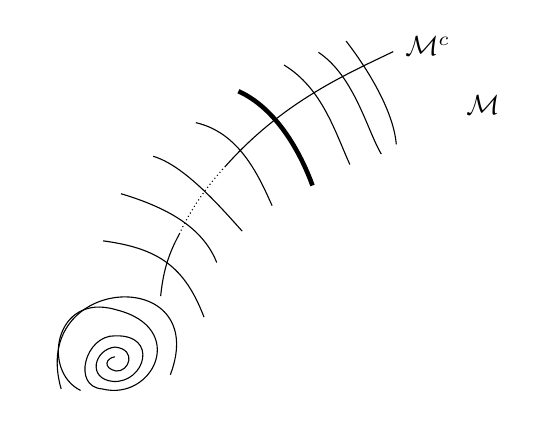
\begin{tikzpicture}[x=.95cm,y=.95cm]
\draw (1.49,1.36) .. controls (1.52,1.64) and (1.57,1.88) .. (1.74,2.19);
\draw[densely dotted] (1.74,2.19) .. controls (1.89,2.52) and (2.10,2.82) .. (2.35,3.09);
\draw (2.35,3.09) .. controls (3.12,3.96) and (3.98,4.33) .. (4.60,4.63);
\draw (.72,2.10) .. controls (1.46,2.00) and (1.81,1.76) .. (2.07,1.08);
\draw (.96,2.73) .. controls (1.56,2.55) and (2.05,2.29) .. (2.24,1.81);
\draw (1.39,3.23) .. controls (1.81,3.11) and (2.31,2.53) .. (2.58,2.23);
\draw (1.96,3.68) .. controls (2.53,3.55) and (2.79,3.00) .. (2.98,2.57);
\draw[line width=1.65pt] (2.53,4.10) .. controls (3.04,3.87) and (3.36,3.28) .. (3.52,2.84);
\draw (3.14,4.45) .. controls (3.65,4.14) and (3.82,3.56) .. (4.02,3.12);
\draw (3.60,4.62) .. controls (4.08,4.30) and (4.25,3.58) .. (4.44,3.26);
\draw (3.97,4.77) .. controls (4.31,4.33) and (4.61,3.79) .. (4.64,3.39);
\node[anchor=west] at (4.63,4.70) {\(\mathcal M^c\)};
\node at (5.80,3.92) {\(\mathcal M\)};
\draw (0.16,.12) .. controls (-.28,1.66) and (2.18,1.79) .. (1.62,.31);
\draw (0.42,.10) .. controls (-.11,.36) and (.08,1.42) .. (.89,1.18)
 .. controls (1.87,.94) and (1.39,-.05) .. (.71,.12)
 .. controls (.30,.15) and (.48,.84) .. (.88,.83)
 .. controls (1.47,.85) and (1.28,.20) .. (.86,.22)
 .. controls (.50,.25) and (.60,.65) .. (.88,.68)
 .. controls (1.18,.65) and (1.07,.34) .. (.89,.36)
 .. controls (.72,.40) and (.75,.53) .. (.88,.55);
\end{tikzpicture}}\endgroup}\par\smallskip
Нижний участок наклонной линии бледный. Слева у спирали соединение штрихов не установлено.}
\end{GelfandAdjacentEvidence}


Трюк Ф.-П.

\(\nu\) --- множитель (у интегр. по орбитам), к-рый будет выписан ниже.

На орбите есть 2 инв. метрики; а) огранич. метрики \(\mathcal M\): \(dg\)

б) [Своя естеств. метрика (перенесённая с группы --- индуц. мер. на \(G/H\), \(H\)---стац. подгр.)]

\(\nu\) --- отношение двух мер на каждой орбите.


\Needspace{7\baselineskip}
\begin{GelfandAdjacentEvidence}{GELFAND-P001215}{1}
\SourcePage{GELFAND-P001215}{unlabelled}
\(\delta g\) --- вариация метрики --- кас. вектор к пр-ву метрик.
\begin{equation*}
\begin{aligned}
|\delta g|^2
&=\int_{\mathcal E}(\delta g,\delta g)\,\text{ф. объёма}
=\int_{\mathcal E}(\delta g,\delta g)\omega\\
&=\int_{\mathcal E}(\delta g,\delta g)\sqrt g\,d\xi_1\,d\xi_2
\end{aligned}\tag{8}
\end{equation*}
\begin{equation*}
\mathcal Dg\text{ --- форма объёма [вставлено: на }\mathcal M\text{], соотв. }|\delta g|^2\tag{9}
\end{equation*}
([переправленный знак] форма объёма, постр. по метрике)
\Unclear{GELFAND-P001215}{volume-overwrite}{Перед словами «форма объёма» переправлен знак, возможно « или \(=\).}
\end{GelfandAdjacentEvidence}
\begin{GelfandAdjacentEvidence}{GELFAND-P001215}{2}


\(L\) --- алгебра Ли группы диффеоморфизмов, т.е. алгебра Ли вект. полей на \(\mathcal E\).

\(\varepsilon\in L\)
\begin{equation*}
|\varepsilon|^2=\int_{\mathcal E}(\varepsilon,\varepsilon)\,\text{ф. объёма}
=\int_{\mathcal E}(\varepsilon,\varepsilon)\sqrt g\,d\xi_1\,d\xi_2\tag{10}
\end{equation*}
\begin{equation*}
\delta_\varepsilon g\in S^2(T^*)\tag{11}
\end{equation*}
\textit{[Справа:]} (вариация метрики по напр. \(\varepsilon\)).

\textit{[Под записью:]} --- производная Ли.
\Unclear{GELFAND-P001215}{lie-derivative-cancelled}{Под \(\delta_\varepsilon g\) зачёркнуто, предположительно, «вект. поля».}
\end{GelfandAdjacentEvidence}
\begin{GelfandAdjacentEvidence}{GELFAND-P001215}{3}


определим оператор:
\begin{equation*}
L=\Gamma(T)\overset{D}{\longrightarrow}\Gamma(S^2(T^*)),
\qquad D(\varepsilon)=\delta_\varepsilon g\tag{12}
\end{equation*}
\textit{[Под \(\Gamma(T)\):]} (вект. поля). (\(g\) фиксировано).
\Unclear{GELFAND-P001215}{tensor-power-overwrite}{У переправленного показателя при \(S\) в правой части (12) видна форма \(2\). Первоначальный знак неразборчив.}
\end{GelfandAdjacentEvidence}
\begin{GelfandAdjacentEvidence}{GELFAND-P001215}{4}

\begin{equation*}
\begin{aligned}
\|\varepsilon\|^2
&=\int_{\mathcal E}(D\varepsilon,D\varepsilon)\,\text{ф. объёма}\\
&=\int_{\mathcal E}(D\varepsilon,D\varepsilon)\sqrt g\,d\xi_1\,d\xi_2
\end{aligned}\tag{13}
\end{equation*}
\begin{equation*}
\frac{\text{ф. объёма, отв. }\|\quad\|}{\text{ф. объёма, отв. }\lvert\quad\rvert}
=(\det\Delta)^{1/2},\qquad\text{где }\Delta=D^*D\tag{14}
\end{equation*}
\textit{[На правом поле, за двойной чертой:]} \(\Delta\) --- опер. Лапласа на вект. полях;
\(\Delta:\Gamma(T)\to\Gamma(T)\).

Отношение (14) и есть по определению множитель \(\nu\) в (7)
\[
\Gamma(S^2T)\subset\Gamma(\operatorname{Hom}(T,T))
\]
\textit{[Под \(\operatorname{Hom}(T,T)\), фигурная скобка:]} скаляры \(\oplus\) след 0.

\textit{[Справа:]} (из-за метрики); (отожд. \(S^2T\), \(S^2T^*\) и влож. в \(\operatorname{Hom}(T,T)\)).

Соотв. разложения сечений:
\begin{equation*}
\Gamma(S^2T)=\Gamma(S^2T)^c\oplus\Gamma(S^2T)^{\mathrm{diff}}\tag{15}
\end{equation*}
\textit{[Под первым слагаемым:]} конформные изменения метрики.

\textit{[Под вторым слагаемым:]} измен. под действ. производных Ли.

[зачёркнуто]
\begin{equation*}
(S^2T)^{\mathrm{diff}}=T\otimes\Omega^{0,1}\tag{16}
\end{equation*}
\Unclear{GELFAND-P001215}{eq16-cancelled}{Перед левой частью (16) зачёркнут знак, возможно \(\Gamma\) или \(\Phi\).}
\end{GelfandAdjacentEvidence}
\begin{GelfandAdjacentEvidence}{GELFAND-P001215}{5}

\Unclear{GELFAND-P001215}{bundle-splitting}{Надстрочное обозначение в (16) читается «diff». Смысл этого обозначения в равенстве не уточнён.}
\end{GelfandAdjacentEvidence}
\begin{GelfandAdjacentEvidence}{GELFAND-P001215}{6}


[зачёркнуто] Оказывается, что
\begin{equation*}
D=\bar\partial:\Gamma(T)\longrightarrow\Gamma(T\otimes\Omega^{0,1})\tag{17}
\end{equation*}
\Unclear{GELFAND-P001215}{before-eq17-cancelled}{Перед «Оказывается, что» зачёркнут неразборчивый знак.}
\end{GelfandAdjacentEvidence}


[Метрика опред. на \(\mathcal E\) комплексную структуру; поэтому имеет смысл \(\Omega^{0,1}\)]
\[
(S^2T)^{\mathrm{diff}}\sim\text{-матр. }\begin{pmatrix}a&b\\b&-a\end{pmatrix};
\]
смысл (16) --- матрица задаётся 1-й строкой.

\(T\) --- голом. расслоение, \(\Omega^{0,1}\) --- компл. 1-мерное расслоение.

\underline{на \(T\) действ.} гр. поворотов.

\(S^2T\) --- 3-мерное рассл., разложим под действием гр. поворотов.


\Needspace{7\baselineskip}
\begin{GelfandAdjacentEvidence}{GELFAND-P001216}{1}
\SourcePage{GELFAND-P001216}{80}
\uwave{Объяснение ф-лы} (14):

[\(\Delta\) --- оператор, отвеч. квадр. форме (13) относительно квадр. формы (10);].

Кстати:

\(\delta_\varepsilon g\) --- производная Ли метрики \(g\) по направлению \(\varepsilon\).

[2-й способ определить \(\Delta\) на \(\Gamma(T)\): отождествить \(T\) и \(T^*\)
с пом. метрики и взять \(\Delta\) на 1-формах.
Получ. то же самое, т.к. \(d\) (дифф. де Рама) и производная Ли двойственны друг другу].
\Unclear{GELFAND-P001216}{duality-statement}{Последняя строка скобки читается «и производная Ли двойственны друг другу». Спаривание в записи не указано.}
\end{GelfandAdjacentEvidence}


\(S^2T=S^2T^*\) в присутствии метрики.


\Needspace{7\baselineskip}
\begin{GelfandAdjacentEvidence}{GELFAND-P001217}{1}
\SourcePage{GELFAND-P001217}{unlabelled}
\underline{\underline{21/X--85.}}\qquad \uwave{Сем. Гельфанда.}

\underline{\underline{Рыжикова}} (ученица А. Семенова, 5-й курс).

\uwave{Алгоритм того, как проверить любое тождество в структуре подпр-в} [зачёркнуто] \uwave{конечномерного пр-ва}.
\Incomplete{GELFAND-P001217}{struck-prefix}{Зачёркнутая скобочная запись перед «конечномерного пр-ва» не прочитана.}
\end{GelfandAdjacentEvidence}
\begin{GelfandAdjacentEvidence}{GELFAND-P001217}{2}


Видим,, для какой размерности достаточно проверять [зачёркнуто]
\Unclear{GELFAND-P001217}{dimension-final-mark}{После «проверять» зачёркнут знак, возможно \(2\) или вопросительный знак.}
\end{GelfandAdjacentEvidence}
\begin{GelfandAdjacentEvidence}{GELFAND-P001217}{3}

\[
a(ab+c)=ab+ac\qquad\text{или}\qquad
a(b+c)=ab+ac\quad\text{при }b\leq a
\]
\textit{[Ниже:]} дост. в 2-мерном.

Общая формула: достат. проверять в пр-ве размерности
\[
n=\min[\max(d(p),d(q)),\max(k(p),k(q))]+1
\]
\(p,q\) --- 2 зад. терма

\(d(p)\) --- число сложений в \(p\) (дизъюнкция)

\(k(p)\) --- ″ --- умножений в \(p\) (конъюнкция)

В пр-ве фикс. разм. (над \(\mathbb R\)) есть алг. Тарского.

\Needspace{6\baselineskip}
\underline{\underline{Фукс}} (по Фейгину). \underline{Продолжение} \uwave{о струнах}.

Надо вычислить интеграл:
\begin{equation*}
\int_{\mathcal M^c}(\operatorname{Det}\Delta)^{-d/2}\nu\tag{1}
\end{equation*}
\underline{Фейгин.}

Надо сосчитать интеграл
\begin{equation*}
\int_{\mathcal M_t}(\operatorname{Det}\Delta_0)^{-d/2}\mathcal Dg
=\int_{\mathcal M_t^c}\frac{\operatorname{Det}\Delta_1}{(\operatorname{Det}\Delta_0)^{d/2}}\mathcal Dg,\tag{2}
\end{equation*}
\Unclear{GELFAND-P001217}{eq2-domain-cancelled}{В (2) у \(\mathcal M_t\) под первым интегралом зачёркнут верхний знак, возможно \(c\).}
\end{GelfandAdjacentEvidence}
\begin{GelfandAdjacentEvidence}{GELFAND-P001217}{4}

\Unclear{GELFAND-P001217}{eq2-cancelled-formula}{Запись справа от (2) зачёркнута; возможно \(\Delta=\Delta_0\) или \(\Delta\ne\Delta_0\).}
\end{GelfandAdjacentEvidence}
\begin{GelfandAdjacentEvidence}{GELFAND-P001217}{5}

\EvidenceBlock{GELFAND-P001217}{eq2-determinant-power}{В числителе написано \(\operatorname{Det}\Delta_1\) без показателя степени. У знаменателя стоит степень \(d/2\).}{}
\end{GelfandAdjacentEvidence}


\(\mathcal M\) --- пр-во метрик, \(t\) --- точка пр-ва модулей кривых рода \(g\)

\(\mathcal M_t\) --- пр-во метрик, отвеч. компл. структуре, соотв. модулю \(t\).


\Needspace{7\baselineskip}
\begin{GelfandAdjacentEvidence}{GELFAND-P001218}{1}
\SourcePage{GELFAND-P001218}{87}
\(\mathcal M_t^c\) --- мн-во метрик [вставлено над строкой: (соотв. зад. модулю \(t\))] вида \(e^\varphi g_0\),
где \(g_0\) --- метрика пост. отриц. кривизны \(=-1\).
\Unclear{GELFAND-P001218}{upper-margin-abbreviation}{В приписке под \(\mathcal M_t^c\) читается «на пв., соотв. \(t\)». Сокращение «пв.» может означать «пов.».}
\end{GelfandAdjacentEvidence}
\begin{GelfandAdjacentEvidence}{GELFAND-P001218}{2}


\(T\) --- касательное расслоение на кривой (уже с компл. структурой)
\[
\bar\partial:\Gamma(T^j)\longrightarrow\Gamma(T^j\otimes\Omega^{0,1}),
\qquad\Delta_j=\bar\partial^*\bar\partial
\]
\Unclear{GELFAND-P001218}{gamma-cancelled-parenthesis}{После \(T^j\), перед \(\otimes\), видна верхняя дуга зачёркнутого знака, предположительно закрывающей скобки.}
\end{GelfandAdjacentEvidence}
\begin{GelfandAdjacentEvidence}{GELFAND-P001218}{3}


На самом деле \(\mathcal M_t^c\) [зачёркнуто]; \(\mathcal M_t^c\subset\mathcal M_t\)
[зачёркнуто]
\Unclear{GELFAND-P001218}{mt-cancelled-mark}{После первого \(\mathcal M_t^c\) зачёркнут неразобранный знак.}
\end{GelfandAdjacentEvidence}
\begin{GelfandAdjacentEvidence}{GELFAND-P001218}{4}

\Unclear{GELFAND-P001218}{mt-cancelled-inclusion}{Справа зачёркнуто, предположительно \((\mathcal M^c\subset\mathcal M_t)\) или \((\mathcal M_t^c\subset\mathcal M_t)\).}
\end{GelfandAdjacentEvidence}
\begin{GelfandAdjacentEvidence}{GELFAND-P001218}{5}


(\(t\) фиксировано).

Всякая метрика из \(\mathcal M_t\) может быть (действием \(\operatorname{Diff}\))
\EvidenceBlock{GELFAND-P001218}{unfinished-sentence}{Фраза обрывается после «(действием Diff)».}{}
\end{GelfandAdjacentEvidence}
\begin{GelfandAdjacentEvidence}{GELFAND-P001218}{6}


Пр-во модулей имеет размерность \(\underline{3g-3}\).

Интеграл по нему ещё не вычислен (этим много занимаются).

\Incomplete{GELFAND-P001218}{mid-cancelled-formula}{Короткая зачёркнутая формула перед строкой о \(\operatorname{Det}\Delta_0\) не прочитана.}
\end{GelfandAdjacentEvidence}
\begin{GelfandAdjacentEvidence}{GELFAND-P001218}{7}


\(\operatorname{Det}\Delta_0\) --- берётся по ненулевым собственным значениям.

\(\operatorname{Det}\Delta_j=\operatorname{Det}\Delta_j(\varphi)\).

Далее,
\begin{equation*}
\begin{aligned}
\delta\ln\operatorname{Det}\Delta_j(\varphi)
&=(Aj+B)\int_{\mathcal E}\delta\varphi\cdot\operatorname{Vol}\\
&\quad+C(6j^2+6j+1)\int_{\mathcal E}\delta\varphi\cdot K\cdot\operatorname{Vol}
\end{aligned}\tag{3}
\end{equation*}
\Unclear{GELFAND-P001218}{eq3-coefficient}{Первоначальный коэффициент зачёркнут. Вставка читается как \((Aj+B)\), возможно \((A_j+B)\).}
\end{GelfandAdjacentEvidence}
\begin{GelfandAdjacentEvidence}{GELFAND-P001218}{8}

\EvidenceBlock{GELFAND-P001218}{eq3-denominator-cancelled}{Под левой частью зачёркнуты дробная черта и знаменатель \(\delta\varphi\).}{}
\end{GelfandAdjacentEvidence}
\begin{GelfandAdjacentEvidence}{GELFAND-P001218}{9}


\textit{[Под первым \(\operatorname{Vol}\), фигурная скобка:]} форма объёма.

(\(j\) --- «спин»)

\(A,B,C\) --- нек-рые постоянные; \(K\) --- гауссова кривизна поверхности.
\[
\begin{aligned}
j=1&\Rightarrow 6j^2+6j+1=13\\
j=0&\Rightarrow 6j^2+6j+1=1
\end{aligned}
\]
\Unclear{GELFAND-P001218}{j-zero-value-overwritten}{У переправленного результата в строке \(j=0\) видна форма \(1\). Первоначальная запись неразборчива.}
\end{GelfandAdjacentEvidence}
\begin{GelfandAdjacentEvidence}{GELFAND-P001218}{10}


При \(d=26\) происходит сокращение аномалии.

И тогда интегрировать нужно константу (в прав. части (2))

\underline{Следствие}:
\begin{equation*}
\ln\operatorname{Det}\Delta_j(\varphi)
=A\int\text{[зачёркнуто]}\,\varphi\cdot\partial\bar\partial\varphi
+B\int e^\varphi\operatorname{Vol}
+C\int\varphi\operatorname{Vol}+D\tag{4}
\end{equation*}
\Unclear{GELFAND-P001218}{eq4-cancelled-term}{Сразу после первого знака интеграла в (4) зачёркнуто выражение, возможно \(\partial\varphi\wedge\bar\partial\varphi\) или \(\partial\varphi\,\bar\partial\varphi\).}
\end{GelfandAdjacentEvidence}


(\(A,B,C,D\) --- постоянные)

\(\Rightarrow\) вычисление эквив. ур-ю Лиувилля (в (4) его лагранжиан)

Реш. ур-я Лиув. эквивалентно вычислению
\begin{equation*}
\int e^{\mathcal L_j(\varphi)}\mathcal D\varphi,\tag{5}
\end{equation*}
где \(\mathcal L_j(\varphi)\) --- левая (\(=\) правая) часть (4)

\(\ln\operatorname{Det}\Delta_j\) берётся как лагранжиан новой теории. Ясно, что
\begin{equation*}
(2)=\int e^{\mathcal L_1(\varphi)-\frac d2\mathcal L_0(\varphi)}\mathcal D\varphi.\tag{6}
\end{equation*}


\clearpage
\pdfbookmark[0]{Глава 27}{gelfand-archive-chapter-27}
\section*{Глава 27}
\Needspace{7\baselineskip}
\begin{GelfandAdjacentEvidence}{GELFAND-P001219}{1}
\SourcePage{GELFAND-P001219}{unlabelled}
\underline{\(28/\overline{\underline{X}}\)---85 г.}\qquad \underline{Сем. Гельфанда}

\underline{W. Müller.}

\uwave{Cheeger / Gromov}

\(X\) --- полное рим. мн-гие, \(\operatorname{vol}(X)<\infty\), \(\lvert K\rvert<1\).

\textit{[Под \(K\):]} секц. кривизна.
\[
\int p(\Omega)\;-\;?
\]
\underline{Теор.} \(X\) --- внутренность комп. мн-гия с краем
\textit{[Под словом «внутренность»: (диффеоморфно)]}
\[
\Rightarrow 1)\;\int_X p(\Omega)=\chi(X).
\]
\Unclear{GELFAND-P001219}{formula-cancellation}{Над \(p(\Omega)\) зачёркнут неразобранный знак.}
\end{GelfandAdjacentEvidence}



\Needspace{7\baselineskip}
\begin{GelfandAdjacentEvidence}{GELFAND-P001220}{1}
\SourcePage{GELFAND-P001220}{unlabelled}
\begin{equation*}
2)\quad \int_X L_k(p_1,\ldots,p_k)\quad\text{--- гомотопич. инвариант}
\end{equation*}
Вопрос, связ. с раб. \underline{Cheeger'а}

mfd [вставлено над строкой \(X\)] with cone like singularity

\SourceFigure{GELFAND-P001220}{cone-sketch}{%
\par\smallskip
{\color{black}\begingroup\color{black}\GelfandFitDiagram{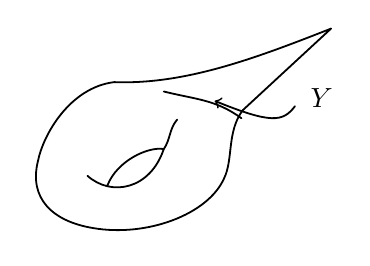
\begin{tikzpicture}[x=.17mm,y=.17mm,line width=.65pt,line cap=round,line join=round]
\draw (269,153) .. controls (213,131) and (160,111) .. (107,113)
 .. controls (74,109) and (54,74) .. (50,54)
 .. controls (43,26) and (61,9) .. (91,4)
 .. controls (131,-3) and (177,14) .. (189,41)
 .. controls (196,55) and (191,76) .. (203,92) -- cycle;
\draw (87,43) .. controls (105,27) and (134,33) .. (144,63)
 .. controls (132,65) and (109,54) .. (102,36);
\draw (144,63) .. controls (149,70) and (148,78) .. (154,85);
\draw (144,106) .. controls (168,100) and (183,100) .. (202,86);
\draw[->] (242,95) .. controls (233,83) and (224,82) .. (182,99);
\node at (262,101) {\(Y\)};
\end{tikzpicture}}\endgroup}\par\smallskip
Штрихи указателя у сужения накладываются друг на друга.}
\end{GelfandAdjacentEvidence}
\begin{GelfandAdjacentEvidence}{GELFAND-P001220}{2}


\(\Delta\) on \(\Lambda^*\)

\(\Delta\) on cone
\begin{equation*}
-\frac{\partial^2}{\partial u^2}+u^{-2}A(u)
\end{equation*}
\begin{equation*}
A(u)\in L^2((0,1],\Lambda^*(Y))
\end{equation*}
\Unclear{GELFAND-P001220}{function-or-operator}{В обеих строках написано \(A(u)\). В первой строке стоит знак принадлежности, во второй записано отображение. Во второй строке \(u\) наведено повторно. Роль \(A(u)\) в этих двух строках неясна.}
\end{GelfandAdjacentEvidence}
\begin{GelfandAdjacentEvidence}{GELFAND-P001220}{3}

\begin{equation*}
\begin{gathered}
A(u):\Lambda^*(Y)\longrightarrow\Lambda^*(Y),\\
C(Y)=(0,1]\times Y,\\
ds^2=du^2+u^{-2}g_Y.
\end{gathered}
\end{equation*}
\EvidenceBlock{GELFAND-P001220}{cone-metric-exponent}{В показателе степени у \(u\) перед \(g_Y\) написано \(-2\).}{Запись в рукописи.}
\end{GelfandAdjacentEvidence}

\begin{equation*}
\operatorname{Tr}(e^{-t\Delta})\underset{t\to0+}{\sim}
\sum_{j\geq0}a_jt^{-(n-j)/2}+c\log t+b
\end{equation*}
\begin{equation*}
b=b_0\zeta_Y(-1)+\sum_{j\geq1}b_j
\underset{s=2j-1}{\operatorname{Res}}\zeta_Y(s)
\end{equation*}
\begin{equation*}
\zeta_Y(s)=\sum_{\lambda_j}\lambda_j^{-s}
\end{equation*}
\begin{equation*}
D_s=d+\delta:\Lambda^*_+(X)\longrightarrow\Lambda^*_-(X)
\qquad\text{signature operator}
\end{equation*}
опер. сигнатуры
\begin{equation*}
(*)\qquad \operatorname{Ind}D_s=\int_X L_k(p_1,\ldots,p_k)+\eta_Y(B),
\qquad\text{где \(B\) опр. ниже.}
\end{equation*}
\(\dim X=4k\).

[Под скобкой у интеграла] такой был бы индекс без края.

[Выделено скобкой] \(L_k=0\) \uwave{на конусе}.

На конусе:
\begin{equation*}
d+\delta=D_s=-\frac{\partial}{\partial u}+u^{-1}B,
\qquad B:\Lambda^*(Y)\longrightarrow\Lambda^*(Y).
\end{equation*}
[Справа, за двойной вертикальной чертой] На \(\Lambda^{ev}\) \(B\) имеет вид \(\pm(*d-d*)\).
\begin{GelfandAdjacentEvidence}{GELFAND-P001220}{4}
\begin{equation*}
D=\frac{\partial^n}{\partial u^n}+\sum u^{i-n}\frac{\partial^i}{\partial u^i}A_j
\end{equation*}
\EvidenceBlock{GELFAND-P001220}{operator-indices}{В показателе при \(u\) и в обоих показателях при знаке производной написано \(i\). У \(A_j\) стоит индекс \(j\). Пределы суммы не выписаны.}{Запись в рукописи.}
\end{GelfandAdjacentEvidence}


\(A_j\) --- дифф. оп. на \(Y\).

\uwave{индекс --- ?}

В примере Чигера возникает \(\eta\)! --- ф-ла \((*)\)


\Needspace{7\baselineskip}
\begin{GelfandAdjacentEvidence}{GELFAND-P001221}{1}
\SourcePage{GELFAND-P001221}{6}
Индекс определяется на ф-ях, удовл. [зачёркнуто] условию на особенности:
\Unclear{GELFAND-P001221}{top-cancellation}{Зачёркнутое слово перед «условию» не разобрано.}
\end{GelfandAdjacentEvidence}
\begin{GelfandAdjacentEvidence}{GELFAND-P001221}{2}

\begin{equation*}
\lim_{u\to0}u^{-1/2}\varphi(u)=\lim_{u\to0}u^{1/2}\varphi'(u)
\end{equation*}
\uwave{Связь с представлениями.}
\begin{equation*}
X=K\backslash G/\Gamma\qquad\text{loc symm.},\quad\operatorname{vol}(X)<\infty
\end{equation*}
\(\mathcal E,\mathcal F\longrightarrow X\)\quad loc. [зачёркнуто]
[над строкой: triv.\ (?)] vectorbundles
\Unclear{GELFAND-P001221}{bundle-correction}{Над зачёркнутым написано «triv. (?)». Начальный штрих зачёркнутого сокращения допускает чтение «triv.», остальные буквы закрыты зачёркиванием.}
\end{GelfandAdjacentEvidence}
\begin{GelfandAdjacentEvidence}{GELFAND-P001221}{3}

\begin{equation*}
D:C_0^\infty(X,\mathcal E)\longrightarrow C_0^\infty(X,\mathcal F)
\qquad\text{oper. loc inv.}
\end{equation*}
\underline{Th.}
\begin{equation*}
\begin{gathered}
\ker\bar D<\infty,\\
\ker\bar D^*<\infty.
\end{gathered}
\end{equation*}
\begin{equation*}
\operatorname{Ind}_{L^2}D=\dim\ker\bar D-\dim\ker\bar D^*
\end{equation*}
\begin{center}\rule{.9em}{.35pt}\quad\rule{.9em}{.35pt}\end{center}
\begin{equation*}
X=H\times H/SL(2,O_F),\qquad F=Q(\sqrt D),\quad D>0.
\end{equation*}
\Unclear{GELFAND-P001221}{group-cancellation}{Перед \(O_F\) в \(SL(2,O_F)\) густо зачёркнутый знак.}
\end{GelfandAdjacentEvidence}
\begin{GelfandAdjacentEvidence}{GELFAND-P001221}{4}


only 1 cusp
\begin{equation*}
D_s=d+\delta:\Lambda^*_+(X)\longrightarrow\Lambda^*_-(X)
\end{equation*}
\begin{equation*}
\operatorname{ind}D_s=\frac13\int_X p_1-\frac1{2\pi}L(M,V,1)\operatorname{vol}(\mathbb R^2/M)
\end{equation*}
\Unclear{GELFAND-P001221}{integrand-mark}{После \(p_1\) перед знаком минуса густо затушёванный знак, похожий на \(A\) или \(\Delta\). Неясно, зачёркнут ли он.}
\end{GelfandAdjacentEvidence}
\begin{GelfandAdjacentEvidence}{GELFAND-P001221}{5}

\begin{equation*}
M=O_F,\qquad V=O_F^{*2}
\end{equation*}
\begin{equation*}
L(M,V,s)=\sum_{\mu\in(M-0)N_F}\frac{\operatorname{sign}N(\mu)}{|N(\mu)|^s}
\end{equation*}
\EvidenceBlock{GELFAND-P001221}{sum-domain}{Под суммой после закрывающей круглой скобки непосредственно написано \(N_F\).}{Запись в рукописи.}
\end{GelfandAdjacentEvidence}
\begin{GelfandAdjacentEvidence}{GELFAND-P001221}{6}


\underline{\underline{Фейгин.}}\qquad\uwave{О струнах}\qquad(раб. \underline{Полякова})

(\underline{Продолжение.})

\(\mathcal E\) --- рим. поверхность рода \(g\)

\(T\) --- кас. рассл.

На \(\mathcal E\) выбрана компл. структура, индуц. рим. метрикой, и оператор \(\bar\partial:T^j\longrightarrow T^j\otimes\Omega^{0,1}\);
\begin{equation*}
\Delta_j=\bar\partial^*\bar\partial
\end{equation*}
\begin{equation*}
0\longrightarrow H^0(T^j)\longrightarrow\Gamma(T^j)
\overset{\bar\partial}{\longrightarrow}\Gamma(T^j\otimes\Omega^{0,1})
\longrightarrow H^1(T)\longrightarrow0.\tag{1}
\end{equation*}
\EvidenceBlock{GELFAND-P001221}{sequence-final-term}{Перед нулём в (1) написано \(H^1(T)\). У \(T\) нет показателя.}{Запись в рукописи.}
\end{GelfandAdjacentEvidence}



\Needspace{7\baselineskip}
\begin{GelfandAdjacentEvidence}{GELFAND-P001222}{1}
\SourcePage{GELFAND-P001222}{unlabelled}
Задачу можно переформулир. как вычисление кручения Рэя --- Зингера этого комплекса.
\begin{equation*}
g_{ij}\longrightarrow g_{ij}(1+\varepsilon\rho)\tag{2}
\end{equation*}
\(\bar\partial\) имеет \(\ker\) и \(\operatorname{coker}\).
[В той же межстрочной записи:] На самом деле вычислялось изменение

кручения Рэя --- Зингера [зачёркнуто] комплекса (1) при деформации
\Unclear{GELFAND-P001222}{torsion-cancellation}{Справа в зачёркнутой записи после «Зингера» виден знак, похожий на \(\bar\partial\). В середине, возможно, написано \(\operatorname{Det}\).}
\end{GelfandAdjacentEvidence}
\begin{GelfandAdjacentEvidence}{GELFAND-P001222}{2}


на \(\Gamma(T^j)\) и на \(\Gamma(T^j\otimes\Omega^{0,1})\)
имеются эрмитовы метрики.

Они индуцируют эрм. метрики на \(\underbrace{H^0(T^j)}_{\text{подпр-во}}\) и \(H^1(T^j)\).

\(\ker\bar\partial\bar\partial^*\) отожд. с \(H^1(T^j)\)
\(\Rightarrow\) на \(H^1(T^j)\) имеется эрм. метрика.
\begin{equation*}
\operatorname{Det}T^j:=\Lambda^{\max}H^0(T^j)
\otimes\bigl(\Lambda^{\max}H^1(T^j)\bigr)^*\tag{3}
\end{equation*}
(термин. Quillen'а)\qquad(1-мерное пр-во)

(4) На \(\operatorname{Det}T^j\) тоже есть эрмитова метрика. Обозначим её \(\varepsilon\).

Кручение Рэя --- Зингера --- другая эрм. метрика на \(\operatorname{Det}T^j\). Она равна эрм. метрике (4), делённой на \(\operatorname{Det}\Delta_j\):
\begin{equation*}
\frac{\varepsilon}{\operatorname{Det}\Delta_j}\tag{5}
\end{equation*}
Рассм. вариацию метрики:
\begin{equation*}
g_{ij}\longrightarrow g_{ij}(1+\varepsilon\rho)\tag{6}
\end{equation*}
Пусть даны послед. чисел \(j_1,j_2,\ldots,j_n\),
[вставлено над строкой: \(k_1,\ldots,k_n\)] и 1-мерное пр-во
\begin{equation*}
\operatorname{Det}(T^{j_1})^{k_1}\otimes
\operatorname{Det}(T^{j_2})^{k_2}\otimes\cdots\otimes
\operatorname{Det}(T^{j_n})^{k_n}\tag{7}
\end{equation*}
с эрм. метрикой \(=\) произведению кручений Рэя --- Зингера каждого из этих пр-в.

(8) \underline{Утв.} Метрика на (7) не мен. при вариации (6), если
\begin{equation*}
\sum_\alpha(6j_\alpha^2+6j_\alpha+1)k_\alpha=0.\tag{9}
\end{equation*}
\Unclear{GELFAND-P001222}{anomaly-extra-stroke}{Между \(\sum_\alpha\) и открывающей скобкой виден отдельный густой наклонный штрих. Первая цифра \(6\) обведена. Назначение отдельного штриха неясно.}
\end{GelfandAdjacentEvidence}
\begin{GelfandAdjacentEvidence}{GELFAND-P001222}{3}


\uwave{Или:} при этом условии (9) метрика на (7) зависит только от компл. структуры.

Пусть \(\mathcal M\) --- мн-гие модулей комплексных кривых рода \(g\).

Набор пр-в --- 1-мерное расслоение на \(\mathcal M\).

Постр. метрика на этом расслоении (похожая констр. есть у [Фальтингса?])
\Unclear{GELFAND-P001222}{final-name}{Фамилия в конце строки предположительно читается «Фальтингса». Из-за соединения последних штрихов возможно чтение «Фальтинга».}
\end{GelfandAdjacentEvidence}



\Needspace{7\baselineskip}
\begin{GelfandAdjacentEvidence}{GELFAND-P001223}{1}
\SourcePage{GELFAND-P001223}{unlabelled}
\(4/\overline{\underline{\mathrm{XI}}}-85\)\quad\underline{Сем. Гельфанда}

\underline{\underline{Рыжикова}}\quad\underline{О представлениях структур.}
(раб. Гельфанда и Пономарёва)

\underline{Опр.} Элем. \(a\in L\) наз. \uwave{совершенным}, если

(\(L\) --- структура)
\begin{equation*}
\begin{gathered}
\forall k,\quad\forall\rho:L\longrightarrow\mathcal L(V),\quad\exists U\subseteq V,\\
U+\rho(a)=V,\qquad U\rho(a)=0,\\
\forall x:\quad\rho(x)=\rho(a)\rho(x)+U\rho(x).
\end{gathered}
\end{equation*}
[Над \(k\) --- поле. Над \(\rho\) --- предст..]

Или: \(\forall\) неразложимого предст. \(a\) отобр. в \(0\) или во всё пр-во.
\Unclear{GELFAND-P001223}{perfect-element-overwrite}{Поверх переправленного знака перед «отобр.» читается строчное \(a\). Первоначальные штрихи неразличимы.}
\end{GelfandAdjacentEvidence}
\begin{GelfandAdjacentEvidence}{GELFAND-P001223}{2}


\underline{Опр. структуры.}

\(a+b\), \(a\cdot b\) --- асс. коммут.
\begin{equation*}
\begin{gathered}
a\cdot a=a,\qquad a+a=a,\qquad a(a+b)=a,\qquad a+ab=a,\\
a\leq b\Longleftrightarrow ab=a\Longleftrightarrow a+b=b,\\
a\leq b\Longrightarrow b(a+c)=a+bc.
\end{gathered}
\end{equation*}
Предст. структуры \(\rho:L\longrightarrow\mathcal L(V)\).

\begin{center}\rule{.9em}{.35pt}\quad\rule{.9em}{.35pt}\end{center}

[Зачёркнуто: Рассмотрим.] [Над строкой: Построим.] счётное число кубиков \(B^+(\ell)\) и \(B^-(\ell)\),
\(\ell\geq1\),
\EvidenceBlock{GELFAND-P001223}{construct-verb-correction}{Над зачёркнутым «Рассмотрим» вписано «Построим».}{Запись в рукописи.}
\end{GelfandAdjacentEvidence}


\(D^r\) --- своб. модулярная решётка с \(r\) образ. \(e_1,\ldots,e_r\).


\Needspace{7\baselineskip}
\begin{GelfandAdjacentEvidence}{GELFAND-P001224}{1}
\SourcePage{GELFAND-P001224}{unlabelled}
1.\ \underline{\(\ell=1\)}

Положим \(h_t(1)=\displaystyle\sum_{j\ne t}e_j\), \(t=1,\ldots,r\).

Эти \(h_t(1)\) [вставлено над зачёркнутым: порождают] булевскую алгебру
\(B^+(1)\) [зачёркнуто]
\Unclear{GELFAND-P001224}{upper-cancellation}{Зачёркнутая запись после \(B^+(1)\) предположительно начинается словом «уже». Остальная запись неразборчива.}
\end{GelfandAdjacentEvidence}
\begin{GelfandAdjacentEvidence}{GELFAND-P001224}{2}

\begin{equation*}
\begin{gathered}
0,\ h_1,\ldots,h_4,\quad h_1\cdot h_2,\ h_2\cdot h_3,\\
h_1\cdot h_2\cdot h_3,\ldots,\\
h_1\cdot h_2\cdot h_3\cdot h_4.
\end{gathered}
\end{equation*}
Сумма произв. уже выраж. через произведение.

2.\ \uwave{\(\ell=2\)}
\begin{equation*}
\{(i_1,i_2):i_1\ne i_2\}=A(r,2)
\end{equation*}
\begin{equation*}
\{(i_1,t),\ i_1\ne t\}=A_t(r,2)\qquad(t\text{ --- фиксировано})
\end{equation*}
\begin{equation*}
e_t(2)=\sum_{i_1=1}^{r}e_{i_1t}
=\sum e_{i_1}\left(\sum_{k\ne i_2,t}e_k\right)
\end{equation*}
\EvidenceBlock{GELFAND-P001224}{second-level-sum}{Пределы первой суммы написаны \(i_1=1\) и \(r\). Под внутренней суммой написано \(k\ne i_2,t\).}{Запись в рукописи.}
\end{GelfandAdjacentEvidence}
\begin{GelfandAdjacentEvidence}{GELFAND-P001224}{3}

\begin{equation*}
h_t(2)=\sum_{j\ne t}e_j(2)
\end{equation*}
\begin{center}\rule{.9em}{.35pt}\quad\rule{.9em}{.35pt}\end{center}
\begin{equation*}
\{(i_1,\ldots,i_\ell),\ i_j\ne i_{j+1}\}=A(r,\ell)
\end{equation*}
\begin{equation*}
\{(i_1,\ldots,i_{\ell-1},t),\ i_{\ell-1}\ne t\}\cap A(r,\ell)=A_t(r,\ell)
\end{equation*}
\begin{equation*}
\Gamma(i_1,\ldots,i_\ell)=\{\beta=(k_1,\ldots,k_{\ell-1})\mid k_j\notin\{j_{i-1},j_i\}
\end{equation*}
\Unclear{GELFAND-P001224}{gamma-index}{Начальный знак предположительно читается как \(\Gamma\), возможно \(\Pi\). Последние два знака с нижними индексами похожи на \(j\). Индексы предположительно читаются как \(i-1\) и \(i\). Справа видна одна закрывающая фигурная скобка.}
\end{GelfandAdjacentEvidence}
\begin{GelfandAdjacentEvidence}{GELFAND-P001224}{4}


Все это кубики (сост. из \(2^n\) элем.) --- булевы алгебры;
нижние строятся двойств. образом.
\EvidenceBlock{GELFAND-P001224}{cardinality-exponent}{В показателе степени при \(2\) написано \(n\).}{Запись в рукописи.}
\end{GelfandAdjacentEvidence}
\begin{GelfandAdjacentEvidence}{GELFAND-P001224}{5}


Все они упорядочены.

\underline{Опр.} \(V\) над \(K\) [затушёвано] хар-ки \(0\)
\Unclear{GELFAND-P001224}{char-cancellation}{Между \(K\) и «хар-ки» густо затушёванный знак.}
\end{GelfandAdjacentEvidence}


\(\rho:L\longrightarrow\mathcal L(V,K)\) наз. вполне неприводимым, если
\begin{equation*}
\rho(L)\cong\mathcal L(\mathbb Q^n)\cong P(n-1,\mathbb Q).
\end{equation*}


\Needspace{7\baselineskip}
\begin{GelfandAdjacentEvidence}{GELFAND-P001225}{1}
\SourcePage{GELFAND-P001225}{10}
\underline{\underline{Б.Л. Фейгин}}\qquad\underline{О струнах}

\underline{Как появляется алг. Вирасоро и гипергеометрич. ф-и?}

\uwave{Алгебра Вирасоро}: алг. Ли \(\mathcal L\) с базисом
\(\{e_i\}\), \(\underline{\underline{C}}\), \(i\in Z\).
\begin{equation*}
\begin{gathered}
\relax [e_i,e_j]=(j-i)e_{i+j}+\delta_{i,-j}\frac{i^3-i}{12}\underline{\underline{C}},\\[0pt]
[e_i,\underline{\underline{C}}]=0.
\end{gathered}\tag{1}
\end{equation*}
(2) Фактор по центру \(=\) алг. вект. полей на окружности.

Модули Верма см. в книге \uwave{Диксмье} об обёрт. алгебрах.

и 2 работы Бернштейна, [зачёркнуто] И.М.Г. и С.И. Гельфанда в ФА
\Unclear{GELFAND-P001225}{author-initials}{Перед «И.М.Г.» зачёркнута буква, предположительно «И». Возможно чтение «Н».}
\end{GelfandAdjacentEvidence}
\begin{GelfandAdjacentEvidence}{GELFAND-P001225}{2}


(в т.ч. о категориях Оре)
\Unclear{GELFAND-P001225}{category-reading}{После «категориях» читается «Оре». Значение слова неясно.}
\end{GelfandAdjacentEvidence}
\begin{GelfandAdjacentEvidence}{GELFAND-P001225}{3}

\begin{equation*}
\begin{gathered}
\mathfrak h=\{e_0,\underline{\underline{C}}\}\qquad(\text{картановская}),\\
\mathcal L_+=\{e_1,e_2,e_3,\ldots\}\qquad(\text{рожд.}),\\
\mathcal L_-=\{e_{-1},e_{-2},\ldots\}\qquad(\text{уничт.}).
\end{gathered}
\end{equation*}
\(\chi=(h,\bar{\bar{c}})\) --- [зачёркнуто] пара чисел
\Unclear{GELFAND-P001225}{pair-cancellation}{Зачёркнутое сокращение перед «пара» предположительно читается «упор.». Раскрытие сокращения неясно.}
\end{GelfandAdjacentEvidence}


Модуль Верма: \(M_\chi\), есть вак. вектор \(v\)
\begin{equation*}
\begin{cases}
e_0v=hv,\\
Cv=\bar{\bar{c}}\,v
\end{cases}
\qquad\mathcal L_-v=0.\tag{3}
\end{equation*}
Физики пишут \(L_i\) вместо \(e_i\).

(4) Дан \(M_\chi=M_{h,c}\), \uwave{когда} [вставлено над строкой: он]
\uwave{приводим}?

\begin{GelfandAdjacentEvidence}{GELFAND-P001225}{4}
Физики наз. это \uwave{массовыми ф-лами} (спектр масс)
\begin{equation*}
\begin{aligned}
0=\Phi_{k_1k_2}(h,c)
&=\prod_{j=1,2}\left\{h+\frac{c-13}{24}(k_j^2-1)+\frac12(k_1k_2-1)\right\}+\\
&\quad+\frac12(k_1^2-k_2^2)^2.
\end{aligned}\tag{5}
\end{equation*}
\EvidenceBlock{GELFAND-P001225}{kac-coefficient}{Коэффициент при \((k_1^2-k_2^2)^2\) в (5) написан \(1/2\). Знак плюс стоит и в конце предыдущей строки, и перед дробью.}{Запись в рукописи.}
\end{GelfandAdjacentEvidence}


(ф-ла Каца)

Здесь \(k_1,k_2\) --- натур. числа.

(6) \underline{Утв.} [Под заголовком: (Фейгин, Фукс).]
Если \(\exists\) \(k_1,k_2\), для к-рых выполнено (5), то предст. приводимо; если не сущ., то неприводимо.

(7) \underline{Добавление}: если \(M_\chi\) приводим, то в нём
\(\exists\) вектор, отличный от вак. и аннулируемый всеми опер. уничт. («особый вектор»).

\(\mathcal L\) естеств. градуирована \(\Rightarrow M_\chi\) тоже.


\Needspace{7\baselineskip}
\begin{GelfandAdjacentEvidence}{GELFAND-P001226}{1}
\SourcePage{GELFAND-P001226}{unlabelled}
(8) При этом уровень особ. вектора \(=k_1\cdot k_2\).

\uwave{Док-ва:} конструкции разных красивых предст. \uwave{2-х типов}.
\Unclear{GELFAND-P001226}{type-count}{Последняя запись цифры перед «-х типов» читается как \(2\). Первоначальные штрихи неразличимы.}
\end{GelfandAdjacentEvidence}
\begin{GelfandAdjacentEvidence}{GELFAND-P001226}{2}


\uwave{1-й тип.}
\begin{equation*}
\mathcal L/C\longrightarrow gl_\infty,\ O_\infty,\ sp_\infty
\end{equation*}
[Под фактором: (в. поля).]
\Unclear{GELFAND-P001226}{quotient-centre}{Переправленный знак после косой черты предположительно читается как \(C\). Регистр буквы неясен, возможно \(c\).}
\end{GelfandAdjacentEvidence}
\begin{GelfandAdjacentEvidence}{GELFAND-P001226}{3}


\uwave{2-й тип}

(9) \(\mathcal L\hookrightarrow\) обёртыв. алгебру аффинной алгебры Каца--Муди.

Строим вложение

\(\mathfrak g\) --- конечномерн. простая алг. Ли

\(\widehat{\mathfrak g}\) --- одномерное расшир. алгебры токов (обычно назыв. алг. Каца--Муди)

[Между строками:] ([зачёркнуто] \uwave{И.М.Г.} Алг. токов --- алг. матр. ф-й на окружности).
\Unclear{GELFAND-P001226}{current-comment-cancellation}{Перед «И.М.Г.» зачёркнут неразборчивый знак.}
\end{GelfandAdjacentEvidence}
\begin{GelfandAdjacentEvidence}{GELFAND-P001226}{4}


На \(\mathfrak g\) фиксир. форма Киллинга.

(10) Выб. \(u_\alpha\in\mathfrak g_\alpha\) (корневое пр-во) так, что
\((u_\alpha,u_{-\alpha})=1\).

(11) Выб. \(u_1,\ldots,u_\ell\in\mathfrak h\), \(u^1,\ldots,u^\ell\) --- двойств. базис.

[Под \(u_1,\ldots,u_\ell\): (базис).]

Положим
\begin{equation*}
\begin{aligned}
S(m)&=\sum_{j=1}^{\ell}\sum_{r\in Z}:u^j(-r)u_j(r+m):+\\
&\quad+\sum_{\alpha\in\Delta}\sum_{r\in\Delta}:u_{-\alpha}(-r)u_\alpha(r+m):
\end{aligned}\tag{12}
\end{equation*}
(элементы обёрт. алгебры)
\EvidenceBlock{GELFAND-P001226}{root-sum-domain}{В первой строке (12) под внутренней суммой написано \(r\in Z\), во второй написано \(r\in\Delta\).}{Запись в рукописи.}
\end{GelfandAdjacentEvidence}


Порядок \({:}\quad{:}\) всегда в \(u(r)u(s)\) устанавливается так, чтобы было
\(r<s\) или если \(r=s\), то заменяем на полусумму произведений.

\(S(m)\) наз. операторами Грэма Сигала.
\begin{equation*}
\begin{aligned}
\relax [S(m),S(n)]&=2(n-m)\cdot(g+k)S(m+n)+\\
&\quad+\frac{\dim\mathfrak g}{12}\delta_{m,-n}(m^3-m)4(g+k)k.
\end{aligned}\tag{13}
\end{equation*}
(\(k\) --- число)

\(S(m)\) действуют в представлении алг. \(\widehat{\mathfrak g}\), в к-ром центр действует умножением на \(k\) (например, в модуле Верма).


\Needspace{7\baselineskip}
\begin{GelfandAdjacentEvidence}{GELFAND-P001227}{1}
\SourcePage{GELFAND-P001227}{11}
\(g\) --- дуальное число Коксетера алгебры \(\mathfrak g\)

(для \(n\times n\) матриц это \(n\))

для \(sl(2)\) \(g=2\).

Алгебра [зачёркнуто] Вирасоро зад. образующими:
\Unclear{GELFAND-P001227}{algebra-cancellation}{Зачёркнутая запись перед «Вирасоро» предположительно начинается «Ви…». Остальная запись неразборчива.}
\end{GelfandAdjacentEvidence}
\begin{GelfandAdjacentEvidence}{GELFAND-P001227}{2}

\begin{equation*}
e_m=\frac{S(m)}{2(g+k)}.\tag{14}
\end{equation*}

(15) \underline{Пример.} \(\mathfrak g=sl_2\), \(\widehat{\mathfrak g}=A_1^1\).

Модули Верма нумеруются парами чисел \((k_1,k_2)\): обозн. \(M_{k_1,k_2}\).

Центр. заряд в этом случае \(C=\dfrac{3k}{k+2}\), где \(k=k_1+k_2\),
\begin{equation*}
h=\frac{k_1(k_1+1)}{k+2}.
\end{equation*}

[Справа, за вертикальной чертой:]

\uwave{Было построение:}
[над «алг.» вставлено: предст.] алг. Вирасоро (влож.) строится по предст. алг. токов.

Обобщение конструкции представления

\SourceFigure{GELFAND-P001227}{subalgebra-labels}{%
\par\smallskip
{\color{black}\begingroup\color{black}\GelfandFitDiagram{\begin{tikzpicture}[x=1cm,y=1cm]
\node at (0,0) {\(\mathfrak g\)};
\node at (1.35,0) {\(\supset\)};
\node at (2.7,0) {\(\mathfrak g_1\)};
\draw (0,-.23) -- (0,-.39);
\draw (2.7,-.23) -- (2.7,-.39);
\node[align=center,anchor=north,font=\small] at (0,-.43) {простая\\алгебра};
\node[align=center,anchor=north,font=\small] at (2.7,-.43) {простая\\подалгебра};
\end{tikzpicture}}\endgroup}\par\smallskip}
\end{GelfandAdjacentEvidence}
\begin{GelfandAdjacentEvidence}{GELFAND-P001227}{3}

\begin{equation*}
\widehat{\mathfrak g}\supset\widehat{\mathfrak g}_1
\end{equation*}

\(M\) --- представление \(\widehat{\mathfrak g}\) из категории [зачёркнуто] \(O\).
\Unclear{GELFAND-P001227}{category-cancellation}{Знак перед \(O\) зачёркнут и не разобран.}
\end{GelfandAdjacentEvidence}
\begin{GelfandAdjacentEvidence}{GELFAND-P001227}{4}


\(e_i^{\mathfrak g}\), \(e_i^{\mathfrak g_1}\) --- соответствующие \(e_i\),
постр. по \(\mathfrak g\) и \(\mathfrak g_1\).

Рассмотрим \(e_i=e_i^{\mathfrak g}-e_i^{\mathfrak g_1}\).

(16) \underline{Теорема.} 1) \(e_i\) [над строкой вставлено: тоже] порождают алг. Вирасоро.

2) \(e_i\) коммутируют с алгеброй \(\widehat{\mathfrak g}_i\).
\EvidenceBlock{GELFAND-P001227}{commuting-subscript}{При \(\widehat{\mathfrak g}\) в пункте 2 написан индекс \(i\) с точкой.}{Запись в рукописи.}
\end{GelfandAdjacentEvidence}
\begin{GelfandAdjacentEvidence}{GELFAND-P001227}{5}


3) Центр. заряд алг. \(\{e_i\}\) \(=\)
(центр. заряд \(e_i^{\mathfrak g}\)) \(-\) (центр. заряд \(e_i^{\mathfrak g_1}\)).

[Под «Центр. заряд», с двумя вертикальными штрихами: (центр. элемент).]
\begin{equation*}
\begin{aligned}
&\int_0^1\prod(t_i-t_j)^\rho
\left(\prod t_i\right)^\alpha\prod(1-t_i)^\beta\,dt_1\ldots dt_m=\\
&\qquad=\prod_{i=1}^{m}\frac{\Gamma(i\rho)}{\Gamma(\rho)}
\prod_{i=0}^{m-1}\frac{\Gamma(1+\alpha+i\rho)\,\Gamma(1+\beta+i\rho)}
{\Gamma(2+\alpha+\beta+(m-1+i)\rho)}.
\end{aligned}\tag{17}
\end{equation*}
\Unclear{GELFAND-P001227}{product-cancellation}{Под вторым знаком произведения зачёркнут неразобранный знак.}
\end{GelfandAdjacentEvidence}
\begin{GelfandAdjacentEvidence}{GELFAND-P001227}{6}

\EvidenceBlock{GELFAND-P001227}{integral-conventions}{При \((t_i-t_j)\) написано \(\rho\). У первого и третьего произведений индексы не выписаны. У интеграла написаны пределы \(0\) и \(1\).}{Запись в рукописи.}
\end{GelfandAdjacentEvidence}


Частный случай ф-лы В. Фатеева и Доценко.


\Needspace{7\baselineskip}
\begin{GelfandAdjacentEvidence}{GELFAND-P001228}{1}
\SourcePage{GELFAND-P001228}{unlabelled}
\(\alpha_+,\alpha_-\), \(\alpha_+\alpha_-=-2\).
\Unclear{GELFAND-P001228}{equality-mark}{Мелкая помета над знаком равенства не разобрана.}
\end{GelfandAdjacentEvidence}
\begin{GelfandAdjacentEvidence}{GELFAND-P001228}{2}

\begin{equation*}
\begin{aligned}
&\int_0^1
\prod_{\substack{i,j=1\\i<j}}^{n}(t_i-t_j)^{\alpha_+^2}
\prod_{\substack{n+1\le i,j\le n+m\\i<j}}(t_i-t_j)^{\alpha_-^2}
\left(\prod_{i=1}^{n+m}t_i\right)^\beta\\
&\qquad{}\cdot\prod_{\substack{1\le u\le n\\n+1\le v\le m+1}}(t_u-t_v)^{-2}\cdot\\
&\qquad{}\cdot\prod_{1\le i\le n}(z-t_i)^\gamma
\prod_{n+1\le i\le n+m}(z-t_i)^\delta\,dt_1\ldots dt_n.
\end{aligned}\tag{18}
\end{equation*}
\Unclear{GELFAND-P001228}{first-product-cancellation}{Между \(i,j=1\) и \(i<j\) под первым произведением зачёркнута запись. В ней видны штрихи, похожие на \(i\) и \(j\). Знак между ними неразборчив.}
\end{GelfandAdjacentEvidence}
\begin{GelfandAdjacentEvidence}{GELFAND-P001228}{3}

\Unclear{GELFAND-P001228}{mixed-product-cancellation}{Под двумя условиями смешанного произведения зачёркнут неразобранный знак.}
\end{GelfandAdjacentEvidence}
\begin{GelfandAdjacentEvidence}{GELFAND-P001228}{4}

\EvidenceBlock{GELFAND-P001228}{integral-index-mismatch}{Верхняя граница для \(v\) написана \(m+1\). Последний дифференциал написан \(dt_n\).}{Запись в рукописи.}
\end{GelfandAdjacentEvidence}
\begin{GelfandAdjacentEvidence}{GELFAND-P001228}{5}


В таком виде представляется 2-точечная корреляционная ф-я теории (конформной теории поля).

[зачёркнуто] Так получается [счетное?] число корреляц. ф-й.
\Unclear{GELFAND-P001228}{prose-cancellation}{Перед «Так» зачёркнуто слово, предположительно «Если».}
\end{GelfandAdjacentEvidence}
\begin{GelfandAdjacentEvidence}{GELFAND-P001228}{6}

\Unclear{GELFAND-P001228}{count-word}{Слово перед «число» предположительно читается «счетное». Конец «етное» различим, начальные штрихи неясны.}
\end{GelfandAdjacentEvidence}
\begin{GelfandAdjacentEvidence}{GELFAND-P001228}{7}


Реальные ф-и --- их аналит. продолж. на комплексные \(n\) и \(m\).

\uwave{Она наз. \(4^{\underline{\text{х}}}\) точечной} (хотя зав. только от \(z\)).

[Короткая черта вниз от \(z\)] [зачёркнуто] ангарм. отношение 4-ки точек на \(CP^1\).
\Unclear{GELFAND-P001228}{marginal-cancellation}{Перед «ангарм.» зачёркнуто слово, предположительно «она».}
\end{GelfandAdjacentEvidence}
\begin{GelfandAdjacentEvidence}{GELFAND-P001228}{8}

\EvidenceBlock{GELFAND-P001228}{correlation-order}{Вверху написано «2-точечная», ниже написано «\(4^{\underline{\text{х}}}\) точечной».}{Запись в рукописи.}
\end{GelfandAdjacentEvidence}



\Needspace{7\baselineskip}
\begin{GelfandAdjacentEvidence}{GELFAND-P001229}{1}
\SourcePage{GELFAND-P001229}{unlabelled}
\underline{\(11/\overline{\underline{\mathrm{XI}}}-85\) г.}\qquad
\underline{Сем. Гельфанда}

\underline{\underline{Вершик А.М.}}\qquad \underline{Топология пространств[а?] конфигураций.}
\Unclear{GELFAND-P001229}{title-word}{Отчётливо написано «пространств». Залитый последний знак предположительно читается «а». Справа от него видна отдельная точка.}
\end{GelfandAdjacentEvidence}
\begin{GelfandAdjacentEvidence}{GELFAND-P001229}{2}


\(1^{\circ}.\)
\SourceFigure{GELFAND-P001229}{grassmann-membership}{%
\par\smallskip
{\color{black}\begingroup\color{black}\GelfandFitDiagram{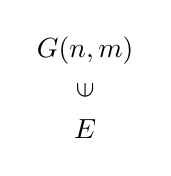
\begin{tikzpicture}
\node at (0,0) {\(G(n,m)\)};
\node[rotate=90] at (0,-.5) {\(\in\)};
\node at (0,-1) {\(E\)};
\end{tikzpicture}}\endgroup}\par\smallskip}
\end{GelfandAdjacentEvidence}
\begin{GelfandAdjacentEvidence}{GELFAND-P001229}{3}

\(e_1,\ldots,e_n\) --- базис в \(\mathbb R^n\)
\begin{equation*}
\tau_E=(Pe_1,\ldots,Pe_n)
\end{equation*}
Какова топ. страта в \(G(n,m)\), где \(\tau_E\) имеет заданный комбинат. тип?

\(2^{\circ}.\) Комбинат. теория выпуклых многогранников в \(\mathbb R^n\).

2 многогранника \(V_1,V_2\) с упорядоч. (занумер.) вершинами (\(n\) штук)
[зачёркнуто] имеют одинак. комбинат. тип, если грани соответствуют друг другу.
\Incomplete{GELFAND-P001229}{cancelled-type}{Зачёркнутый фрагмент после «\(n\) штук» не разобран.}
\end{GelfandAdjacentEvidence}
\begin{GelfandAdjacentEvidence}{GELFAND-P001229}{4}


Грассманизация задачи.

В \(\mathbb R^n\) рассм. подпр-во (\(m\)-мерное) \(E\)
\begin{equation*}
S=\omega(e_1,\ldots,e_n)\quad\text{--- симплекс}
\end{equation*}
\EvidenceBlock{GELFAND-P001229}{simplex-symbol}{После знака равенства написано \(\omega\).}{Запись в рукописи.}
\end{GelfandAdjacentEvidence}
\begin{GelfandAdjacentEvidence}{GELFAND-P001229}{5}

Проекция \(S\) на \(E\) --- многогранник (выпуклый)

\underline{Упр.:} получ. комбинаторно любой многогранник разм. \(m\) с \(n\) вершинами

На \(G(n,m)\) рассм. разбиение на подмн-ва, где несомые подпр-вом многогранники комбинаторно эквивалентны.
\EvidenceBlock{GELFAND-P001229}{subspace-abbreviation}{После «несомые» написано «подпр-вом».}{Запись в рукописи.}
\end{GelfandAdjacentEvidence}
\begin{GelfandAdjacentEvidence}{GELFAND-P001229}{6}


Какова топология этих кусков?

\(3^{\circ}.\)
\SourceFigure{GELFAND-P001229}{matrix-hatching}{%
\par\smallskip
{\color{black}\(\begin{array}{c}
\left(\begin{array}{@{}ccc@{}}
x_{11}&\cdots&x_{1n}\\
x_{21}&\cdots&x_{2n}\\
x_{31}&\cdots&x_{3n}\\
\hline
\multicolumn{3}{c}{\text{\tikz[x=.65cm,y=.40cm]{
\draw (0,.02)--(.37,.26)--(.24,.04)--(.74,.24)--(.61,.02)--(1.13,.24)--(1.00,.03)--(1.54,.22)--(1.39,.01)--(1.89,.23);}}}
\end{array}\right)
\qquad
\begin{pmatrix}
x'_{11}&\cdots&x'_{1n}\\
x'_{21}&\cdots&x'_{2n}\\
x'_{31}&\cdots&x'_{3n}
\end{pmatrix}\\[3pt]
\text{--- 2 матрицы }3\times n
\end{array}\)}\par\smallskip
Под третьей строкой первой матрицы черта и петлеобразная штриховка. Назначение штриховки неясно. Во второй матрице этих помет нет.}
\end{GelfandAdjacentEvidence}


Пусть все миноры \(\ne0\) и имеют одинаковые знаки для \(x\) и \(x'\).

Сущ. ли гомотопия \(x(t)\) матриц с \(x(0)=x\), \(x(1)=x'\)


\Needspace{7\baselineskip}
\begin{GelfandAdjacentEvidence}{GELFAND-P001230}{1}
\SourcePage{GELFAND-P001230}{15}
в этом же классе?
\begin{gather*}
n\le7\ \Rightarrow\ \text{можно}\\
n=19\ \Rightarrow\ \text{нельзя!}\qquad\text{(Н.Е. Мнёв)}
\end{gather*}
Конфигурации имеют смысл и в \(\mathbb RP^n\) и нужно дополнять.
\EvidenceBlock{GELFAND-P001230}{configuration-end}{Последнее слово читается «дополнять».}{Запись в рукописи.}
\end{GelfandAdjacentEvidence}
\begin{GelfandAdjacentEvidence}{GELFAND-P001230}{2}


Надо [пощупать?] следствия (проектированием) и есть оценка, сколько их надо брать, чтобы было достаточно.
\Unclear{GELFAND-P001230}{consequences-verb}{Соединённые штрихи допускают предположительное чтение «пощупать». Следующее слово «следствия» читается отчётливо.}
\end{GelfandAdjacentEvidence}
\begin{GelfandAdjacentEvidence}{GELFAND-P001230}{3}

\EvidenceBlock{GELFAND-P001230}{consequences-parenthesis}{В скобках написано «проектированием». Далее написано «и есть оценка».}{Запись в рукописи.}
\end{GelfandAdjacentEvidence}
\begin{GelfandAdjacentEvidence}{GELFAND-P001230}{4}


Топология может быть как у любого алгебр. мн-зия!

(Это над \(\mathbb R\))

над \(C\) аналогом является вычисление \(\pi_1\).

Интересно, что является выпуклым аналогом над \(C\).

\underline{Теор. Стейница}: характеризация 1-мерн. остова вып. многогранника

(см. любой учебник вып. геом.) (в \(\mathbb R^3\))

\underline{Следствие}: пр-во многогр. данного комбинат. типа в \(\mathbb R^3\) стягиваемо.

\underline{Но}: в \(\mathbb R^4\) уже сущ. даже уже симплициальные многогранники
с более или менее любой [зачёркнуто] топологией комбинат. типа.
\Incomplete{GELFAND-P001230}{topology-cancel}{Слово между «любой» и «топологией» зачёркнуто и не разобрано.}
\end{GelfandAdjacentEvidence}
\begin{GelfandAdjacentEvidence}{GELFAND-P001230}{5}


\uwave{Задача}: хотим на мн-зии построить поле многогранников! (в каждом кас. пр-ве).
Была [зачёркнуто] классифик. задача для этой.
\Incomplete{GELFAND-P001230}{classification-cancel}{После «Была» зачёркнута неразобранная запись.}
\end{GelfandAdjacentEvidence}
\begin{GelfandAdjacentEvidence}{GELFAND-P001230}{6}


\uwave{Матроиды} [м.?] Дана решётка. Она наз. \uwave{геометрич. решёткой},
если она
\begin{enumerate}
\item[1)] Полумодулярна
\item[2)] Конечная (\(\forall\) элемент \(=\sup\) конечн. числа атомов)
\end{enumerate}
[Под этой строкой:] атомы --- след. за нулём.
\Unclear{GELFAND-P001230}{matroid-mark}{Переправленный знак после «Матроиды» предположительно читается «м.». Назначение пометы неясно.}
\end{GelfandAdjacentEvidence}
\begin{GelfandAdjacentEvidence}{GELFAND-P001230}{7}


Конфигур. --- геом. решётка.

Обратно, пусть дана геом. решётка. Когда она зад. конфигур.?

\SourceFigure{GELFAND-P001230}{fano-diagram}{%
\par\smallskip
{\color{black}\begingroup\color{black}\GelfandFitDiagram{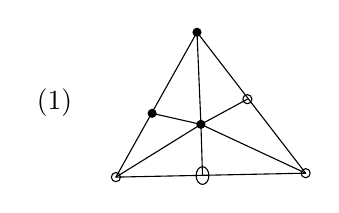
\begin{tikzpicture}[x=1cm,y=1cm,line cap=round,line join=round]
\coordinate (T) at (1.03,1.84);
\coordinate (L) at (0,0);
\coordinate (R) at (2.41,.05);
\coordinate (TL) at (.46,.81);
\coordinate (TR) at (1.67,.99);
\coordinate (B) at (1.1,.02);
\coordinate (C) at (1.08,.67);
\node[anchor=east] at (-.43,.95) {(1)};
\draw (L)--(T)--(R)--cycle;
\draw (T)--(C)--(B) (L)--(C)--(TR) (R)--(C)--(TL);
\foreach \point in {T,TL,C} \fill (\point) circle[radius=1.65pt];
\foreach \point in {L,R,TR} \draw (\point) circle[radius=1.65pt]; \draw (B) ellipse[x radius=2.3pt,y radius=3.2pt];
\end{tikzpicture}}\endgroup}\par\smallskip
Видно семь отмеченных точек и три внутренние линии. Нижняя средняя петля выступает под основание. Отдельной линии через три точки на сторонах не видно.}
\end{GelfandAdjacentEvidence}
\begin{GelfandAdjacentEvidence}{GELFAND-P001230}{8}

(конфигур. Фано)\qquad над \(\mathbb R,\mathbb Z\) не реализуется.

Верное предст. решётки \(=\) её отображение
\begin{equation*}
a:\Gamma\longrightarrow\mathcal L(F^n)\quad\text{--- реш. подпр-в,}
\end{equation*}
такое что
\begin{equation*}
\gamma_1<\gamma_2\ \Rightarrow\ a(\gamma_1)<a(\gamma_2)
\end{equation*}
и \(\sup\) сохраняется

(1) не реализуется [зачёркнуто] над \(\mathbb R\), но над \(\mathbb Z_2\) реализу..
\Unclear{GELFAND-P001230}{realization-cancel}{Знак перед «над» зачёркнут и не разобран.}
\end{GelfandAdjacentEvidence}



\Needspace{7\baselineskip}
\begin{GelfandAdjacentEvidence}{GELFAND-P001231}{1}
\SourcePage{GELFAND-P001231}{unlabelled}
Верное предст. есть у конфигур. (1):
\begin{equation*}
?\qquad m=4,\quad E,\quad \underline F,\quad \underline{\mathbb R^6}
\end{equation*}
\EvidenceBlock{GELFAND-P001231}{opening-symbols}{В строке с вопросительным знаком отдельно записаны \(m=4\), \(E\), \(F\) и \(\mathbb R^6\).}{Запись в рукописи.}
\end{GelfandAdjacentEvidence}
\begin{GelfandAdjacentEvidence}{GELFAND-P001231}{2}


Зад. о реализуемости \(\Leftrightarrow\) зад. о реш. системы алгебраических нер-в.
\EvidenceBlock{GELFAND-P001231}{inequalities-reading}{После «алгебраических» написано «нер-в.» (неравенств).}{Запись в рукописи.}
\end{GelfandAdjacentEvidence}
\begin{GelfandAdjacentEvidence}{GELFAND-P001231}{3}


\uwave{Нетрив. раб. по структурам:} (по Гельфанду)
\EvidenceBlock{GELFAND-P001231}{lattice-heading}{Первое сокращение в заголовке читается «Нетрив.».}{Запись в рукописи.}
\end{GelfandAdjacentEvidence}
\begin{GelfandAdjacentEvidence}{GELFAND-P001231}{4}


Дедекинд: придумал

Курош, Оре.

фон Нейман;

Гельфанд, Пономарёв:

[На левом поле: \uwave{Доб. Вершика:}]
\uwave{Пудлак и Тум} (Чехи): всякая конечная решётка вкладывается в решётку разбиений конечного мн-ва (очень трудная теорема).

(\(\inf\) и \(\sup\) --- [зачёркнуто] пересеч. и объед.)
\Incomplete{GELFAND-P001231}{inf-sup-cancel}{Слово после «inf и sup» зачёркнуто и не разобрано.}
\end{GelfandAdjacentEvidence}
\begin{GelfandAdjacentEvidence}{GELFAND-P001231}{5}


\(0\) --- разб. на точки.

\medskip
\underline{\underline{Фейгин Б.}}\qquad\underline{О струнах} [зачёркнуто] (продолжение).
\Unclear{GELFAND-P001231}{string-heading-cancel}{Вертикальный зачёркнутый знак после «О струнах» не разобран.}
\end{GelfandAdjacentEvidence}
\begin{GelfandAdjacentEvidence}{GELFAND-P001231}{6}


\underline{Операторная теория струн.}

\underline{Дуальные амплитуды.} Рассм. столкновение частиц

\SourceFigure{GELFAND-P001231}{scattering-diagram}{%
\par\smallskip
{\color{black}\begingroup\color{black}\GelfandFitDiagram{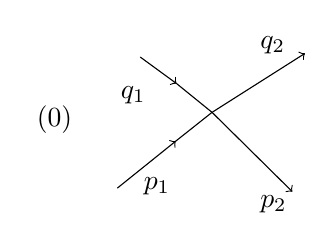
\begin{tikzpicture}[x=1cm,y=.96cm,line cap=round]
\node at (-2,0) {(0)};
\coordinate (lowerin) at (-1.2,-.90);
\coordinate (upperin) at (-.91,.83);
\coordinate (crossing) at (0,.10);
\coordinate (upperout) at (1.18,.88);
\coordinate (lowerout) at (1.02,-.95);
\draw[->] (lowerin)--(-.46,-.28);
\draw[->] (-.46,-.28)--(crossing)--(upperout);
\draw[->] (upperin)--(-.45,.48);
\draw[->] (-.45,.48)--(crossing)--(lowerout);
\node[below] at (-.70,-.63) {\(p_1\)};
\node[left] at (-.72,.33) {\(q_1\)};
\node[above] at (.77,.74) {\(q_2\)};
\node[below] at (.78,-.87) {\(p_2\)};
\end{tikzpicture}}\endgroup}\par\smallskip}
\end{GelfandAdjacentEvidence}
\begin{GelfandAdjacentEvidence}{GELFAND-P001231}{7}


Массы пусть все одинаковы и полный импульс \(=0\)

Всё --- векторы в пр-ве/времени
\begin{equation*}
\begin{cases}
p_1+q_1=p_2+q_2,\\
p_1^2=q_1^2=p_2^2=q_2^2=m^2
\end{cases}
\qquad p_j,q_j\in\mathbb R^4.
\tag{1}
\end{equation*}
\EvidenceBlock{GELFAND-P001231}{mass-shell-overwrite}{Переправленная буква с индексом в предпоследнем квадрате читается \(q_2\).}{Запись в рукописи.}
\end{GelfandAdjacentEvidence}
\begin{GelfandAdjacentEvidence}{GELFAND-P001231}{8}


Пусть дана \(S\)-матрица, характериз. это столкновение,
\begin{equation*}
S(p_1,q_1,p_2,q_2)\tag{2}
\end{equation*}
Переменные Мандельстама:
\begin{equation*}
\begin{cases}
s=(p_1+q_1)^2,\\
t=(p_1-p_2)^2\\
u\ \text{[зачёркнуто]}=(p_1-q_2)^2
\end{cases}\tag{3}
\end{equation*}
\Unclear{GELFAND-P001231}{mandelstam-u-cancel}{После \(u\) перед равенством зачёркнут неразобранный знак.}
\end{GelfandAdjacentEvidence}
\begin{GelfandAdjacentEvidence}{GELFAND-P001231}{9}

[Справа от (3):] (Заданы релятивистски инвариантные попарные скал. произведения)

зависимы:
\begin{equation*}
s+t+u=4m^2\tag{4}
\end{equation*}
Зададим \(A(s,t)\) (\(=\) выражение \(S\) через \(s,t\))

\uwave{Требование}:
\begin{equation*}
1)\quad A\text{ аналитична по }s,t\quad\text{[зачёркнуто]}\tag{5}
\end{equation*}
\Unclear{GELFAND-P001231}{analytic-tail}{После \(t\) зачёркнут знак. Его чтение не установлено.}
\end{GelfandAdjacentEvidence}



\Needspace{7\baselineskip}
\begin{GelfandAdjacentEvidence}{GELFAND-P001232}{1}
\SourcePage{GELFAND-P001232}{16}
2) \(A\) симметрична по \(s,t\) (независ. от порядка)

3) При фиксир. \(t\) ф-я \(A(s,t)\) имеет по \(s\) только простые полюса,
причём [вписано между словами: 4)] места полюсов не зависят от \(t\). Обычно пишут:
\begin{equation*}
A(s,t)=\sum_{n=0}^{\infty}\frac{R_n(t)}{n-\alpha(s)}\tag{6}
\end{equation*}
5) \(R_n(t)\) --- многочлен

График \(\alpha(s)\) наз. траекторией Редже.

Оказ., что из 1)---5) однозначно находим вид ф-и \(A\):
\begin{equation*}
A(s,t)=\frac{\Gamma(-\alpha(s))\Gamma(-\alpha(t))}{\Gamma(-\alpha(s)-\alpha(t))}
=B(-\alpha(s),-\alpha(t))\tag{7}
\end{equation*}
Из анализа экспер. данных вытекает, что
\begin{equation*}
\alpha(s)\quad\text{--- линейная ф-я}\tag{8}
\end{equation*}
\(A\) наз. амплитудой Венециано, или дуальной амплитудой, а усл. 1)---5) наз. \underline{условиями дуальности}.

Операторный метод: хотим записать \(A(s,t)\) как опер. среднее
\begin{equation*}
\langle0|V(t)V(s)|0\rangle,\tag{9}
\end{equation*}
где \(\langle0|\) --- вак. вектор в каком-то пр-ве, \(V(t)\) --- операторы.

Другая запись (7):
\begin{equation*}
S(p_1,p_2,p_3,p_4)=\int_0^1
x^{-2\langle p_1,p_2\rangle}(1-x)^{-2\langle p_2,p_3\rangle}
(x(1-x))^{-1-m^2}\,dx\tag{10}
\end{equation*}
Здесь

\SourceFigure{GELFAND-P001232}{amplitude-arrow-convention}{%
\par\smallskip
{\color{black}\begingroup\color{black}\GelfandFitDiagram{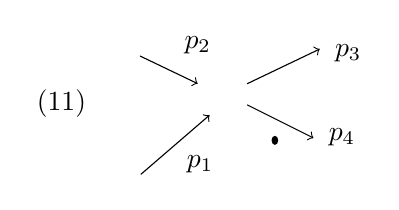
\begin{tikzpicture}[x=1cm,y=1cm,line cap=round]
\node at (-2.1,0) {(11)};
\draw[->] (-1.1,.60)--(-.37,.25);
\draw[->] (-1.09,-.90)--(-.22,-.15);
\draw[->] (.26,.25)--(1.18,.69);
\draw[->] (.26,-.02)--(1.1,-.44);
\node[above] at (-.37,.50) {\(p_2\)};
\node[below] at (-.34,-.54) {\(p_1\)};
\node[right] at (1.25,.64) {\(p_3\)};
\node[right] at (1.17,-.43) {\(p_4\)};
\fill (.61,-.47) ellipse[x radius=1.2pt,y radius=1.65pt];
\end{tikzpicture}}\endgroup}\par\smallskip
Рядом с нижней правой стрелкой виден чернильный след. Его связь со стрелкой неясна.}
\end{GelfandAdjacentEvidence}
\begin{GelfandAdjacentEvidence}{GELFAND-P001232}{2}

\begin{equation*}
p_1+p_2+p_3+p_4=0.
\end{equation*}
Аналогично можно писать амплитуды для большего числа частиц,
например:
\begin{equation*}
A(p_1,p_2,p_3,p_4,p_5)\cong\int\int_0^1
x^{\cdots}y^{\cdots}(1-x)^{\cdots}(1-y)^{\cdots}(1-xy)^{\cdots}\,dx\,dy\tag{12}
\end{equation*}
Эта амплитуда уже не вычислена в общем виде, только при нек-рых спец. значениях \underline{скал. произведений}.

Пр-во порождено конечным набором осцилляторов, к-рые соед. как в струне. Конечным числом обойтись нельзя!.
\EvidenceBlock{GELFAND-P001232}{finite-oscillators}{В первом предложении написано «конечным», во втором --- «Конечным числом обойтись нельзя!».}{Запись в рукописи.}
\end{GelfandAdjacentEvidence}
\begin{GelfandAdjacentEvidence}{GELFAND-P001232}{3}


Рассм. алгебру с образующими
\begin{equation*}
a_m^\mu,x^\mu,\quad \mu=0,1,\ldots,d,\quad
\text{[зачёркнуто]}\tag{13}
\end{equation*}
\Incomplete{GELFAND-P001232}{generators-cancel}{Запись после \(d\) в (13) зачёркнута и не разобрана.}
\end{GelfandAdjacentEvidence}

где \(d\) --- разм. пр-ва


\Needspace{7\baselineskip}
\begin{GelfandAdjacentEvidence}{GELFAND-P001233}{1}
\SourcePage{GELFAND-P001233}{unlabelled}
\begin{equation*}
\relax [a_m^\mu,a_n^\nu]=m g^{\mu\nu}\delta_{m,-n}\tag{14}
\end{equation*}
\(m,n\) --- целые числа
\begin{equation*}
a_0^\mu=p^\mu\tag{15}
\end{equation*}
\begin{equation*}
\relax [x^\mu,p^\nu]=i g^{\mu\nu}\tag{16}
\end{equation*}
\EvidenceBlock{GELFAND-P001233}{momentum-superscript}{Переправленный верхний индекс у \(p\) в (16) читается \(\nu\).}{Запись в рукописи.}
\end{GelfandAdjacentEvidence}
\begin{GelfandAdjacentEvidence}{GELFAND-P001233}{2}

\begin{equation*}
\relax [x^\mu,a_m^\nu]=0,\quad m\ne0\tag{17}
\end{equation*}
Смысл образующих \(x^\mu,a_m^\mu\):

[Зачёркнуто: \(p^\mu\) --- не разобрано]
\Unclear{GELFAND-P001233}{coordinates-cancel}{В начале зачёркнутой записи читается \(p^\mu\). Остальные знаки неразборчивы.}
\end{GelfandAdjacentEvidence}
\begin{GelfandAdjacentEvidence}{GELFAND-P001233}{3}

\((x^\mu,p^\mu)\) --- коорд. и импульс центра тяжести летящей струны, \(a_m^\mu\) --- разлож. в ряд Фурье всего остального.

Положим:
\begin{equation*}
P^\mu(\theta)=\sum_{-\infty}^{+\infty}a_m^\mu e^{-im\theta},\tag{18}
\end{equation*}
(импульс точки с парам. \(\theta\))
\begin{equation*}
Q^\mu(\theta)=x^\mu+a_0^\mu\theta+
 i\sum_{\substack{n=-\infty\\n\ne0}}^{\infty}\frac1n a_{[m?]}^\mu e^{-in\theta}.\tag{19}
\end{equation*}
\Unclear{GELFAND-P001233}{fourier-index}{Переправленный нижний индекс при \(a\) предположительно читается \(m\), возможно \(n\). В сумме и показателе экспоненты написано \(n\).}
\end{GelfandAdjacentEvidence}
\begin{GelfandAdjacentEvidence}{GELFAND-P001233}{4}

Тогда выполнены коммутационные соотношения:
\begin{equation*}
\relax [Q_\mu(\theta),P_\nu(\theta')]=2\pi i g_{\mu\nu}\delta(\theta-\theta')\tag{20}
\end{equation*}
\begin{equation*}
\relax [P_\mu(\theta),P_\nu(\theta')]=2\pi i g_{\mu\nu}\delta'(\theta-\theta')\tag{21}
\end{equation*}
\begin{equation*}
\relax [Q_\mu(\theta),Q_\nu(\theta')]=-\pi i g_{\mu\nu}\varepsilon(\theta-\theta'),\tag{22}
\end{equation*}
где \(\varepsilon\) --- ф-я Хевисайда
\Unclear{GELFAND-P001233}{heaviside-convention}{Написано «где \(\varepsilon\) --- ф-я Хевисайда». Нормировка здесь не указана.}
\end{GelfandAdjacentEvidence}
\begin{GelfandAdjacentEvidence}{GELFAND-P001233}{5}

\begin{equation*}
L_m\overset{\mathrm{def}}{=}\frac1{4\pi}\int_0^{2\pi}
e^{im\theta}:P^2(\theta):\,d\theta\tag{23}
\end{equation*}
Тогда получ. представление алгебры Вирасоро
\begin{equation*}
\relax [L_m,L_n]=(m-n)L_{m+n}+\frac d{12}(m^3-m)\delta_{m,-n}\tag{24}
\end{equation*}
\Unclear{GELFAND-P001233}{central-dimension}{Коэффициент центрального члена написан \(\frac{d}{12}\).}
\end{GelfandAdjacentEvidence}


\uwave{Упражнение}: проверить это.

Кстати,
\begin{equation*}
L_0=\frac12a_0^2+\sum_{n=1}^{\infty}a_{-n}a_n\tag{25}
\end{equation*}


\Needspace{7\baselineskip}
\begin{GelfandAdjacentEvidence}{GELFAND-P001234}{1}
\SourcePage{GELFAND-P001234}{17}
\begin{equation*}
2L_m={:}\sum_{r+s=m}a_ra_s{:}\tag{26}
\end{equation*}
\uwave{Вертексный оператор}: положим
\begin{equation*}
V(k,\theta)=\exp\langle ik,Q(\theta)\rangle,\tag{27}
\end{equation*}
где \(k\) --- вектор, тогда
\begin{equation*}
V(k)=V(k,0)=
\exp\left\langle k,\sum_{n=1}^{\infty}\frac{a_{-n}}n\right\rangle
\exp(ikx)
\exp\left\langle-k,\sum_{n=1}^{\infty}\frac{a_n}n\right\rangle
\tag{28}
\end{equation*}
\EvidenceBlock{GELFAND-P001234}{vertex-insertion}{Множитель \(\exp(ikx)\) вписан над строкой. Линии от вставки сходятся между двумя экспонентами.}{Запись в рукописи.}
\end{GelfandAdjacentEvidence}
\begin{GelfandAdjacentEvidence}{GELFAND-P001234}{2}

и
\begin{equation*}
V(k,\theta)=\exp(i\theta L_0)V(k)\exp(-i\theta L_0).\tag{29}
\end{equation*}
Далее,

[Зачёркнуто перед (30)]
\begin{equation*}
\relax [L_n-L_0,V(k)]=\frac{nk^2}2V(k).\tag{30}
\end{equation*}
\Incomplete{GELFAND-P001234}{commutator-cancel}{Запись перед коммутатором (30) зачёркнута и не разобрана.}
\end{GelfandAdjacentEvidence}
\begin{GelfandAdjacentEvidence}{GELFAND-P001234}{3}


Рассмотрим серию взаимодействий:

\SourceFigure{GELFAND-P001234}{interaction-chain}{%
\par\smallskip
{\color{black}\begingroup\color{black}\GelfandFitDiagram{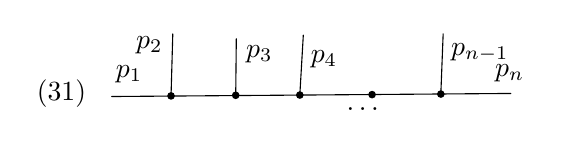
\begin{tikzpicture}[x=.74cm,y=.78cm,line cap=round]
\node at (-.86,.05) {(31)};
\draw (0,0)--(6.85,.05);
\draw (1.02,.01)--(1.05,1.02) (2.13,.02)--(2.14,.94)
      (3.23,.024)--(3.29,1.0) (5.65,.04)--(5.69,1.02);
\foreach \x/\y in {1.02/.01,2.13/.02,3.23/.024,4.47/.031,5.65/.04}
   \fill (\x,\y) circle[radius=1.38pt];
\node[above] at (.30,.06) {\(p_1\)};
\node[left] at (1.04,.83) {\(p_2\)};
\node[right] at (2.14,.69) {\(p_3\)};
\node[right] at (3.25,.61) {\(p_4\)};
\node[right] at (5.66,.72) {\(p_{n-1}\)};
\node[above] at (6.83,.08) {\(p_n\)};
\node[below] at (4.31,-.02) {\(\ldots\)};
\end{tikzpicture}}\endgroup}\par\smallskip}
\end{GelfandAdjacentEvidence}
\begin{GelfandAdjacentEvidence}{GELFAND-P001234}{4}


и по такой картинке построим амплитуду:
\begin{equation*}
\langle0|V(p_2)D(s_2)V(p_3)D(s_3)\ldots D(s_{n-2})V(p_{n-1})|0\rangle,
\tag{32}
\end{equation*}
\EvidenceBlock{GELFAND-P001234}{last-propagator-index}{Переправленная цифра в последнем аргументе \(D\) читается \(2\). Написано \(s_{n-2}\).}{Запись в рукописи.}
\end{GelfandAdjacentEvidence}

где \(p\) --- то же самое, что и \(k\),
\begin{equation*}
\begin{aligned}
s_2&=(p_2+p_1)^2\\
s_3&=(p_3+p_2+p_1)^2,\\
&\ldots
\end{aligned}\tag{33}
\end{equation*}
\begin{equation*}
D(s)=\int_0^1 x^{L_0-\alpha(s)-1}(1-x)^{\alpha(0)-1}\,dx,\tag{34}
\end{equation*}
где \(\alpha(s)\) --- линейная ф-я (траектория Редже).

(32) --- дуальная амплитуда; она должна совпадать с \(A\), когда 4 вершины.

Разложим \(V(k,\theta)\) в ряд Фурье:
\begin{equation*}
V(k,\theta)=\sum V_n(k)e^{-in\theta}.\tag{35}
\end{equation*}
Имеются операторы \(a_i^\mu\) и \(a_0^\mu\) и вакуумные векторы
\(|0,p\rangle\), удовлетв. условию


\Needspace{7\baselineskip}
\begin{GelfandAdjacentEvidence}{GELFAND-P001235}{1}
\SourcePage{GELFAND-P001235}{unlabelled}
\begin{equation*}
a_i^\mu|0,p\rangle=0,\quad\text{если }i>0,
\tag*{$(36)_i$}
\end{equation*}
\begin{equation*}
a_0^\mu|0,p\rangle=
\text{[зачёркнуто]}\ p^\mu\,\text{[зачёркнуто]}\ |0,p\rangle.
\tag*{$(36)_0$}
\end{equation*}
\Unclear{GELFAND-P001235}{vacuum-cancel-left}{зачёркнутая запись перед $p^\mu$}
\end{GelfandAdjacentEvidence}
\begin{GelfandAdjacentEvidence}{GELFAND-P001235}{2}

\Unclear{GELFAND-P001235}{vacuum-cancel-right}{зачёркнутый знак после $p^\mu$}
\end{GelfandAdjacentEvidence}
\begin{GelfandAdjacentEvidence}{GELFAND-P001235}{3}

(вакуумы занумерованы векторами импульса)

Получим пр-во
\begin{equation*}
\bigoplus_p H(p)
\tag{37}
\end{equation*}
Вертексный оператор действует так:
\begin{equation*}
V_n(k):H(p)\longrightarrow H(p+k).
\tag{38}
\end{equation*}
Коммутационные соотношения:

[Зачёркнуто: неразборчиво]
\Incomplete{GELFAND-P001235}{commutator-cancel}{Зачёркнутая запись под заголовком «Коммутационные соотношения» не прочитана.}
\end{GelfandAdjacentEvidence}
\begin{GelfandAdjacentEvidence}{GELFAND-P001235}{4}

\begin{equation*}
\relax [a_m^\mu,V_n(k)]=V_{n+m}(k)\cdot k_\mu
\tag{39}
\end{equation*}
\EvidenceBlock{GELFAND-P001235}{commutator-index}{В множителе \(k_\mu\) в (39) индекс \(\mu\) написан внизу.}{Запись в рукописи.}
\end{GelfandAdjacentEvidence}
\begin{GelfandAdjacentEvidence}{GELFAND-P001235}{5}


[Зачёркнуто: $V_n(k_1)|0,p\rangle$ / $V_1(k_1)|0,p\rangle$\textsuperscript{?}] Положим
\Unclear{GELFAND-P001235}{vertex-cancel}{В зачёркнутой записи читаются \(V\), \((k_1)\) и \(\lvert 0,p\rangle\). Нижний индекс \(V\) предположительно \(n\) или \(1\).}
\end{GelfandAdjacentEvidence}
\begin{GelfandAdjacentEvidence}{GELFAND-P001235}{6}

\begin{equation*}
\langle0,p+k_1+k|V_{-n}(k_2)V_n(k_1)|0,p\rangle=A_n\qquad\text{(это числа)}
\tag{40}
\end{equation*}
\EvidenceBlock{GELFAND-P001235}{bra-last-momentum}{В бра-векторе (40) написано \(p+k_1+k\). У последнего \(k\) нет нижнего индекса.}{Запись в рукописи.}
\end{GelfandAdjacentEvidence}


Тогда
\begin{equation*}
\sum A_n z^n=(1-z)^{\langle k_1,k_2\rangle}.
\tag{41}
\end{equation*}
Это доказывается простым вычислением. Предлагается проверить (41) в качестве упражнения.


\Needspace{7\baselineskip}
\begin{GelfandAdjacentEvidence}{GELFAND-P001236}{1}
\SourcePage{GELFAND-P001236}{26}
\underline{18/XI–85г.}\qquad \underline{Сем. Гельфанда}

\underline{Б. Фейгин} (продолжение).

$L_i$ — образующие алг. Вирасоро; пусть есть большое пр-во, в к-ром действ. эта алгебра

Соб. векторы $L_0=$ весовые векторы

$L_i$ действует в пр-ве весовых векторов из коммут. соотношений

(см. (24) на стр. 17 лев.)

Старший [зачёркнуто: вектор?\textsuperscript{?}] вес: вектор, к-рый нельзя уже повысить
\Unclear{GELFAND-P001236}{highest-cancel}{Зачёркнутое слово предположительно читается «вектор». Середина слова перекрыта штрихами.}
\end{GelfandAdjacentEvidence}
\begin{GelfandAdjacentEvidence}{GELFAND-P001236}{2}

\begin{equation*}
\widetilde{\mathcal H}=\{v\mid L_0v=v,\quad L_iv=0\ \text{при }i>0\}.\qquad\text{(вес 1)}
\tag{1}
\end{equation*}
\begin{equation*}
\overline{\mathcal H}=\{v\in\widetilde{\mathcal H},\quad v=L_i v',\ i<0\},
\tag{2}
\end{equation*}
[Справа:] здесь $v'$ — произв. весовой вектор из большого пр-ва.

(пр-во «спурионов» — назв. физиков, $\sim15$ лет назад)
\begin{equation*}
\mathcal H\overset{\mathrm{def}}{=}\widetilde{\mathcal H}/\overline{\mathcal H}
\tag{3}
\end{equation*}
\begin{equation*}
\prod_{i=1}^N a_{m_i}^{\mu_i}|0,p\rangle
\tag{4}
\end{equation*}
[Справа:] (пр-во состояний)

большой модуль над алг. Вирасоро
\begin{equation*}
L_{-1}v'=v\quad\Rightarrow\quad v'\text{ имеет вес }2:\quad L_0v'=2v'
\tag{5}
\end{equation*}
\EvidenceBlock{GELFAND-P001236}{weight-two}{В (5) написано \(L_{-1}v'=v\), «\(v'\) имеет вес 2» и \(L_0v'=2v'\).}{Запись в рукописи.}
\end{GelfandAdjacentEvidence}
\begin{GelfandAdjacentEvidence}{GELFAND-P001236}{3}


Цель: факторизация отн. группы диффеом. во всём пр-ве, но действует центр. расширение, и центр действ. нетривиально.

Предлаг. другая процедура получ. «инвар.» векторов: относит. половины они инвар., затем факторизуем по действию других и отбрасываем.

Алг. Вирасоро исчезает, от неё остаётся пр-во инвариантов.

Хотим:

I. Построить пр-во, порожд. $d-2$ осцилляторами.

II. Док., что все векторы в $\widetilde{\mathcal H}/\overline{\mathcal H}$ имеют норму $>0$

(в исх. $d$-мерном это не так)

(отсутствие \underline{тахионов\textsuperscript{?}})
\EvidenceBlock{GELFAND-P001236}{tachyon-word}{Подчёркнутое слово читается «тахионов».}{Запись в рукописи.}
\end{GelfandAdjacentEvidence}


В размерности 26 это всё достигается.


\Needspace{7\baselineskip}
\begin{GelfandAdjacentEvidence}{GELFAND-P001237}{1}
\SourcePage{GELFAND-P001237}{unlabelled}
Вертексные операторы:
\begin{equation*}
X(p,z)=\exp\left(p_\mu\cdot\sum_{n=1}^{\infty}a_{-n}^\mu z^n\right)D_p
\exp\left(-p_\mu\sum_{n=1}^{\infty}\frac{a_n^\mu}{n}z^{-n}\right),
\tag{6}
\end{equation*}
\EvidenceBlock{GELFAND-P001237}{left-exponential-normalization}{В левой экспоненте (6) написано \(a_{-n}^{\mu}z^n\) без дробной черты и знаменателя.}{Запись в рукописи.}
\end{GelfandAdjacentEvidence}
\begin{GelfandAdjacentEvidence}{GELFAND-P001237}{2}


где операторы $D_p$ опред. ф-лами
\begin{equation*}
D_p|0,k\rangle=|0,k+p\rangle,\quad [D_p,a_n^\mu]=0,\ n\ne0.
\tag{7}
\end{equation*}
Корреляционная функция:
\begin{equation*}
\begin{aligned}
&\langle0,k+\textstyle\sum p_i|X(z_1,p_1)\ldots X(z_n,p_n)|0,k\rangle\\
&\qquad=\prod_{j>1}\left(1-\frac{z_j}{z_i}\right)^{\langle p_i,p_j\rangle}.
\end{aligned}
\tag{8}
\end{equation*}
\EvidenceBlock{GELFAND-P001237}{product-index}{Под знаком произведения написано \(j>1\). Последний знак имеет нижнюю ножку цифры \(1\).}{Запись в рукописи.}
\end{GelfandAdjacentEvidence}
\begin{GelfandAdjacentEvidence}{GELFAND-P001237}{3}


Разлагая $X(z,p)$ в ряд, получим:
\begin{equation*}
X(z,p)=\sum X_i(p)z^i
\tag{9}
\end{equation*}
(это определение операторов $X_i(p)$)

Хотим построить 24 осциллятора.

Далее будут строиться операторы
\begin{equation*}
\int X(p,z)\frac{dz}{z},
\tag{10}
\end{equation*}
коммутирующие с алг. Вирасоро при $\langle p,p\rangle=2$.
\begin{equation*}
\begin{aligned}
&\text{На }\mathbb R^{26}\text{ хотим иметь }p_1,\ldots,p_n:\quad\langle p_i,p_i\rangle=2\\
&\langle p_i,p_j\rangle=A_{ij}\in\mathbb Z,\quad A_{ij}<0.
\end{aligned}
\tag{11}
\end{equation*}
[На левом поле: зачёркнутый вертикальный знак\textsuperscript{?}]
\Unclear{GELFAND-P001237}{cartan-margin-cancel}{зачёркнутый вертикальный знак}
\end{GelfandAdjacentEvidence}
\begin{GelfandAdjacentEvidence}{GELFAND-P001237}{4}


\EvidenceBlock{GELFAND-P001237}{cartan-diagonal}{Написано \(A_{ij}<0\). Рядом с неравенством нет ограничения на индексы.}{Запись в рукописи.}
\end{GelfandAdjacentEvidence}


Тогда операторы
\begin{equation*}
e_i=\int X(p_i,z)\frac{dz}{z},\quad f_i=\int X(-p_i,z)\frac{dz}{z}
\tag{12}
\end{equation*}
порождают на пр-ве действие алгебры Каца–Муди с матрицей Картана $A_{ij}$; при этом надо ещё положить
\begin{equation*}
h_i|0,k\rangle=\langle k,p_i\rangle|0,k\rangle
\tag{13}
\end{equation*}
\underline{Читать}: \underline{ст. МакДональда} (начало), \underline{Sem. Bourbaki};

учить алгебры Ли по ней.

[На левом поле: И.М.Г.] В самой большой простой конечной группе $\sim10^{54}$ элементов; она связана со струнами!

[Приписано справа:] (монстр «Лунное сияние»)

Moonshine

(есть раб. Френкель, Леповский и кто-то ещё)

Как-то получ. фунд. предст. алг. Каца–Муди.


\Needspace{7\baselineskip}
\begin{GelfandAdjacentEvidence}{GELFAND-P001238}{1}
\SourcePage{GELFAND-P001238}{27}
В $\mathbb R^{26}$ рассмотрим метрику $\langle-1,1,1,\ldots,1\rangle$,

[Зачёркнуто: нулев…?] вектор длины 0, [зачёркнуто: неразборчиво]
\Unclear{GELFAND-P001238}{null-cancel-before}{Зачёркнутая запись предположительно читается «нулев…». Конец слова неразборчив.}
\end{GelfandAdjacentEvidence}
\begin{GelfandAdjacentEvidence}{GELFAND-P001238}{2}

\Incomplete{GELFAND-P001238}{null-cancel-after}{Зачёркнутое слово после «вектор длины 0» не прочитано.}
\end{GelfandAdjacentEvidence}
\begin{GelfandAdjacentEvidence}{GELFAND-P001238}{3}


[Перед следующей строкой: две вертикальные отметки; правая похожа на фигурную скобку\textsuperscript{?}] 24 осциллятора
\Unclear{GELFAND-P001238}{null-marks}{Две разнесённые вертикальные отметки. Правая похожа на фигурную скобку с нижним крючком. Назначение отметок неясно.}
\end{GelfandAdjacentEvidence}
\begin{GelfandAdjacentEvidence}{GELFAND-P001238}{4}


(Обзор D. (?) Шварца 1973 года).
\Unclear{GELFAND-P001238}{schwarz-initial}{Перед «Шварца» виден округлый знак, предположительно D., рядом с вертикальными чертами. Инициал остаётся неясным.}
\end{GelfandAdjacentEvidence}


\begin{center}—\quad .\quad —\end{center}

$\mathbb R^d$ с индефин. метрикой и пусть дан вектор $p$ с $\langle p,p\rangle=0$

[Под «метрикой»:] (Минковского; 1 минус)

Положим
\begin{equation*}
U_n(v)=\int v(z)X(np,z)\frac{dz}{z},
\tag{14}
\end{equation*}
где $v\in\mathbb R^d$, $v=\sum v_i e_i$, $v(z)=\sum v_\mu a_n^\mu z^n$

Пусть
\begin{equation*}
v^1,v^2,\ldots,v^{d-2}\text{ — такие, что }\langle v^i,p\rangle=0
\tag{15}
\end{equation*}
\begin{GelfandAdjacentEvidence}{GELFAND-P001238}{5}
[Над зачёркнутым знаком вставлено «и»:] и [зачёркнуто: зачёркнутый знак под вставленным «и»\textsuperscript{?}]
\Unclear{GELFAND-P001238}{basis-cancel-left}{Над зачёркнутым знаком вписано «и». Зачёркнутый знак не разобран.}
\end{GelfandAdjacentEvidence}
\begin{GelfandAdjacentEvidence}{GELFAND-P001238}{6}

$v^1,v^2,\ldots,v^{d-2},p$ — базис в пр-ве
[зачёркнуто: неразборчиво] $\{x:\langle x,p\rangle=0\}$.
\Unclear{GELFAND-P001238}{basis-cancel-right}{Зачёркнутое слово после «в пр-ве», возможно, начинается с «в». Остальные буквы неразборчивы.}
\end{GelfandAdjacentEvidence}
\begin{GelfandAdjacentEvidence}{GELFAND-P001238}{7}


Положим
\begin{equation*}
b_n^\mu=U_n(v^\mu);
\tag{16}
\end{equation*}
$b_n^\mu$ образуют алг. Гейзенберга $\Rightarrow$ осцилляторы.

Они порождают всё пр-во.

Есть ещё обзор Грина и Шварца (томик Physics Reports).

\bigskip
\underline{Зелевинский А.}\qquad \underline{Клетки}
[над строкой вставлено: \underline{(и многочлены)}]
\underline{Шуберта и когомологии мн-зий флагов.}

О работах \underline{A. [зачёркнуто: неразборчивая помета] Lascoux}, \underline{M.-P. Schützenberger}
\Unclear{GELFAND-P001238}{lascoux-cancel}{Между «A.» и «Lascoux» зачёркнута помета, возможно буква или инициал. Она неразборчива.}
\end{GelfandAdjacentEvidence}
\begin{GelfandAdjacentEvidence}{GELFAND-P001238}{8}


(клетки Шуберта и когом. грассм. мн-зий; мн-зий флагов)

продолж. раб. Берншт., И.М.Г. и С.И.Г. УМН, 1973, 28:3, 3–26.

$X$ — мн-зие полных флагов в $V^n$ (флаги подпр-в)

[Под $X$, над (1): $\Vert$ (?), две вертикальные черты]
\Unclear{GELFAND-P001238}{flag-relation}{Под \(X\) две вертикальные черты, предположительно \(\Vert\). Между ними тонкий поперечный след на уровне линейки листа. Назначение знака неясно.}
\end{GelfandAdjacentEvidence}

\begin{equation*}
\{V^1\subset V^2\subset\ldots\subset V^n\}
\tag{1}
\end{equation*}
Когомологии опис. 2-мя способами

$1^{\circ}.$ \underline{Borel}
\begin{equation*}
H^*(X,\mathbb Q)=\mathbb Q[x_1,\ldots,x_n]/J
\end{equation*}
Идеал $J$ порождён симметр. многочленами без своб. члена

\Needspace{3\baselineskip}
$2^{\circ}.$ Базис в гомологиях $H_*(X,\mathbb Q)$ сост. клетки Шуберта $(c_w)$
\nopagebreak[4]
$w$ — перестановка чисел от 1 до $n$


\Needspace{7\baselineskip}
\begin{GelfandAdjacentEvidence}{GELFAND-P001239}{1}
\SourcePage{GELFAND-P001239}{unlabelled}
\begin{equation*}
\begin{array}{cccc}
1&2&\ldots&n\\
i_1&i_2&\ldots&i_n
\end{array}
\end{equation*}
Рассм. фикс. полный флаг
\begin{equation*}
F=(\langle e_1\rangle,\ \langle e_1,e_2\rangle,\ \langle e_1,e_2,e_3\rangle,\ldots,\ \langle e_1,e_2,\ldots,e_n\rangle).
\end{equation*}
Подействуем на него перест. $w$:
\begin{equation*}
F_w=(\langle e_{w(1)}\rangle,\ \langle e_{w(1)},e_{w(2)}\rangle,\ldots)
=(\langle e_{i_1}\rangle,\ \langle e_{i_1},e_{i_2}\rangle,\ldots).
\end{equation*}
[Зачёркнуто: [Клетка?]. Над зачёркнутым вставлено: $(C_w)\overset{\mathrm{def}}{=}$.]
\Unclear{GELFAND-P001239}{cancel-cell}{Начальный штрих похож на «К». Зачёркнутое слово предположительно читается «Клетка». Остальные буквы неразборчивы.}
\end{GelfandAdjacentEvidence}
\begin{GelfandAdjacentEvidence}{GELFAND-P001239}{2}

[Подчёркнуто: (Траектория флага $F_w$ под действием лин. преобразований, сохраняющих флаг $F$).]
[Зачёркнуто: неразборчивое обозначение.]
\Unclear{GELFAND-P001239}{cancel-after-orbit}{неразборчивое обозначение}
\end{GelfandAdjacentEvidence}
\begin{GelfandAdjacentEvidence}{GELFAND-P001239}{3}

\begin{equation*}
\dim_{\mathbb C} c_w=\ell(w)\text{ — число инверсий в }w.
\end{equation*}
Двойств. базис в когомологиях:
\begin{equation*}
P_w\in H^{2\ell(w)}(X;\mathbb Q).
\end{equation*}
Б.-Г.-Г. нашли явные ф-лы для $P_w$ в реализ. Бореля — многочлены (!).
[Под первым словом «многочлены»: $(\operatorname{mod}J)$.]
[Зачёркнуто: неразборчиво.]
\Unclear{GELFAND-P001239}{middle-cancel}{неразборчиво}
\end{GelfandAdjacentEvidence}
\begin{GelfandAdjacentEvidence}{GELFAND-P001239}{4}

Теперь их подняли и получились просто многочлены: их степени
\begin{equation*}
\operatorname{deg} P_w=\ell(w).
\end{equation*}
\begin{equation*}
P_{\mathrm{id}}=1.
\end{equation*}
\begin{equation*}
w_0=(n,n-1,\ldots,1).
\end{equation*}
Тогда
\begin{equation*}
\operatorname{deg} P_{w_0}=\frac{n(n-1)}{2}.
\end{equation*}
Неоднозначно выб., выберем
\begin{equation*}
P_{w_0}=x_1^{n-1}x_2^{n-2}\ldots x_{n-1}.
\end{equation*}
(У Б.-Г.-Г.: $\displaystyle\prod_{i<j}(x_i-x_j)$ — то же самое $\operatorname{mod}$ идеала.)
\EvidenceBlock{GELFAND-P001239}{bgg-normalization}{Перед произведением по \(i<j\) нет нормирующего множителя.}{Запись в рукописи.}
\end{GelfandAdjacentEvidence}
\begin{GelfandAdjacentEvidence}{GELFAND-P001239}{5}


Или: $\displaystyle\frac{\rho^{m(n-1)/2}}{\left(\frac{m(n-1)}{2}\right)!}$, где $\rho=(n-1)x_1+(n-2)x_2+\ldots$
\EvidenceBlock{GELFAND-P001239}{rho-degree}{И в показателе степени при \(\rho\), и под чертой перед скобкой \((n-1)\) написано \(m\).}{Запись в рукописи.}
\end{GelfandAdjacentEvidence}


Остальные выражаются:
\begin{equation*}
P_w=A_{w_0w^{-1}}P_{w_0},
\end{equation*}


\Needspace{7\baselineskip}
\begin{GelfandAdjacentEvidence}{GELFAND-P001240}{1}
\SourcePage{GELFAND-P001240}{28}
$A_w$ — опер., отвеч. перест.
\begin{equation*}
w=(i_1,i_1+1)(i_2,i_2+1)\ldots(i_{\ell(w)},i_{\ell(w)+1})
\end{equation*}
(произв. инверсий).
\EvidenceBlock{GELFAND-P001240}{top-last-index}{Во втором индексе последней транспозиции \(+1\) написано на уровне \(\ell(w)\), так что получается \(i_{\ell(w)+1}\).}{Запись в рукописи.}
\end{GelfandAdjacentEvidence}
\begin{GelfandAdjacentEvidence}{GELFAND-P001240}{2}


\begin{equation*}
A_{(i,i+1)}=
\frac{p(x_1,\ldots,x_i,x_{i+1},\ldots,x_n)-p(x_1,\ldots,x_{i+1},x_i,\ldots,x_n)}{x_{i+1}-x_i}.
\end{equation*}
[После знака равенства, перед дробью, зачёркнуто: $p(x_1,\ldots$; далее неразборчиво.]
\Unclear{GELFAND-P001240}{cancel-polynomial}{В зачёркнутой записи читается начало \(p(x_1,\ldots\). Далее виден знак, похожий на \(x\). Конечные индексы и скобки неразборчивы.}
\end{GelfandAdjacentEvidence}
\begin{GelfandAdjacentEvidence}{GELFAND-P001240}{3}

\EvidenceBlock{GELFAND-P001240}{fraction-sign}{В знаменателе написано \(x_{i+1}-x_i\).}{Запись в рукописи.}
\end{GelfandAdjacentEvidence}
\begin{GelfandAdjacentEvidence}{GELFAND-P001240}{4}


Оператор
\begin{equation*}
A_w=A_{(i_1,i_1+1)}\ldots A_{(i_{\ell(w)},i_{\ell(w)+1})}
\end{equation*}
\EvidenceBlock{GELFAND-P001240}{operator-last-index}{Во втором индексе последнего множителя \(+1\) написано на уровне \(\ell(w)\).}{Запись в рукописи.}
\end{GelfandAdjacentEvidence}


опред. корректно (не зав. от разложения в произведение инверсий).
Он и использован в ф-ле.

\underline{Усл. симметрии}.

$P_w$ симметричен отн. $x_i,x_{i+1}$, если $(i,i+1)$ не явл. инверсией для $w$.


\Needspace{7\baselineskip}
\begin{GelfandAdjacentEvidence}{GELFAND-P001241}{1}
\SourcePage{GELFAND-P001241}{35}
\underline{25/XI-85 г.}\qquad \underline{Сем. Гельфанда.}

\underline{Фейгин} (продолжение). (О струнах).

Образующие алгебры Вирасоро:
\begin{equation*}
L_i=:\sum_{m+n=i}g_{\mu\nu}a_m^\mu a_n^\nu:\tag{1}
\end{equation*}
\EvidenceBlock{GELFAND-P001241}{normal-order-normalization}{За открывающим двоеточием сразу следует знак суммы с условием \(m+n=i\).}{Запись в рукописи.}
\end{GelfandAdjacentEvidence}
\begin{GelfandAdjacentEvidence}{GELFAND-P001241}{2}


$:\quad:$ обеспечивают корректность опред. оператора и дают только добавление постоянной.

\underline{И.М.Г.} Что нужно, чтобы была операция $:\quad:$? Здесь она приводит к появлению алг. Вирасоро. Что если взять решетку или тор? Что на сфере?
\begin{equation*}
\relax [L_i,L_j]=(i-j)L_{i+j}+\delta_{i,-j}\frac{i^3-i}{12}\,c\tag{2}
\end{equation*}
\begin{equation*}
p^\mu(t)=\sum a_m^\mu e^{-imt},\qquad
q^\mu(t)=\sum_{m\ne0}\frac{a_m^\mu}{m}e^{-imt}+q_0^\mu\tag{3}
\end{equation*}
\begin{align*}
[x^\mu,a_m^\nu]&=0,\quad m\ne0,\\[0pt]
[x^\mu,a_0^\nu]&=g^{\mu\nu},\\
x^\mu(t)&=x^\mu+\sum_{n\ne0}\frac1n\bigl(a_n^\mu e^{-int}\bigr).
\end{align*}
\underline{И.М.Г.} В классич. теории:
\begin{equation*}
L_n=e^{int}\frac{d}{dt}.
\end{equation*}
Квант. механика соотв. одномерному расширению классич. теории: ср. $[\frac{d}{dx},x]=1$.

(4) $\mathcal H_p$ — модуль, порожденный высш. вектором $|p\rangle$.

[Справа: ([зачёркнуто] $a_m^\mu$ и тд). Над зачёркнутым вставлено «(примен.)», проведена линия к месту вставки.]
\Unclear{GELFAND-P001241}{module-margin}{Зачёркнутое обозначение перед \(a_m^\mu\) неразборчиво. С зачёркнутым местом соединена вставка «(примен.)».}
\end{GelfandAdjacentEvidence}
\begin{GelfandAdjacentEvidence}{GELFAND-P001241}{3}


[Между строками:] Это модуль над алг. Вирасоро.

(5) Структура его [зачёркнуто] зависит только от $\langle p,\ [\text{неразб.}]\ p\rangle$; по определению
\Unclear{GELFAND-P001241}{depends-cancel}{малый зачёркнутый знак перед «зависит»}
\end{GelfandAdjacentEvidence}
\begin{GelfandAdjacentEvidence}{GELFAND-P001241}{4}

\Unclear{GELFAND-P001241}{module-norm}{Переправленный знак между запятой и вторым \(p\) похож на \(\xi\). Его чтение и статус неясны.}
\end{GelfandAdjacentEvidence}


\begin{equation*}
a_m^\nu|p\rangle=0,\quad m>0,\qquad
 a_0^\nu|p\rangle=p^\nu|p\rangle\tag{6}
\end{equation*}
(5) $\mathcal H_p\cong\mathcal H_{p'}$, если $\langle p,p\rangle=\langle p',p'\rangle$.
$\Vert$ Обозначим его $\mathcal H_{\langle p,p\rangle}$.

Рассмотрим
\begin{equation*}
\bigoplus_{\langle p,p\rangle\in\mathbb R}\mathcal H_{\langle p,p\rangle}\tag{7}
\end{equation*}


\Needspace{7\baselineskip}
\begin{GelfandAdjacentEvidence}{GELFAND-P001242}{1}
\SourcePage{GELFAND-P001242}{unlabelled}
Определим из [зачёркнуто] модуля (7) пр-во физических состояний, как делалось [зачёркнуто] выше (стр. (26)).
\Unclear{GELFAND-P001242}{cancel-before-module}{неразборчивый зачёркнутый знак перед «модуля»}
\end{GelfandAdjacentEvidence}
\begin{GelfandAdjacentEvidence}{GELFAND-P001242}{2}

\Unclear{GELFAND-P001242}{cancel-before-above}{неразборчивый зачёркнутый знак перед «выше»}
\end{GelfandAdjacentEvidence}
\begin{GelfandAdjacentEvidence}{GELFAND-P001242}{3}


Конструкция зависит [над строкой вставлено: только] от [зачёркнуто] действия алг. Вирасоро.
\Unclear{GELFAND-P001242}{cancel-before-action}{Перед «действия» зачёркнуто слово, предположительно «определения». Середина неразборчива.}
\end{GelfandAdjacentEvidence}
\begin{GelfandAdjacentEvidence}{GELFAND-P001242}{4}


(8) \underline{Теорема}. (о духах).

1) Сущ. система осцилляторов $b_m^\mu$, $m\ne0$, $\mu=1,2,\ldots,24$
со станд. коммут. соотн. [неразобранный знак] на пр-ве [зачёркнуто; над строкой вставлено: физ. состояний] и такая, что
\Unclear{GELFAND-P001242}{oscillator-prefix}{Отдельный высокий петлеобразный знак предположительно читается как «д». Раскрытие неясно.}
\end{GelfandAdjacentEvidence}
\begin{GelfandAdjacentEvidence}{GELFAND-P001242}{5}

\Unclear{GELFAND-P001242}{cancel-physical-space}{неразборчивое зачёркнутое обозначение под вставкой «физ. состояний»}
\end{GelfandAdjacentEvidence}
\begin{GelfandAdjacentEvidence}{GELFAND-P001242}{6}

\begin{equation*}
\relax [L_i,b_m^\mu]=0.
\end{equation*}
$b_m^\mu$ можно постр. из $a$.

2) $\exists$ в пр-ве физ. сост. [сверху вставлено: $\widetilde{\mathcal H}$] вак. вектор $|0\rangle$,
и $\widetilde{\mathcal H}$ порождается векторами $|0\rangle$ и опер. $b_n^\nu$.
Это только при \underline{\underline{$d=26$}}.

3) В $\widetilde{\mathcal H}$ имеется естеств. квадр. форма, наследуемая с пр-ва (7), и она на $\widetilde{\mathcal H}$ положит. определена.
\begin{equation*}
X(p,z)=\exp\left(p_\mu\sum_{n=1}^{\infty}\frac{a_{-n}^\mu}{n}z^n\right)
D_p\exp\left(-p_\mu\sum_{n=1}^{\infty}\frac{a_n^\mu}{n}z^{-n}\right),\tag{9}
\end{equation*}
Здесь $D_p$ опред. формулой
\begin{equation*}
D_p|k\rangle=|k+p\rangle,\tag{10}
\end{equation*}
[Зачёркнуто: а при этом.] Причём
\begin{equation*}
\relax [D_p,a_n^\mu]=0,\quad n\ne0.\tag{11}
\end{equation*}
Коммутац. соотношения $X(p,z)$ и $a_n^\mu$: если
\begin{equation*}
X(p,z)=\sum X_j(p)z^j,
\end{equation*}
то
\begin{equation*}
\relax [a_n^\mu,X_i(p)]=p^\mu X_{i+n}(p).\tag{12}
\end{equation*}
\EvidenceBlock{GELFAND-P001242}{mode-convention}{В разложении написано \(z^j\), в правой части (12) написано \(X_{i+n}(p)\).}{Запись в рукописи.}
\end{GelfandAdjacentEvidence}
\begin{GelfandAdjacentEvidence}{GELFAND-P001242}{7}


\underline{Представление алгебры токов.}

Пр-во разм. $d$, рассм. в $\mathbb R^d$ решётку $Q$ (дискр. подгруппу), счит., что $Q$ целочисленна и унимодулярна: есть такой базис
\begin{equation*}
e_1,\ldots,e_d,\quad\text{что }\langle e_i,e_j\rangle\text{ целочисл. и }\det\langle e_i,e_j\rangle=1.\tag{13}
\end{equation*}
Чётная решётка:
\begin{equation*}
\forall\gamma\in Q:\quad\langle\gamma,\gamma\rangle\text{ — чётное}.\tag{14}
\end{equation*}

[Узкая полоса соседнего листа у правой границы кадра:] 
\Unclear{GELFAND-P001242}{right-edge}{Сверху вниз видны обрезанные «(», «(», «(», «(», короткий вертикальный штрих и «(»; содержимое скобок за границей кадра.}
\end{GelfandAdjacentEvidence}



\Needspace{7\baselineskip}
\begin{GelfandAdjacentEvidence}{GELFAND-P001243}{1}
\SourcePage{GELFAND-P001243}{36}
(15) \underline{Корень решётки}: такой вектор $\gamma\in Q$, что $\langle\gamma,\gamma\rangle=2$.

(16) [Зачёркнуто] Такие бывают начиная с размерности [зачёркнуто] $8$ [зачёркнуто], точнее,
[зачёркнуто] только в размерности, делящейся на $8$.
\Unclear{GELFAND-P001243}{cancel-before-these}{неразборчивая зачёркнутая отметка после (16)}
\end{GelfandAdjacentEvidence}
\begin{GelfandAdjacentEvidence}{GELFAND-P001243}{2}

\Unclear{GELFAND-P001243}{cancel-before-eight}{неразборчивый зачёркнутый знак перед $8$}
\end{GelfandAdjacentEvidence}
\begin{GelfandAdjacentEvidence}{GELFAND-P001243}{3}

\Unclear{GELFAND-P001243}{cancel-after-eight}{неразборчивый зачёркнутый знак после $8$}
\end{GelfandAdjacentEvidence}
\begin{GelfandAdjacentEvidence}{GELFAND-P001243}{4}

\Unclear{GELFAND-P001243}{cancel-before-only}{неразборчивый зачёркнутый знак перед «только»}
\end{GelfandAdjacentEvidence}
\begin{GelfandAdjacentEvidence}{GELFAND-P001243}{5}


\underline{Упражнение:} построить \underline{такую} решётку в $\mathbb R^8$.

\begin{center}—\quad .\quad —\end{center}

$Q$ — решётка (пока не обязательно чётная).

\underline{Кстати:} [Зачёркнуто] Решётки корней групп серии $A,D,E$ облад. этим св-вом (14).
\Unclear{GELFAND-P001243}{aside-cancel}{зачёркнутый знак перед «решётки»}
\end{GelfandAdjacentEvidence}
\begin{GelfandAdjacentEvidence}{GELFAND-P001243}{6}


Рассм. функцию:
\begin{equation*}
\varepsilon:Q\times Q\longrightarrow\{\pm1\}\tag{17}
\end{equation*}
\begin{equation*}
\varepsilon(\alpha,\beta)\cdot\varepsilon(\beta,\alpha)=(-1)^{\langle\alpha,\beta\rangle},
\qquad\alpha,\beta\in Q;\tag{18}
\end{equation*}
\EvidenceBlock{GELFAND-P001243}{epsilon-parity}{После равенства в (18) написано \(\alpha,\beta\in Q\).}{Запись в рукописи.}
\end{GelfandAdjacentEvidence}
\begin{GelfandAdjacentEvidence}{GELFAND-P001243}{7}

\begin{equation*}
\varepsilon(\alpha,\alpha)=-1\quad\text{если }\langle\alpha,\alpha\rangle=2.\tag{19}
\end{equation*}
$\Delta$ — мн-во корней решётки $Q$, т.е.
$\Delta=\{\gamma\in Q\mid\langle\gamma,\gamma\rangle=2\}$.

Пусть квадр. форма $\langle\ ,\ \rangle$ полож. определена.
Введём алгебру Ли:
\begin{equation*}
\mathfrak g=f+\sum_{\alpha\in\Delta}\mathbb Cx_\alpha,\tag{20}
\end{equation*}
где $f=\mathbb R^d\otimes\mathbb C=\mathbb C^d$.
\Unclear{GELFAND-P001243}{cartan-symbol}{Оба петлеобразных знака по начертанию читаются как \(f\). Какой символ имелся в виду, неясно.}
\end{GelfandAdjacentEvidence}
\begin{GelfandAdjacentEvidence}{GELFAND-P001243}{8}


Зададим структуру алг. Ли на $\mathfrak g$ по формулам:
\begin{equation*}
\relax [h,x_\alpha]=\langle h,\alpha\rangle x_\alpha;\tag*{$(21)_1$}
\end{equation*}
\begin{equation*}
\relax [x_\alpha,x_\beta]=0\quad\text{если }\alpha+\beta\notin\Delta\cup\{0\};\tag*{$(21)_2$}
\end{equation*}
\begin{equation*}
\relax [x_\alpha,x_\beta]=\varepsilon(\alpha,\beta)x_{\alpha+\beta}
\quad\text{если }\alpha+\beta\in\Delta;\tag*{$(21)_3$}
\end{equation*}
\begin{equation*}
\relax [x_\alpha,x_{-\alpha}]=-\alpha.\tag*{$(21)_4$}
\end{equation*}
Это важная конструкция конечномерных простых алгебр.
\EvidenceBlock{GELFAND-P001243}{construction-adjective}{Написано «важная».}{Запись в рукописи.}
\end{GelfandAdjacentEvidence}


Пусть теперь в конструкции, опис. выше, $p\in Q$,
$|p\rangle$ — вак. вектор, $\gamma\in\Delta$.
Рассмотрим вертексный оператор
\begin{equation*}
X^\varepsilon(\gamma,z)=X(\gamma,z)\cdot\varepsilon_\gamma;\tag*{$(22)_1$}
\end{equation*}
где
\begin{equation*}
\varepsilon_\gamma|p\rangle=\varepsilon(\gamma,p)|p\rangle,\tag*{$(22)_2$}
\end{equation*}


\Needspace{7\baselineskip}
\begin{GelfandAdjacentEvidence}{GELFAND-P001244}{1}
\SourcePage{GELFAND-P001244}{unlabelled}
\begin{equation*}
\relax [\varepsilon_\gamma,a_m^\mu]=0,\quad m\ne0.\tag*{$(22)_3$}
\end{equation*}
Теперь введём
\begin{equation*}
X^\varepsilon(\gamma,z)=\sum X_i^\varepsilon(\gamma)z^i.\tag{23}
\end{equation*}
В $\mathbb R^{24}$ есть спец. решетка (особая), к-рая встреч. здесь и в теории конечных простых групп.
Всего спорадических простых групп $26$.

(24) $\{X_n^\varepsilon(\gamma),a_n^\mu\}$ порождают [над строкой вставлено: проективное] предст. алг. токов на окружности.
\begin{equation*}
\relax [X_n^\varepsilon(\gamma_1),X_m^\varepsilon(\gamma_2)]=0,
\quad\text{если }\langle\gamma_1,\gamma_2\rangle>0\tag*{$(25)_1$}
\end{equation*}
\begin{equation*}
\begin{aligned}
&[X_n^\varepsilon(\gamma_1),X_m^\varepsilon(\gamma_2)]
=\varepsilon(\gamma_1,\gamma_2)X_{n+m}^\varepsilon(\gamma_1+\gamma_2),\\
&\qquad\text{если }\langle\gamma_1,\gamma_2\rangle=-1
\end{aligned}
\tag*{$(25)_2$}
\end{equation*}
и другие [зачёркнуто] соотн. пишутся.
\Unclear{GELFAND-P001244}{cancel-other-relations}{Зачёркнутое сокращение перед «соотн.» предположительно читается «подоб.».}
\end{GelfandAdjacentEvidence}
\begin{GelfandAdjacentEvidence}{GELFAND-P001244}{2}


В $\mathbb R^{26}$ выберем вектор $c$, такой что $\langle c,c\rangle=0$, и рассмотрим интегралы
\begin{equation*}
\int a(z)X(nc,z)\frac{dz}{z}\tag{26}
\end{equation*}
[У $a(z)$ зачёркнут верхний индекс.]
\Unclear{GELFAND-P001244}{cancel-integrand-index}{возможно, $\mu$}
\end{GelfandAdjacentEvidence}
\begin{GelfandAdjacentEvidence}{GELFAND-P001244}{3}

[После интеграла зачёркнуто.]
\Unclear{GELFAND-P001244}{cancel-after-integral}{видно начало, похожее на $=$; остальное неразборчиво}
\end{GelfandAdjacentEvidence}
\begin{GelfandAdjacentEvidence}{GELFAND-P001244}{4}


Здесь
\begin{equation*}
a(z)=\sum a_m z^m,\tag{27}
\end{equation*}
[У $a_m$ зачёркнут верхний индекс.]
\Unclear{GELFAND-P001244}{cancel-mode-index}{возможно, $\mu$}
\end{GelfandAdjacentEvidence}

где
\begin{equation*}
a_m=\sum\alpha_\mu a_m^\mu,\tag*{$(27)'$}
\end{equation*}
(28) а вектор $(\alpha_1,\ldots,\alpha_{26})$ ортогонален к $c$.

Положим
\begin{equation*}
b_n^\mu=\int a^\mu(z)X(nc,z)\frac{dz}{z}\tag{29}
\end{equation*}
\begin{equation*}
\langle\alpha,c\rangle=0.\tag{30}
\end{equation*}
Выберем $\alpha^1,\alpha^2,\ldots,\alpha^{24}$, чтобы вместе с $c$ они сост. базис в пр-ве векторов, ортог. к $c$; подставляя их в $(27)'$, получим набор $a^\mu$ и далее $b_n^\mu$.


\Needspace{7\baselineskip}
\begin{GelfandAdjacentEvidence}{GELFAND-P001245}{1}
\SourcePage{GELFAND-P001245}{56}
\underline{16/XII-85 г.}\qquad \underline{Сем. Гельфанда}

\underline{С. П. Новиков.}

\underline{Солитонная теория 2-мерного оператора Шредингера.}

\underline{$n=2$}
\begin{equation*}
L=-\partial\bar\partial+U=-\Delta+U\tag{1}
\end{equation*}
не бывает пар Лакса:
\begin{equation*}
\frac{\partial L}{\partial t}=[A,L]
\quad\Rightarrow\quad
\text{завис. от }t\text{ — однопар. группа движ. }\mathbb R^2\tag{2}
\end{equation*}
1976\quad 1) Манаков УМН

\hspace{2em}2) Дубр., Крич., Нов. ДАН.

Разница с 1-мерным случаем.
\begin{equation*}
\begin{aligned}
&U(x)\to0\quad\text{при }|x|\to\infty;\quad\Rightarrow\quad\text{возникает амп. расс. }S(k_1,k_2),\\
&\hspace{2em}|k_1|=|k_2|.
\end{aligned}\tag{3}
\end{equation*}
$x$ — $^{[\text{?}]}$ $(n\text{ перем.})$.
\Unclear{GELFAND-P001245}{scattering-dimension}{горизонтальный штрих после $x$ и неразборчивый приподнятый знак}
\end{GelfandAdjacentEvidence}
\begin{GelfandAdjacentEvidence}{GELFAND-P001245}{2}


[Справа:] $\{(k_{?},k_2),\lvert k_{?}\rvert=\lvert k_{?}\rvert\}$ $(2n-1)$ перем.
\Unclear{GELFAND-P001245}{scattering-pairs}{В паре второй индекс читается как \(2\), первый переправлен и похож на \(2\). Оба индекса в равенстве читаются неуверенно. Последний пересекается с вертикальной чертой.}
\end{GelfandAdjacentEvidence}
\begin{GelfandAdjacentEvidence}{GELFAND-P001245}{3}

\begin{equation*}
n=2n-1\Leftrightarrow n=1.
\end{equation*}
Переопред. задача.

\underline{$n=2$}\quad $\Rightarrow$ огранич. на фикс. $\lvert k_1\rvert=\lvert k_2\rvert$ — тоже 2 перем.

Потребуем:
\begin{equation*}
\begin{cases}
\left(\dfrac{\partial L}{\partial t}-[A,L]\right)\psi=0,\\
L\psi=0
\end{cases}
\qquad(\text{или }L\psi=\varepsilon_0\psi)\tag{4}
\end{equation*}
или
\begin{equation*}
\frac{\partial L}{\partial t}=
\underset{\substack{\rotatebox{90}{$=$}\\ C_1L+LC_2}}{\underline{[A,L]+BL}},
\qquad A,B\text{ — дифф. операторы}.\tag{5}
\end{equation*}
Обр. зад. реш. с той же эффективностью.

(5) наз. 2-мерным аналогом ур-я Лакса.
При $n=2$ оно уже непротиворечиво.

$z=x+iy$, $\bar z$ и ещё $t$.

Надо начать с периодических задач (или квазипериодических).

$\Gamma$ — рим. пов. рода $g<\infty$, $\infty_1,\infty_2$ — 2 точки на $\Gamma$,

$P_1+\cdots+P_g$ — [неразб. сокр.] дивизор;
$w_1,w_2$ — лок. коорд. около $\infty_1,\infty_2$,

($P_j$ — другие точки, $\ne\infty_k$ и друг другу), $k_j=w_j^{-1}$.
\Unclear{GELFAND-P001245}{divisor-adjective}{Сокращение перед «дивизор» предположительно читается «вхд.». Раскрытие неясно.}
\end{GelfandAdjacentEvidence}



\Needspace{7\baselineskip}
\begin{GelfandAdjacentEvidence}{GELFAND-P001246}{1}
\SourcePage{GELFAND-P001246}{unlabelled}
(6) Ищем соб. ф-ю $\Psi(x,y,P)$ со св-вами

[Под $P$ написано $\Gamma$, со стрелкой $\uparrow$ к $P$.]

1) $\psi$ мероморфна по $P$ вне $\infty_1$ и $\infty_2$.
[Справа: ($x,y$ и, возможно, $t$ — параметры).]

2) $g$ полюсов $P_j$, не зависящих от $(x,y)$

3)
\begin{equation*}
\psi\sim c_1(x,y)e^{ik_1z}(1+O(w_1)),\qquad\text{в окр. }\infty_1
\end{equation*}
\begin{equation*}
\psi\sim c_2(x,y)e^{ik_2\bar z}(1+O(w_2))\qquad\text{в окр. }\infty_2
\end{equation*}
(7) \underline{Калибр. преобр.}
\begin{equation*}
\begin{aligned}
c_1&\to cc_1\\
c_2&\to cc_2
\end{aligned}
\quad\bigg|\quad c=c(x,y)
\end{equation*}
не меняют ничего.

Будем считать $c_1\equiv1$ $\Rightarrow$ она станет единственной.

(8) \underline{Теорема} (ДКН, 1976) $\exists L$:
\begin{equation*}
L\psi=0,\qquad L=\partial\bar\partial+A(z,\bar z)\partial+B(z,\bar z),\tag{9}
\end{equation*}
где
\begin{equation*}
A=\bar\partial\ln c_2.\tag{10}
\end{equation*}
\EvidenceBlock{GELFAND-P001246}{derivative-convention}{В (9) после \(A(z,\bar z)\) написано \(\partial\) без черты. В (10) написано \(A=\bar\partial\ln c_2\).}{Запись в рукописи.}
\end{GelfandAdjacentEvidence}
\begin{GelfandAdjacentEvidence}{GELFAND-P001246}{2}


(11) $A,B$ — квазипериодич. для рим. пов. общ. положения.

(12) Магн. поле обяз. с [зачёркнуто] нулевым потоком по ячейке (\underline{паразитное})
\Unclear{GELFAND-P001246}{magnetic-cancel}{зачёркнутая запись перед «нулевым»}
\end{GelfandAdjacentEvidence}
\begin{GelfandAdjacentEvidence}{GELFAND-P001246}{3}


(неинтересное)

(13) Чередник 1980, ДАН

Веселов, Новиков ДАН, 1984 (конец)

Достат. условия [над строкой вставлено, с линией к месту после «условия»: отсутствия члена 1-го пор.], позднее оказавшиеся необходимыми.
[Под «оказавшиеся»: стрелка влево $\longleftarrow$, точка и горизонтальный штрих.]

Блох. ф-и — $n$-мерн. компл. мн-зие.

\underline{Рассм. их на одном уровне энергии} . Это ферми-поверхность (комплексная).

(14) $L$ наз. \underline{конечнозонным}, [под строкой: (или алгебро-геометрическим)] если \underline{конечный род} у этой поверхности

$P$ — номер соб. ф-и; $P_j$ — набор полюсов (в $\mathbb C$, не на спектре)

$\infty_j$, $j=1,2$ — у оператора с пост. коэффициентами

[Узкая полоса соседнего листа справа:]
\Unclear{GELFAND-P001246}{right-edge}{Сверху вниз видны короткий вертикальный штрих, левая круглая скобка, небольшой обрезанный знак, ещё левая круглая скобка и короткий вертикальный штрих.}
\end{GelfandAdjacentEvidence}



\Needspace{7\baselineskip}
\begin{GelfandAdjacentEvidence}{GELFAND-P001247}{1}
\SourcePage{GELFAND-P001247}{57}
(15) Данные обр. задачи:
\begin{equation*}
\Gamma,\infty_1,\infty_2,w_1,w_2;\qquad D=D_1+\cdots+D_g
\end{equation*}
по ним строим $\psi$.

(16) \underline{Трудность}: есть член 1-го пор. (не потенциальный).

От Магн. поля хотим избавиться. Дост. условие для чистой пот. и вещественности

[Зачёркнута строка с номером (17).]
\Unclear{GELFAND-P001247}{cancel-operator}{Зачёркнутая строка (17) предположительно читается \(L=\partial\bar\partial+A(z,\bar z)\partial+B(z,\bar z)\). Некоторые черты над производными и аргументами сливаются с зачёркиванием.}
\end{GelfandAdjacentEvidence}
\begin{GelfandAdjacentEvidence}{GELFAND-P001247}{2}


(17) $\Gamma$ облад. 2-мя инвол.
\begin{equation*}
\sigma^2=1,\quad\tau^2=1,\quad\sigma\tau=\tau\sigma
\qquad(\text{группа }\mathbb Z_2\times\mathbb Z_2)
\end{equation*}
[Под $\sigma$: голом.; под $\tau$: антигол.]

Рассм. рим. пов. с усл. (17) и доп. пусть
\begin{equation*}
\begin{aligned}
\sigma(\infty_i)&=\infty_i,\qquad\sigma(w_i)=-w_i\\
\tau(\infty_1)&=\infty_2,\qquad\tau(w_1)=\pm\bar w_2
\end{aligned}\tag{18}
\end{equation*}
\begin{equation*}
\tau D=D,\qquad\sigma D+D\cong K+\infty_1+\infty_2\tag{19}
\end{equation*}
[От знака $\cong$ идёт линия к пояснению: линейно эквив.]
[От $K$ идёт линия к пояснению: кан. дивизор степ. $2g-2$ (дивизор голоморфных дифф. форм).]

\underline{Гиперэллипт. кривая.}

$\sigma$ известно (голом.); $\psi^*(-k)=\psi(k)$ [Над знаком равенства: знак с чертой.]
\Unclear{GELFAND-P001247}{conjugation-super-sign}{Над равенством виден длинный штрих над малым изогнутым знаком, предположительно \(\bar\tau\). Назначение пометы неясно.}
\end{GelfandAdjacentEvidence}
\begin{GelfandAdjacentEvidence}{GELFAND-P001247}{3}


(2 сопряжённости: формальная и эрмитова)

(20) \underline{Теорема.} Условия (17)--(19) необходимы и достат. для вещественности и потенциальности.

(21) $\psi$ выраж. через $\Theta$-ф-и Прима (их больше, чем $\Theta$-ф-й Якоби).

\underline{Многомерный случай.}

\underline{Конечнозонность}: если в сем-ве всех Блох. ф-й (с любой энергией) сущ. нетрив. алгебраич. кривая.

[Справа:] 1-я часть пишут(?). 2-я часть [зачёркнуто] ([неразб.]ВН) не пишут(?)
\Unclear{GELFAND-P001247}{part-note-word}{В обеих строках слово предположительно читается «пишут». Последняя буква неясна.}
\end{GelfandAdjacentEvidence}
\begin{GelfandAdjacentEvidence}{GELFAND-P001247}{4}

\Unclear{GELFAND-P001247}{cancel-part-note}{зачёркнутый знак после «часть»}
\end{GelfandAdjacentEvidence}
\begin{GelfandAdjacentEvidence}{GELFAND-P001247}{5}

\Unclear{GELFAND-P001247}{part-acronym}{В скобках читаются последние две буквы «ВН». Первая переправлена и похожа на «Д».}
\end{GelfandAdjacentEvidence}
\begin{GelfandAdjacentEvidence}{GELFAND-P001247}{6}


(22) \underline{Пример}
\begin{equation*}
L=\partial\bar\partial+V(z,\bar z),\qquad V\text{ — вещественный потенциал}
\end{equation*}
Непоср. проверяется, что
\begin{equation*}
\frac{dL}{dt}=[A+\bar A,L]+BL,
\end{equation*}
где
\begin{equation*}
A=\partial^3+u\partial,
\end{equation*}
\begin{equation*}
\partial u=3\bar\partial V(z,\bar z)\qquad(\text{отсюда находится }u),
\end{equation*}
\begin{equation*}
B=\partial\bar u+\bar\partial u\quad\text{— скалярная ф-я}.
\end{equation*}
\EvidenceBlock{GELFAND-P001247}{evolution-derivatives}{Строка для \(u\) читается \(\partial u=3\bar\partial V(z,\bar z)\).}{Запись в рукописи.}
\end{GelfandAdjacentEvidence}
\begin{GelfandAdjacentEvidence}{GELFAND-P001247}{7}


[На полосе соседнего листа слева в нижней части кадра:]
\Unclear{GELFAND-P001247}{left-edge}{На левом краю виден обрезанный конец слова, предположительно «им» или «ым», и закрывающая скобка.}
\end{GelfandAdjacentEvidence}



\Needspace{7\baselineskip}
\begin{GelfandAdjacentEvidence}{GELFAND-P001248}{1}
\SourcePage{GELFAND-P001248}{unlabelled}
Соотв. система
\begin{equation*}
V_t=(\partial^3+\partial u)V+\text{компл. сопр.}\tag{23}
\end{equation*}
есть точные реш., рац. [зачёркнуто] солитоны
\Unclear{GELFAND-P001248}{cancel-soliton}{короткий неразборчивый зачёркнутый фрагмент}
\end{GelfandAdjacentEvidence}
\begin{GelfandAdjacentEvidence}{GELFAND-P001248}{2}


Быстроубыв. задача тоже по существу решена

(Р. Новиков, П. Гриневич, Манаков)

\underline{\underline{Д. Книжник.}}

(Дима)

\underline{Струны,} [зачёркнуто] \underline{пр-ва модулей, квадратичные дифференциалы.}
\Unclear{GELFAND-P001248}{cancel-title}{Зачёркнутый знак перед «пр-ва» предположительно читается «и».}
\end{GelfandAdjacentEvidence}
\begin{GelfandAdjacentEvidence}{GELFAND-P001248}{3}


Рассм. стат. сумму
\begin{equation*}
\begin{aligned}
Z_p&=\sum_{\text{пов. рода }p}e^{-A}\\
&=\int\mathcal Dg_{ab}\,\mathcal DX_\mu\,
 e^{-\int\sqrt g\,g^{ab}\partial_bX^\mu\partial_aX_\mu\,d^2\xi}
\end{aligned}\tag{1}
\end{equation*}
($A$ — площадь)

$\xi^{1,2}$ — коорд., $g_{ab}(\xi)$ — метрика,

$X^\mu(\xi)$, $\mu=1,\ldots,D$, — параметр. вложенных пов. в $\mathbb R^D$.

Действие общековариантно отн. замен: 2 произв. ф-и.

(2) Зафикс. часть степ. свободы. Остаётся $g_{ab}=\overset{?}{g}(\xi)\delta_{ab}$
\Unclear{GELFAND-P001248}{metric-symbol}{Переправленная буква перед \((\xi)\) предположительно читается как \(g\). Возможно чтение \(\rho\).}
\end{GelfandAdjacentEvidence}
\begin{GelfandAdjacentEvidence}{GELFAND-P001248}{4}

\begin{equation*}
X^\mu(\xi),\quad\mu=1,\ldots,D=26
\end{equation*}
(3) тогда есть симметрия [над строкой вставлено: и] отн. конформных замен $g_{ab}\to\lambda(\xi)g_{ab}$.

Интегр. по орбитам калибр. преобразований.

\underline{$D=26$}\quad $\Rightarrow$ свод. к интегр. по пр-ву модулей (Поляков)
\begin{equation*}
\int_{M_p}
\frac{\prod dy^i\wedge\overline{dy^i}}{\det(f^i,f^j)}
\frac{\displaystyle\int\mathcal DX_\mu\,
 e^{-\int\partial X_\mu\bar\partial X^\mu\,dz\wedge d\bar z}}
{\displaystyle\int\mathcal D\varepsilon\,
 e^{-\int\rho\,\partial\bar\varepsilon\,\bar\partial\varepsilon\,dz\wedge d\bar z}}
\tag{4}
\end{equation*}
[В числителе, перед $dz\wedge d\bar z$, зачёркнуто.]
\Unclear{GELFAND-P001248}{matter-cancel}{В зачёркнутой записи различим надстрочный знак, похожий на \(2\). Вся запись предположительно читается \(d^2\xi\).}
\end{GelfandAdjacentEvidence}
\begin{GelfandAdjacentEvidence}{GELFAND-P001248}{5}

[В знаменателе, перед $dz\wedge d\bar z$, зачёркнуто $d^2\xi$.]
\Unclear{GELFAND-P001248}{ghost-cancel}{видны верхняя $2$ и знак, похожий на $\xi$}
\end{GelfandAdjacentEvidence}
\begin{GelfandAdjacentEvidence}{GELFAND-P001248}{6}


$f^i$ [зачёркнуто] — голом. [над строкой вставлено: квадратичные] дифференциалы на кривой (базис)
\Unclear{GELFAND-P001248}{basis-symbol}{возможно, $dy^i$}
\end{GelfandAdjacentEvidence}
\begin{GelfandAdjacentEvidence}{GELFAND-P001248}{7}

[Под словом «базис» зачёркнуто.]
\Unclear{GELFAND-P001248}{basis-word}{Зачёркнутое слово под «базис» предположительно читается «квадр.».}
\end{GelfandAdjacentEvidence}
\begin{GelfandAdjacentEvidence}{GELFAND-P001248}{8}

\begin{equation*}
(f^i,f^j)=\int\rho^{-1}\overline{f^i}f^i\,dz\wedge d\bar z\tag{5}
\end{equation*}
\EvidenceBlock{GELFAND-P001248}{pairing-indices}{Слева в (5) стоят индексы \(i,j\). Справа у обоих множителей \(f\) написан верхний индекс \(i\).}{Запись в рукописи.}
\end{GelfandAdjacentEvidence}
\begin{GelfandAdjacentEvidence}{GELFAND-P001248}{9}


$\rho\,dz\wedge d\bar z$ — фиксир. метрика на кривой ($\rho$ произвольно)

$f(dz)^2$ — такой дифференциал

$\varepsilon(dz)^{-1}$ — инвар. величина.

[На правой полосе соседнего листа, в нижней части кадра:]
\Unclear{GELFAND-P001248}{right-edge}{видны фрагменты «(» и ниже «(1»; продолжение за правой границей изображения}
\end{GelfandAdjacentEvidence}



\Needspace{7\baselineskip}
\begin{GelfandAdjacentEvidence}{GELFAND-P001249}{1}
\SourcePage{GELFAND-P001249}{58}
Для рода 2 квадр. дифф. 3 штуки:
\begin{equation*}
\omega_1^2,\quad \omega_2^2,\quad \omega_1\omega_2
\qquad (\omega_1,\omega_2\text{ — голом. дифф.})
\end{equation*}
Они всегда так получ., но для рода $\geq4$ с избытком.

$\tau$-дифференциалы — симметр. форма.

Квадратичных $\leq 3p-3$ (из теор. Римана–Роха).
Выб. дуальн. базис.

[Справа, за вертикальной чертой:] Соотнош. множит.(?) следуют из соотн. Абеля. Пробл. Шоттки?
\Unclear{GELFAND-P001249}{margin-word-full}{Сокращение после «Соотнош.» предположительно читается «множит.». Средние штрихи сливаются.}
\end{GelfandAdjacentEvidence}
\begin{GelfandAdjacentEvidence}{GELFAND-P001249}{2}


\underline{С.П.Н.} Выпис. соотношений $\Leftrightarrow$ пробл. Шоттки.
\begin{equation*}
\int \eta_i f^i\,dz\wedge d\bar z=\delta_i^j\tag{6}
\end{equation*}
\EvidenceBlock{GELFAND-P001249}{dual-pairing-indices}{В (6) у \(f\) верхний индекс \(i\), справа написано \(\delta_i^j\).}{Запись в рукописи.}
\end{GelfandAdjacentEvidence}
\begin{GelfandAdjacentEvidence}{GELFAND-P001249}{3}


[(7), перед $\rho$, зачёркнуто.]
\Incomplete{GELFAND-P001249}{eq7-cancel}{неразборчивая зачёркнутая группа перед метрикой}
\end{GelfandAdjacentEvidence}
\begin{GelfandAdjacentEvidence}{GELFAND-P001249}{4}

\begin{equation*}
\rho\,dz\,d\bar z\longrightarrow
\widetilde\rho\,\lvert dz+y^i\eta_i\,d\bar z\rvert^2\tag{7}
\end{equation*}
— способ параметриз. метрики. [После точки зачёркнуто.]
\Incomplete{GELFAND-P001249}{eq7-tail-cancel}{зачёркнутая запись после слова «метрики»}
\end{GelfandAdjacentEvidence}
\begin{GelfandAdjacentEvidence}{GELFAND-P001249}{5}


[У левого края:]
\SourceFigure{GELFAND-P001249}{left-edge-marks}{У переплётного края видна форма, похожая на 2, ниже — вертикальный зигзаг. Значение не установлено.}
\end{GelfandAdjacentEvidence}
\begin{GelfandAdjacentEvidence}{GELFAND-P001249}{6}


\underline{$p=1$}; матр. периодов — компл. число (отнош. периодов по 2-м циклам).

тор $\approx$ якобиану
\SourceFigure{GELFAND-P001249}{torus-parallelogram}{%
\par\smallskip
{\color{black}\begingroup\color{black}\GelfandFitDiagram{\begin{tikzpicture}[x=1cm,y=1cm,line cap=round]
\draw (0,0)--(1.45,0)--(1.89,.84)--(.55,.86)--cycle;
\node[anchor=west,align=left] at (2.05,.43) {$z\sim z+1$\\\phantom{$z\sim{}$}$z+\tau$};
\node[align=center] at (2.05,-.45) {$(\tau=$ отнош. периодов$)$};
\end{tikzpicture}}\endgroup}\par\smallskip}
\end{GelfandAdjacentEvidence}
\begin{GelfandAdjacentEvidence}{GELFAND-P001249}{7}

Пр-во модулей — не вся верхн. полуплоскость.
\SourceFigure{GELFAND-P001249}{equivalent-parallelograms}{%
\par\smallskip
{\color{black}\begingroup\color{black}\GelfandFitDiagram{\begin{tikzpicture}[x=1cm,y=1cm,line cap=round]
\draw[thick] (0,0)--(1.05,0)--(1.62,.55)--(.53,.55)--cycle;
\draw[thick] (1.98,0)--(3.40,0)--(4.60,.55)--(3.15,.55)--cycle;
\draw[thin] (1.93,-.03)--(2.42,.50);
\draw[thin] (2.42,.50) circle (.035);
\node[align=center] at (2.30,-.32) {— то же отождествление};
\end{tikzpicture}}\endgroup}\par\smallskip}
\end{GelfandAdjacentEvidence}
\begin{GelfandAdjacentEvidence}{GELFAND-P001249}{8}

\begin{equation*}
\text{Преобр.}\quad
\tau\longmapsto\frac{m_1\tau+n_1}{m_2\tau+n_2}\tag{8}
\end{equation*}
или
\begin{equation*}
(\tau_1,\tau_2)\longmapsto(m_1\tau_1+n_1\tau_2,\ m_2\tau_1+n_2\tau_2)
\end{equation*}
матрицы:
\begin{equation*}
\begin{pmatrix}m_1&n_1\\m_2&n_2\end{pmatrix},
\quad m_j,n_j\text{ — целые},\quad m_1n_2-m_2n_1=1
\end{equation*}
Достат. $\tau\longrightarrow\tau+1$, $\tau\longrightarrow-1/\tau$.
\SourceFigure{GELFAND-P001249}{fundamental-domain}{%
\par\smallskip
{\color{black}\begingroup\color{black}\GelfandFitDiagram{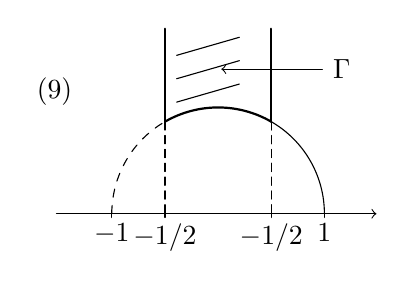
\begin{tikzpicture}[x=1.35cm,y=1.35cm,line cap=round]
\node[anchor=east] at (-1.28,1.15) {(9)};
\draw[->] (-1.52,0)--(1.49,0);
\draw[dashed] (-1,0) arc[start angle=180,end angle=120,radius=1];
\draw[thick] (-.5,.866) arc[start angle=120,end angle=60,radius=1];
\draw[thin] (.5,.866) arc[start angle=60,end angle=0,radius=1];
\draw[thick] (-.5,.866)--(-.5,1.74) (.5,.866)--(.5,1.74);
\draw[densely dashed] (-.5,.866)--(-.5,0) (.5,.866)--(.5,0);
\foreach \y in {1.05,1.27,1.49}{\draw (-.39,\y)--(.20,{\y+.17});}
\foreach \x in {-1,-.5,.5,1}
  {\draw (\x,.035)--(\x,-.035);}
\node[below] at (-1,0) {$-1$};
\node[below] at (-.5,0) {$-1/2$};
\node[below] at (.5,0) {$-1/2$};
\node[below] at (1,0) {$1$};
\draw[<-] (.03,1.36)--(.98,1.36);
\node[anchor=west] at (.99,1.36) {$\Gamma$};
\end{tikzpicture}}\endgroup}\par\smallskip}
\end{GelfandAdjacentEvidence}
\begin{GelfandAdjacentEvidence}{GELFAND-P001249}{9}

\EvidenceBlock{GELFAND-P001249}{axis-label}{Под правой вертикалью также написано \(-1/2\).}{Запись в рукописи.}
\end{GelfandAdjacentEvidence}
\begin{GelfandAdjacentEvidence}{GELFAND-P001249}{10}

$\triangle$ с углами \underline{$0^{\circ},60^{\circ},60^{\circ}$} на пл. Лобач.

Будем рассм. интегралы по $\triangle$-ку (9).

Выб. базис голом. квадр. дифф. на торе
\begin{equation*}
f^1=1,\qquad \eta_1=\frac{1}{\operatorname{Im}\tau}\tag{10}
\end{equation*}
\begin{equation*}
du=dz+\delta y^1\frac{d\bar z}{\operatorname{Im}\tau}
\end{equation*}
\Unclear{GELFAND-P001249}{du-overink}{После \(d\) перед знаком равенства буква густо обведена. Предположительно \(u\), возможно \(y\).}
\end{GelfandAdjacentEvidence}
\begin{GelfandAdjacentEvidence}{GELFAND-P001249}{11}

[Перед объяснением $u$ зачёркнуто.]
\Incomplete{GELFAND-P001249}{u-cancel-full}{неразборчивая зачёркнутая запись перед новым комплексным обозначением}
\end{GelfandAdjacentEvidence}

$u$ — нов. компл. коорд. (компл. структура)

$y^1$ — новая коорд. в пр-ве модулей.
\begin{equation*}
\text{Матр. содержит ровно 1 элемент:}\quad
\frac{dy^1\wedge d\bar y^1}{\operatorname{Im}\tau}\tag{11}
\end{equation*}


\Needspace{7\baselineskip}
\begin{GelfandAdjacentEvidence}{GELFAND-P001250}{1}
\SourcePage{GELFAND-P001250}{unlabelled}
\begin{equation*}
\tau\longrightarrow\frac{u(\tau)}{u(1)}
=\frac{\tau+\dfrac{\delta y^1\bar\tau}{\operatorname{Im}\tau}}
{1+\dfrac{\delta y^1}{\operatorname{Im}\tau}}\tag{12}
\end{equation*}
\begin{equation*}
u(z)=z+\frac{\delta y^1}{\operatorname{Im}\tau}\bar z\tag{13}
\end{equation*}
$y$ — координаты в пр-ве компл. структур

$y^1$ — любое, $\tau$ — вычисляется через $y^1$
\begin{equation*}
\frac{\overline{dy^1}\wedge dy^1}{\operatorname{Im}\tau}
=\frac{d\tau\wedge d\bar\tau}{4\operatorname{Im}\tau}
\end{equation*}
\EvidenceBlock{GELFAND-P001250}{wedge-order}{Слева дифференциал с чертой стоит первым, справа — вторым. В правом знаменателе перед \(\operatorname{Im}\tau\) написано \(4\).}{Запись в рукописи.}
\end{GelfandAdjacentEvidence}
\begin{GelfandAdjacentEvidence}{GELFAND-P001250}{2}


Теперь ост. вычислить:
\begin{equation*}
\int_{\Gamma}\frac{d\tau\wedge d\bar\tau}{\operatorname{Im}\tau}
\frac{\int\mathcal D X_{\mu}\,e^{\int X_{\mu}\partial\bar\partial X^{\mu}\,dz\wedge d\bar z}}
{\int\mathcal D\varepsilon\,e^{\int\bar\varepsilon\partial\bar\partial\varepsilon\,dz\wedge d\bar z}}\tag{14}
\end{equation*}
[Под формулой, стрелка вверх к мере интегрирования:] $\uparrow$ (Это не площадь! метрики).
И не удивит., т.к. начало не было инвар.

\begin{equation*}
X_{\mu}=a_{\mu}^n X^n_{\text{[\,\strut{}зач.\,]}},
\quad \Delta X^n_{\text{[\,\strut{}зач.\,]}}
=\lambda^n X^n_{\text{[\,\strut{}зач.\,]}}\tag{15}
\end{equation*}
\Incomplete{GELFAND-P001250}{eigen1-underink}{неразборчивый зачёркнутый нижний индекс у первого $X^n$}
\end{GelfandAdjacentEvidence}
\begin{GelfandAdjacentEvidence}{GELFAND-P001250}{3}

\Incomplete{GELFAND-P001250}{eigen2-underink}{неразборчивый зачёркнутый нижний индекс у второго $X^n$}
\end{GelfandAdjacentEvidence}
\begin{GelfandAdjacentEvidence}{GELFAND-P001250}{4}

\Incomplete{GELFAND-P001250}{eigen3-full}{неразборчивый зачёркнутый нижний индекс у третьего $X^n$}
\end{GelfandAdjacentEvidence}
\begin{GelfandAdjacentEvidence}{GELFAND-P001250}{5}

Получим
\begin{equation*}
\frac{\int dX_{\mu}^0(\det'\Delta)^{-13}}
{\int d\varepsilon^0(\det'\Delta)^{-1}}
=\frac{V}{\operatorname{Im}\tau}(\det'\Delta)^{-12}\tag{16}
\end{equation*}
[Зачёркнуто: Ко…]
\Incomplete{GELFAND-P001250}{cancel-word}{после «Ко» зачёркнуто и неразборчиво}
\end{GelfandAdjacentEvidence}
\begin{GelfandAdjacentEvidence}{GELFAND-P001250}{6}

Интегралы по 0-й моде остаются;

сверху — объём вселенной (26-мерной)

внизу — площадь тора

Положим $V=1$ временно.

Итог:
\begin{equation*}
-\int_{\Gamma}
\frac{d\tau\wedge d\bar\tau}
{(\operatorname{Im}\tau)^2}(\det'\Delta)^{-12}\tag{17}
\end{equation*}
\Unclear{GELFAND-P001250}{eq17-dtau}{В (17) верхний штрих первой \(\tau\) густо обведён. Неясно, есть ли над ней отдельная черта.}
\end{GelfandAdjacentEvidence}
\begin{GelfandAdjacentEvidence}{GELFAND-P001250}{7}

[Внизу:] (из м.(?) пар-ия) лишнее $\operatorname{Im}\tau$ $\Longrightarrow$ получилась площадь.
\Unclear{GELFAND-P001250}{bottom-abbrev}{Сокращение после «из» предположительно читается «м.». Начальные штрихи сливаются. Раскрытие сокращения неясно.}
\end{GelfandAdjacentEvidence}



\Needspace{7\baselineskip}
\begin{GelfandAdjacentEvidence}{GELFAND-P001251}{1}
\SourcePage{GELFAND-P001251}{59}
Как считать
\begin{equation*}
(\det'\Delta)^{-1/2}
=\int\mathcal D\psi\,e^{-\int\partial\psi\bar\partial\psi\,dz\wedge d\bar z}\tag{18}
\end{equation*}
Будем считать вариацию его $\ln$ по вар. компл. структуры.

$\Delta$ обычный — по компл. структуре!
\begin{equation*}
\delta\ln(\det'\Delta)^{-1/2}\tag{19}
\end{equation*}
Идея: базис, где диагонально и т.д.

\underline{Ответ:}
\begin{equation*}
\begin{aligned}
(\det'\Delta)^{-1/2}
&=(\operatorname{Im}\tau)^{-1/2}e^{\frac{\pi}{6}\operatorname{Im}\tau}
\prod_{n=1}^{\infty}\lvert1-e^{2\pi in\tau}\rvert^{-2}\\
&=(\operatorname{Im}\tau)^{-1/2}\lvert\eta(q)\rvert^{-2}
\end{aligned}\tag{20}
\end{equation*}
Для вычисления используем ф-лу (18)
\begin{equation*}
\delta(\ln\det^{-1/2}\Delta)
=\frac{\delta\int\mathcal D\psi\,e^{-\int\partial\psi\bar\partial\psi\,d^2\xi}}
{\int\mathcal D\psi\,e^{-\int\partial\psi\bar\partial\psi\,d^2\xi}}\tag{21}
\end{equation*}
[После дроби зачёркнуто.]
\Incomplete{GELFAND-P001251}{fraction-tail-cancel}{неразборчивая зачёркнутая группа после дроби (21)}
\end{GelfandAdjacentEvidence}
\begin{GelfandAdjacentEvidence}{GELFAND-P001251}{2}


При этом:

[Перед вариацией зачёркнуто.]
\Incomplete{GELFAND-P001251}{metric-before-cancel}{неразборчивая зачёркнутая группа перед вариацией метрики}
\end{GelfandAdjacentEvidence}
\begin{GelfandAdjacentEvidence}{GELFAND-P001251}{3}

\begin{equation*}
\delta(\sqrt g\,g^{ab}\partial_a\psi\partial_b\psi)=\delta g^{ab}T_{ab},
\end{equation*}
где
\begin{equation*}
T_{ab}=\partial_a\psi\partial_b\psi-\frac12g_{ab}\partial^a\psi\partial^b\psi
\end{equation*}
\Incomplete{GELFAND-P001251}{stress-lower-cancel}{зачёркнутый нижний индекс под верхним $a$ не читается}
\end{GelfandAdjacentEvidence}
\begin{GelfandAdjacentEvidence}{GELFAND-P001251}{4}

\EvidenceBlock{GELFAND-P001251}{stress-contraction}{В произведении после \(g_{ab}\) у производных написаны верхние индексы \(a\) и \(b\).}{Запись в рукописи.}
\end{GelfandAdjacentEvidence}
\begin{GelfandAdjacentEvidence}{GELFAND-P001251}{5}

\begin{equation*}
\delta g^{++}=\frac{\delta\tau}{\operatorname{Im}\tau},
\qquad \delta g^{--}=\frac{-\delta\bar\tau}{\operatorname{Im}\tau}
\qquad (?)
\end{equation*}
\Incomplete{GELFAND-P001251}{gpp-cancel-full}{зачёркнутый знак перед $\operatorname{Im}$ в знаменателе $\delta g^{++}$}
\end{GelfandAdjacentEvidence}
\begin{GelfandAdjacentEvidence}{GELFAND-P001251}{6}

\Incomplete{GELFAND-P001251}{gmm-cancel-full}{зачёркнутый знак перед $\operatorname{Im}$ в знаменателе $\delta g^{--}$}
\end{GelfandAdjacentEvidence}

Итого
\begin{equation*}
\delta(\ln\det^{-1/2}\Delta)
=2\operatorname{Re}\frac{i}{2}\delta\tau\langle T\rangle\tag{22}
\end{equation*}
здесь $T$ — тензор энергии–импульса,
\begin{equation*}
T(\xi)=\frac{\int\mathcal D\psi\,\partial\psi(\xi)\partial\psi(\xi)
e^{-\int\partial\psi\bar\partial\psi\,d^2\xi}}
{\int\mathcal D\psi\,e^{-\int\partial\psi\bar\partial\psi\,d^2\xi}}\tag{23}
\end{equation*}
Общая ф-ла (на пов. $\forall$ рода)
\begin{equation*}
\int d^2\xi\,(\eta T+\bar\eta\bar T).\tag{24}
\end{equation*}
[Справа, за двойной вертикальной чертой:] $\partial\bar T=\bar\partial T_{+-}$.

($T$ — почти голом. дифференциал)

Более аккур. запись (23): надо заменить $\partial\psi(\xi)\partial\psi(\xi)$ на $:\partial\psi(z)\partial\psi(z):$ и взять
\begin{equation*}
\begin{aligned}
T&=:\partial\psi(z)\partial\psi(z):
\overset{\mathrm{def}}{=}\oint\frac{dz'}{2\pi i}\frac{1}{z'-z}
\partial\psi(z')\partial\psi(z)\quad\overset{\text{или}}{=}\\
&=\langle\partial\psi(z)\partial\psi(z)\rangle
\overset{\mathrm{def}}{=}\biggl\langle\oint\frac{dz'}{2\pi i}\frac{1}{z'-z}
\partial\psi(z')\partial\psi(z)
\end{aligned}\tag{25}
\end{equation*}


\Needspace{7\baselineskip}
\begin{GelfandAdjacentEvidence}{GELFAND-P001252}{1}
\SourcePage{GELFAND-P001252}{unlabelled}
Формула для любого рода.

Есть $p$ штук аб. дифф. $\omega_i$ и координаты
\begin{equation*}
\vec z(Q)=\int_{Q_0}^{Q}\vec\omega\tag{26}
\end{equation*}
\begin{equation*}
\int_{b_i}\omega_j=\tau_{ij},\qquad
\int_{a_i}\omega_j=\delta_i^j\tag{27}
\end{equation*}
Введ. ещё $\theta$-ф-и:
\begin{equation*}
\theta_{\bar\varepsilon,\delta}(\vec z\mid\hat\tau)
=\sum_{\vec n}e^{\pi i\bigl(n_i\hat\tau_{ik}n_k
+2\pi i\vec z\cdot(\vec n+\vec\delta)}
\end{equation*}
\Incomplete{GELFAND-P001252}{theta-arg-cancel}{неразборчивый зачёркнутый знак после аргументов $\theta$}
\end{GelfandAdjacentEvidence}
\begin{GelfandAdjacentEvidence}{GELFAND-P001252}{2}

\Incomplete{GELFAND-P001252}{theta-exp-r2}{неразборчивый зачёркнутый знак после $n_i\hat\tau_{ik}n_k$ в первом показателе}
\end{GelfandAdjacentEvidence}
\begin{GelfandAdjacentEvidence}{GELFAND-P001252}{3}

\begin{equation*}
\sum_{\vec n}e^{\pi i(\vec n+\vec\delta,\hat\tau,\vec n+\vec\delta)
+2\pi i(\vec z+\vec\varepsilon)(\vec n+\vec\delta)}
\end{equation*}
\begin{equation*}
4\vec\delta\cdot\vec\varepsilon\pmod 2
\end{equation*}
\begin{equation*}
\theta^*\equiv\theta^{\bar\varepsilon,\bar\delta}_{,k}\omega_k(z);
\end{equation*}
[Стрелка к коэффициенту $\theta^{\bar\varepsilon,\bar\delta}_{,k}$:]
$\longleftarrow$ \underline{производная $\theta$ в нуле.}

[Справа:] $\bar\varepsilon,\bar\delta$ — нечетная хар-ка.

из этого аб. дифф. можно извлечь корень (все нули — 2-го пор.).
\begin{equation*}
T=\frac12
\underbrace{\left[\frac{\theta^{*''}}{\theta^*}
-\frac32\left(\frac{\theta^{*'}}{\theta^*}\right)^2\right]}_{\text{шварциан}}
-\frac16\frac{\theta_{,ijk}\omega_i\omega_j\omega_k}{\theta'}
-\frac\pi2\omega_i(\operatorname{Im}\hat\tau)^{-1}_{ik}\omega_k
\tag{28}
\end{equation*}
\EvidenceBlock{GELFAND-P001252}{theta-stress-formula}{В первом числителе написано \(\theta^{*''}\), в знаменателе следующей дроби — \(\theta'\).}{Запись в рукописи.}
\end{GelfandAdjacentEvidence}


Всё это вместе — квадратичный дифференциал.

$\omega$ не сод. $dz$: $\omega_i\,dz$ — форма.


\clearpage
\pdfbookmark[0]{Глава 28}{gelfand-archive-chapter-28}
\section*{Глава 28}
\Needspace{7\baselineskip}
\begin{GelfandAdjacentEvidence}{GELFAND-P001253}{1}
\SourcePage{GELFAND-P001253}{unlabelled}
\underline{\underline{17/II — 86 г.}}\qquad\underline{Сем. Гельфанда.}

\underline{\underline{Бейлинсон А.}}\qquad [Зачёркнуто: О теории(?)] \underline{Детерминант Квиллена, струны и пр.}
\Unclear{GELFAND-P001253}{title-cancel}{возможно «О теории»}
\end{GelfandAdjacentEvidence}
\begin{GelfandAdjacentEvidence}{GELFAND-P001253}{2}


Вычисляем статсумму
\begin{equation*}
Z=\sum_{p\geq0}Z_p.\tag{1}
\end{equation*}
$p$ — род
\begin{equation*}
Z_p=\int_{M_p}\mu_p,\qquad
\begin{aligned}
M_p&\text{ — пр-во модулей кривых рода }p.\\
\mu_p&\text{ — естеств. возник. мера}
\end{aligned}\tag{2}
\end{equation*}
При $p=1$ независимо вычислили Кронекер (1890) и Шапиро (1972) (одинаково)
\begin{equation*}
\mu_1=\left|\frac{dq}{q}\right|^2\Delta(q)^{-2}\log|q|^{-13},
\qquad \Delta(q)=q\prod(1-q^n)^{24}.\tag{3}
\end{equation*}
\Unclear{GELFAND-P001253}{log-exponent}{В (3) виден показатель \(-13\). Над ним приписано \(13\) с направленной к показателю стрелкой. Затёртые штрихи показателя и запись в скобках после приписки неразборчивы.}
\end{GelfandAdjacentEvidence}


$\mu_1$ — мера на пр-ве модулей элл. кривых

\begin{center}— . —\end{center}
$X$ — пов. рода $p$; $g$ — метрика на $X$;
$L$ — одномерное голом. рассл. на $X$
(голом. структ., индуц. метрикой), $h$ — эрмитова метрика на $L$
\begin{equation*}
\bar\partial:\Gamma(L)\longrightarrow\Gamma(L\otimes\Omega^{0,1}).\tag{4}
\end{equation*}
Тогда
\begin{equation*}
\underset{\substack{|\\\text{голом. сечения}}}{H^0(X,L)}
=\operatorname{Ker}\bar\partial,\qquad
H^1(X,L)=\operatorname{Coker}\bar\partial=\operatorname{Ker}\bar\partial^{+}.
\tag{5}
\end{equation*}
(Голом. рассл. описываются одним дискр. пар. — числом Черна и $p$ непрерывными пар. — точка на якобиане)

$H^0$, $H^1$ конечномерны
\begin{equation*}
d(X,L):=\frac{\det H^0(X,L)}{\det H^1(X,L)}.\tag{6}
\end{equation*}
$\det H^0=\max$ внешн. степень $H^0$ — одномерное вект. пр-во

[Следующая строка обозначена длинными чертами и знаком повтора; в ней вместо $H^0$ стоит $H^1$.]

Поэтому $d(X,L)$ — тоже 1-мерное вект. пр-во.

(ф-ии на $\det H^1$ со знач. в $\det H^0$)

На нём есть естеств. метрика
\begin{equation*}
\begin{array}{l|l}
e_1,\ldots,e_k\text{ — базис в }H^0&
\displaystyle d(X,L)\ni
\underset{\substack{\uparrow\\\mathbb C}}{\lambda}
\frac{e_1\wedge\cdots\wedge e_k}{g_1\wedge\cdots\wedge g_d}\\
g_1,\ldots,g_d\text{ — базис в }H^1&
\end{array}
\end{equation*}


\Needspace{7\baselineskip}
\begin{GelfandAdjacentEvidence}{GELFAND-P001254}{1}
\SourcePage{GELFAND-P001254}{4}
Метрика будет опр. в 2 этапа.

Сначала \underline{глупая} метрика. Рассм. [вписано сверху: естеств.] метрику на
\Unclear{GELFAND-P001254}{top-cancel}{Зачёркнутое сокращение предположительно читается «пр.».}
\end{GelfandAdjacentEvidence}
\begin{GelfandAdjacentEvidence}{GELFAND-P001254}{2}

$\Gamma(L)$ и на $\Omega^{0,1}$,
определяющие там предгильбертовы структуры.

На $H^0$ и $H^1=\operatorname{Ker}\bar\partial^{+}$ тоже индуцируются метрики
$\Rightarrow$\newline
$\Rightarrow$ возникает метрика в $d(X,L)$, называемая глупой.

[Вписано сверху: Построим] \underline{правильную метрику.}
[Слева стрелка вниз.]

Рассм. $\Delta=\bar\partial^{+}\bar\partial$ и его $\det\Delta$, вычисленный Белавиным и Книжником;

$\Delta'$ — тот же $\Delta$, но с выброшенными нулевыми модами.
\begin{equation*}
\det\Delta'=\exp\bigl(-\zeta'_{\Delta'}(0)\bigr),
\end{equation*}
\begin{equation*}
\zeta_{\Delta'}(s)=
\sum_{\substack{\lambda\in\text{соб. зн.}\,\Delta,\\\lambda\ne0}}
\lambda^{-s},\qquad\operatorname{Re}s>1
\end{equation*}
\begin{equation*}
\begin{aligned}
&\underline{\text{Метрика Квиллена на }d(X,L)}
\quad\left(\substack{\text{из статьи в ФА}\\1985,\ N=1\ (?) }\right)\\
&\hspace{1em}=(\text{глупая метрика})\cdot\sqrt{\det\Delta'}.
\end{aligned}\tag{7}
\end{equation*}
\EvidenceBlock{GELFAND-P001254}{quillen-issue}{В рукописи написано \(N=1\ (?)\) со знаком вопроса в скобках.}{Запись в рукописи.}
\end{GelfandAdjacentEvidence}
\begin{GelfandAdjacentEvidence}{GELFAND-P001254}{3}


\underline{Пояснение к определению (7).} Пусть
\begin{equation*}
E_1\xrightarrow{\bar\partial}E_2
\quad\text{— пр-ва с метрикой (конечномерные)}\tag{8}
\end{equation*}
\begin{equation*}
d=\frac{\det\operatorname{Ker}\bar\partial}{\det\operatorname{Coker}\bar\partial}
\underset{\substack{\uparrow\\\text{каноническое}\\\text{отождествление}}}{=}
\frac{\det E_1}{\det E_2}.\tag{9}
\end{equation*}
Пусть даны базисы.\qquad Причём предположим, что
\begin{equation*}
\begin{array}{l|l}
e_1,\ldots,e_k\text{ — базис в }E_1&
\underbrace{e_1,\ldots,e_a}_{\text{базис в }\operatorname{Ker}\bar\partial}\\[2pt]
g_1,\ldots,g_{\ell}\text{ — — '' — }E_2&g_{a+1},\ldots,g_k\\
&g_{a+1}=\bar\partial e_{a+1},\ldots,g_k=\bar\partial e_k.
\end{array}\tag{10}
\end{equation*}
и
\Unclear{GELFAND-P001254}{corrected-bases}{Зачёркнуто \(e_1\wedge\cdots\wedge e_a\). Перед ним зачёркнуты неразборчивые слова. Над следующей строкой вписано «соотв.». Прежние штрихи над «базисов» неразборчивы.}
\end{GelfandAdjacentEvidence}
\begin{GelfandAdjacentEvidence}{GELFAND-P001254}{4}

отношения [вписано: соотв.] базисов в (9) друг другу соответствуют.

Есть метрики справа и слева в (9); они не совпадают — [зачёркнуто: разница; вписано: отлич.] множителем $\sqrt{\det\Delta}$

Слева — глупая, справа — та, к-рая нам нужна, но теперь мы определяем
\Unclear{GELFAND-P001254}{bottom-cancel}{Под косыми штрихами зачёркивания предположительно читается «её».}
\end{GelfandAdjacentEvidence}

правую часть по левой в $\infty$-мерной ситуации.


\Needspace{7\baselineskip}
\begin{GelfandAdjacentEvidence}{GELFAND-P001255}{1}
\SourcePage{GELFAND-P001255}{unlabelled}
Естественность «правильной» метрики: она \underline{не меняется при вариации оператора $\bar\partial$}.

В (9) если $\operatorname{Ker}\bar\partial=\operatorname{Coker}\bar\partial=0$
стоит справа $\det\bar\partial$
\begin{equation*}
\text{Вообще}\quad
\det(\bar\partial:E_1\to E_2)\in\frac{E_1}{E_2}
\quad\text{для одномерных }E_1,E_2.
\end{equation*}
\EvidenceBlock{GELFAND-P001255}{determinant-quotient}{В числителе \(E_1\), в знаменателе \(E_2\).}{Запись в рукописи.}
\end{GelfandAdjacentEvidence}
\begin{GelfandAdjacentEvidence}{GELFAND-P001255}{2}

В $\infty$-мерн. случае есть только модуль прав. части (9)

\underline{Недостижимый идеал:} определить прав. часть в (9) независимо
\Unclear{GELFAND-P001255}{functor-cancel}{Короткий зачёркнутый фрагмент неразборчив.}
\end{GelfandAdjacentEvidence}
\begin{GelfandAdjacentEvidence}{GELFAND-P001255}{3}

от $\bar\partial$, чтобы было функториально (изом. пр-в $\Rightarrow$ изом. $\det$)

Пусть $L$ — рассл. $j$-дифференциалов, $L=\omega^j$,
его сеч. $f(z)(dz)^j$.
\begin{equation*}
\begin{aligned}
&\underset{\substack{\Vert\\\rho\,dz\,d\bar z}}{\text{Рим. метрика}}
\quad\text{[зачёркнутая вставка: на $L$]}\\
&\qquad\text{индуцирует метрику на }\omega^j
\quad\Rightarrow\quad \lvert(dz)^j\rvert^2=\rho^{-j}.
\end{aligned}\tag{11}
\end{equation*}
\Unclear{GELFAND-P001255}{power-cancel}{После $-j$ зачёркнуты неразборчивые знаки.}
\end{GelfandAdjacentEvidence}
\begin{GelfandAdjacentEvidence}{GELFAND-P001255}{4}

Здесь $j\in\mathbb Z$.

Пр-во $d(x,\omega^j)$ зав. только от компл. структуры на $X$.

Метрика $\lvert\ \rvert_j\bigl(\underset{\substack{\vert\\\text{метрика на $X$}}}{\rho}\bigr)$
— метрика Квиллена на $d(X,\omega^j)$

\noindent (12) \underline{Теорема} (Поляков)
\Unclear{GELFAND-P001255}{theorem-cancel}{Зачёркнутое сокращение предположительно читается «Рассм.».}
\end{GelfandAdjacentEvidence}
\begin{GelfandAdjacentEvidence}{GELFAND-P001255}{5}

\begin{equation*}
\frac{\delta\bigl(\log\lvert\ \rvert_j(\rho)\bigr)}{\delta\rho}
=(6j^2-6j+1)\underset{\substack{\vert\\\text{кривизна метрики}}}{R(\rho)}
\end{equation*}

\noindent (13) Обозначение: $c_j=6j^2-6j+1$
\qquad (2-й многочлен Бернулли)

\noindent (14) \underline{Следствие}.
Пусть дан набор $j_1,\ldots,j_a\in\mathbb Z$,
[вставка сверху: и целые $b_1,\ldots,b_a\in\mathbb Z$,]
такой что $\sum_{k=1}^{a}b_kc_{j_k}=0$.
\Unclear{GELFAND-P001255}{sum-overwrite}{Нижний индекс при \(b\) затёрт. Индекс суммы \(k\) и соседний множитель \(c_{j_k}\) поддерживают чтение \(b_k\).}
\end{GelfandAdjacentEvidence}
\begin{GelfandAdjacentEvidence}{GELFAND-P001255}{6}


Рассм. метрику Квиллена на $\otimes\,d(X,\omega^{j_k})^{b_k}$.
\Unclear{GELFAND-P001255}{tensor-cancel}{Короткий зачёркнутый фрагмент неразборчив.}
\end{GelfandAdjacentEvidence}
\begin{GelfandAdjacentEvidence}{GELFAND-P001255}{7}

Тогда она не зависит от [вписано: исходной] $\rho$,
а зав. лишь от компл. структуры на $X$

\noindent (15) \underline{Опр.} $c_j$ наз. \underline{конформной аномалией}.

\noindent (16) \underline{Важнейший пример}.
\begin{equation*}
\begin{aligned}
j_1&=2,&b_1&=1,\\
j_2&=1,&b_2&=-13
\end{aligned}
\qquad\text{— соотв. число }\underline{\underline{13}}
\end{equation*}
\Unclear{GELFAND-P001255}{coefficient-correction}{У $b_2$ после минуса прежняя запись затёрта. Сверху вписано $13$.}
\end{GelfandAdjacentEvidence}


(В 26-мерн. пр-ве нет конф. аномалии)
\begin{center}— . —\end{center}


\Needspace{7\baselineskip}
\begin{GelfandAdjacentEvidence}{GELFAND-P001256}{1}
\SourcePage{GELFAND-P001256}{5}
\SourceFigure{GELFAND-P001256}{family-arrow}{%
\par\smallskip
{\color{black}\begingroup\color{black}\GelfandFitDiagram{\begin{tikzpicture}[x=1cm,y=1cm]
\node[anchor=east] at (-.35,0) {(17)};
\node (total) at (0,.55) {$X_M$};
\node (base) at (0,-.55) {$M$};
\draw[->] (total)--(base);
\node[anchor=west,align=left] at (.5,0) {[вставка: голом.] сем-во кривых\\($M$ — база деформаций)};
\end{tikzpicture}}\endgroup}\par\smallskip}
\end{GelfandAdjacentEvidence}
\begin{GelfandAdjacentEvidence}{GELFAND-P001256}{2}


Тогда $\forall$ целого $j$ возникает 1-мерное рассл. $d_j$ над $M$
со слоем $d(X_t,\omega^j)$ над $t\in M$.

Это
\Unclear{GELFAND-P001256}{top-cancel}{Зачёркнуто: вероятно «есть».}
\end{GelfandAdjacentEvidence}
\begin{GelfandAdjacentEvidence}{GELFAND-P001256}{3}

одномерное голом. расслоение над $M$.

\noindent (18)
\Unclear{GELFAND-P001256}{eq18-cancel}{Зачёркнуто: возможно «На».}
\end{GelfandAdjacentEvidence}
\begin{GelfandAdjacentEvidence}{GELFAND-P001256}{4}

над $\otimes\,d(X_t,\omega^{j_i})^{b_{j_i}}$ имеется кан. эрм. метрика
($b_j$ как в (14))
\EvidenceBlock{GELFAND-P001256}{eq18-index}{В (18) показатель записан с составным нижним индексом \(b_{j_i}\).}{Запись в рукописи.}
\end{GelfandAdjacentEvidence}
\begin{GelfandAdjacentEvidence}{GELFAND-P001256}{5}


\noindent (19) \underline{Теорема} (Белавин, Книжник):

\underline{Кривизна кан. метрики на} $\otimes\,d(X,\omega^{j_i})^{b_i}$ равна 0.

\underline{Слова:} из уничт. конф. аномалии вытек. уничт. гравитационной.

Теорема (19) однозначно опр. [вставка: кан.] метрику (к-рая будет опр. только родом)
\EvidenceBlock{GELFAND-P001256}{metric-uniqueness}{В рукописи «Теорема (19) однозначно опр. [вписано: кан.] метрику».}{Запись в рукописи.}
\end{GelfandAdjacentEvidence}
\begin{GelfandAdjacentEvidence}{GELFAND-P001256}{6}


\underline{\underline{Белавин}}
\begin{equation*}
\begin{aligned}
\sum_{\text{поверхн.}}e^{-a(\text{площадь})}
&=\sum_{p=2}^{\infty}\int d\mu_0^{(p)}
\frac{\det\Delta_{-1}^{(p)}}{(\det\Delta_0^{(p)})^{13}}\\[-1pt]
&\hspace{2em}(\text{Поляков $+$ уточнения для произв. рода})
\end{aligned}\tag{20}
\end{equation*}
$\Delta_j$ — лапл. на $j$-формах

Важно: справа —
\SourceFigure{GELFAND-P001256}{eq20-arrow}{%
\par\smallskip
{\color{black}\begingroup\color{black}\GelfandFitDiagram{\begin{tikzpicture}[x=1cm,y=1cm]
\node (fraction) at (0,1.55) {$\underbrace{\dfrac{\det\Delta_{-1}^{(p)}}{(\det\Delta_0^{(p)})^{13}}}$};
\node[draw,align=center,inner sep=4pt] (modulus) at (0,-.15) {кв. модуля голом. ф-и\\на пр-ве модулей};
\node[align=center] (unique) at (0,-1.45) {уже [вставка: почти] однозначно};
\draw[->] (modulus.north)--(fraction.south);
\draw[->] (modulus.south)--(unique.north);
\end{tikzpicture}}\endgroup}\par\smallskip}
\end{GelfandAdjacentEvidence}
\begin{GelfandAdjacentEvidence}{GELFAND-P001256}{7}


\begin{equation*}
\delta\bar\delta\log\det\Delta_j
=c_j\int\frac{\partial f\,\bar\partial\bar f
-f\bar f\,\partial\bar\partial\log\rho}{\rho^2},
\qquad f=\rho\eta,\tag{21}
\end{equation*}
\begin{equation*}
\delta_{\rho}\log\det\Delta_j=c_jR
\qquad\text{Вар. метрики: }dz\,d\bar z\longrightarrow\lvert dz+\eta\,d\bar z\rvert^2
\tag{21'}
\end{equation*}
\Unclear{GELFAND-P001256}{variation-cancel}{Над $d\bar z$ слева от стрелки зачёркнуты неразборчивые знаки.}
\end{GelfandAdjacentEvidence}
\begin{GelfandAdjacentEvidence}{GELFAND-P001256}{8}


\underline{Бейлинсон}

Интеграл в (20) расходится и его ещё надо перенормировать.

\underline{Белавин}
\begin{equation*}
Z_1=\int\frac{d\tau\,d\bar\tau}{(\operatorname{Im}\tau)^2}
\cdot\frac{1}{(\operatorname{Im}\tau)^{12}}\cdot\frac{1}{\lvert\Delta(q)\rvert^2},
\qquad q=e^{2\pi i\tau}
\end{equation*}
\Unclear{GELFAND-P001256}{z1-cancel}{После $(\operatorname{Im}\tau)^2$ в первом знаменателе зачёркнут неразборчивый знак.}
\end{GelfandAdjacentEvidence}

Инт. расходится.

Но есть гипотеза, что в суперструне всё сходится.
\begin{equation*}
Z_2=\int\frac{d^2\tau}{(\operatorname{Im}\tau)^3}
\cdot\frac{1}{(\operatorname{Im}\tau)^{10}}\cdot\frac{1}{\lvert F(\tau)\rvert^2},
\qquad
\tau=\begin{bmatrix}\tau_{11}&\tau_{12}\\\tau_{21}&\tau_{22}\end{bmatrix}
\end{equation*}
$\tau$ — матр. периодов

(Книжник, Морозов, Переломов)
\begin{equation*}
F(\tau)=\prod\theta_m^2(\tau)
\end{equation*}
$Z_3$ тоже есть.

Для общего $p$ нет хорошего опис. пр-ва модулей.


\Needspace{7\baselineskip}
\begin{GelfandAdjacentEvidence}{GELFAND-P001257}{1}
\SourcePage{GELFAND-P001257}{unlabelled}
\underline{Бейлинсон}

$M$ — пр-во модулей;
\[
p>2\Rightarrow\forall\ \underline{\text{голом. ф-я}}=\mathrm{const}
\]

Метрика [вставка сверху: 0-й кривизны] опр. с точн. до квадр. модуля
\Unclear{GELFAND-P001257}{cancelled-word}{Под зачёркиванием предположительно читается сокращение «функц.».}
\end{GelfandAdjacentEvidence}
\begin{GelfandAdjacentEvidence}{GELFAND-P001257}{2}

голом. ф-и $\Rightarrow$ тем самым однозначно.
Остаётся её вычислить. (Свод. к вычислению единственного голом. сечения
\Unclear{GELFAND-P001257}{last-line-overwrite}{Под «голом.» затёртая короткая отметка, чтение не установлено.}
\end{GelfandAdjacentEvidence}

нек-рого расслоения).


\Needspace{7\baselineskip}
\begin{GelfandAdjacentEvidence}{GELFAND-P001258}{1}
\SourcePage{GELFAND-P001258}{unlabelled}
\underline{24/II-85.}\qquad
\underline{\underline{Концевич}} (\underline{Максим}) (сем. Гельфанда)
\Unclear{GELFAND-P001258}{date-conflict}{В рукописи «24/II-85.». Каталог, запись 667, датирует доклад 24 февраля 1987 г.}
\end{GelfandAdjacentEvidence}
\begin{GelfandAdjacentEvidence}{GELFAND-P001258}{2}


\Unclear{GELFAND-P001258}{heading-cancel}{В зачёркнутой строке читаются \(\widetilde M_g\) и «пр-во бесконечномер…». Конец слова затёрт.}
\end{GelfandAdjacentEvidence}
\begin{GelfandAdjacentEvidence}{GELFAND-P001258}{3}

$M_g$ — пр-во
\Unclear{GELFAND-P001258}{moduli-cancel}{Зачёркнутое слово предположительно читается «Модулей».}
\end{GelfandAdjacentEvidence}
\begin{GelfandAdjacentEvidence}{GELFAND-P001258}{4}

Тейхмюлера
\begin{equation*}
(\text{Кривая }C,\ \text{точка }p\in C,\ x\text{ — коорд. в }p)
=\widetilde M_g
\end{equation*}
\begin{equation*}
\begin{gathered}
\mathfrak g=\mathbb C((x))\frac{\partial}{\partial x}\\
\cup\\
\mathfrak k=\mathbb C[[x]]\frac{\partial}{\partial x}
\end{gathered}
\qquad
\begin{gathered}
\gamma\text{ — ряды Лорана вект. полей на }C\\
\text{с полюсом в }p.\\
\gamma\subset\mathfrak g
\end{gathered}
\end{equation*}
\Unclear{GELFAND-P001258}{gamma-correction}{Первый знак $\gamma$ обведён и затёрт. Ниже он повторяется разборчиво.}
\end{GelfandAdjacentEvidence}
\begin{GelfandAdjacentEvidence}{GELFAND-P001258}{5}

\Unclear{GELFAND-P001258}{pole-correction}{Окончание в слове «полюсом» обведено и затёрто. Сходный оборот ниже поддерживает это чтение.}
\end{GelfandAdjacentEvidence}
\begin{GelfandAdjacentEvidence}{GELFAND-P001258}{6}

$\widetilde M_g$ в окр. точки — однор. пр-во $\mathfrak g/\gamma$

\noindent (1) \underline{Теор. 1.} На $\widetilde M_g$ действует $\mathfrak g$,
стабилизатор точки [вставка сверху: $t$] есть \(\gamma\)

опис. действия $\mathfrak g$ на $\widetilde M_g$

Пусть дано однопар. сем-во кривых; на этом нелин. рассл. есть связность с полюсом лишь в т. $p$.
\SourceFigure{GELFAND-P001258}{family-sketch}{%
\par\smallskip
{\color{black}\begingroup\color{black}\GelfandFitDiagram{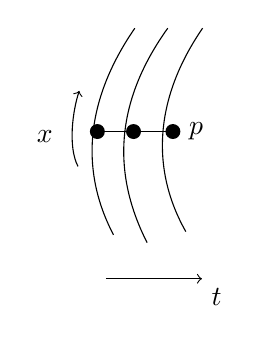
\begin{tikzpicture}[x=.82cm,y=.82cm]
\draw (0.35,0) .. controls (-0.20,1.05) and (-0.05,2.14) .. (0.68,3.2);
\draw (0.87,-0.12) .. controls (0.28,1.04) and (0.43,2.14) .. (1.19,3.2);
\draw (1.47,0.05) .. controls (0.91,1.04) and (1.00,2.14) .. (1.73,3.2);
\draw (0.10,1.60)--(1.27,1.60);
\fill (0.10,1.60) circle (2.7pt);
\fill (0.66,1.60) circle (2.7pt);
\fill (1.27,1.60) circle (2.7pt);
\node[right] at (1.37,1.60) {$p$};
\draw[->] (-.20,1.06) .. controls (-.36,1.37) and (-.28,1.93) .. (-.18,2.23);
\node[left] at (-.44,1.53) {$x$};
\draw[->] (.23,-.68)--(1.72,-.68);
\node[below right] at (1.72,-.68) {$t$};
\end{tikzpicture}}\endgroup}\par\smallskip}
\end{GelfandAdjacentEvidence}
\begin{GelfandAdjacentEvidence}{GELFAND-P001258}{7}

\begin{equation*}
\nabla_t=\frac{\partial}{\partial t}+F(x,t)\frac{\partial}{\partial x}
\end{equation*}
Кас. пр-во к $\widetilde M_g$ отожд. с $\mathfrak g/\mathfrak k$.
\EvidenceBlock{GELFAND-P001258}{tangent-quotient}{В строке о касательном пространстве написано \(\mathfrak g/\mathfrak k\).}{Запись в рукописи.}
\end{GelfandAdjacentEvidence}
\begin{GelfandAdjacentEvidence}{GELFAND-P001258}{8}

\begin{equation*}
\begin{aligned}
T(\widetilde M_g)_{(C,x,p)}
&\underset{\substack{\uparrow\\\text{изоморфизм}\\\text{Кодаира—Спенсера}}}{=}
\mathbb C((x))\frac{\partial}{\partial x}\big/\\[-2pt]
&\hspace{4em}\text{вект. поля, продолж. на }C\setminus\{p\}
\end{aligned}
\end{equation*}
\begin{flushright}[На полях: (всю $C$!!)]\end{flushright}
\Unclear{GELFAND-P001258}{coordinate-corrections}{Буква $x$ в ряде и в знаменателе производной обведена. Прежние штрихи неразборчивы.}
\end{GelfandAdjacentEvidence}
\begin{GelfandAdjacentEvidence}{GELFAND-P001258}{9}


$\widetilde{\mathfrak g}$ — алг. Вирасоро.
Она действует
\Unclear{GELFAND-P001258}{action-cancel}{Зачёркнуто «в» и \(M\) с тильдой. Нижний индекс затёрт, предположительно \(g\).}
\end{GelfandAdjacentEvidence}
\begin{GelfandAdjacentEvidence}{GELFAND-P001258}{10}

в расслоении $d_k$.
\SourceFigure{GELFAND-P001258}{lift-arrow}{%
\par\smallskip
{\color{black}\begingroup\color{black}\GelfandFitDiagram{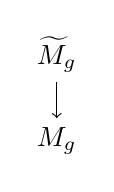
\begin{tikzpicture}[x=1cm,y=1cm]
\node (upper) at (0,.55) {$\widetilde M_g$};
\node (lower) at (0,-.55) {$M_g$};
\draw[->] (upper)--(lower);
\end{tikzpicture}}\endgroup}\par\smallskip}
\end{GelfandAdjacentEvidence}

$d_k$ — дет. расслоение над $M_g$, поднятое на $\widetilde M_g$


\Needspace{7\baselineskip}
\begin{GelfandAdjacentEvidence}{GELFAND-P001259}{1}
\SourcePage{GELFAND-P001259}{unlabelled}
\underline{24.2.86.}\qquad\underline{Сем. Гельфанда}

\underline{\underline{Морозов}}\qquad
\underline{Следствия теор. Белавина—Книжника.}
\Unclear{GELFAND-P001259}{date-conflict}{В рукописи «24.2.86.». Каталог, запись 668, датирует доклад 24 февраля 1987 г.}
\end{GelfandAdjacentEvidence}
\begin{GelfandAdjacentEvidence}{GELFAND-P001259}{2}


Явные ф-лы для бозонных струн и т.д.

Бозонная струна в крит. разм. $d=26$.

Резюме докл. Бейлинсона:
\EvidenceBlock{GELFAND-P001259}{continuation-note}{Первое слово читается «Резюме». Его пересекают штрихи верхней строки.}{Запись в рукописи.}
\end{GelfandAdjacentEvidence}
\begin{GelfandAdjacentEvidence}{GELFAND-P001259}{3}

\begin{equation*}
\begin{aligned}
&\sum_p\int Dx\,Dg\ \exp\int\sqrt g\,g^{ab}\partial_a x^\mu\partial_b x^\mu\,d^2\xi\prod_\alpha V_\alpha={}\\
&\qquad=\sum_p\int_{M_p}\frac{\lvert d\mu_p\rvert^2}{(\det\operatorname{Im}T)^{13}}\ K\{V\}
\end{aligned}\tag{1}
\end{equation*}
\EvidenceBlock{GELFAND-P001259}{det-exponent}{Густо обведённый показатель читается \(13\).}{Запись в рукописи.}
\end{GelfandAdjacentEvidence}
\begin{GelfandAdjacentEvidence}{GELFAND-P001259}{4}

$V_\alpha$ — вершинные операторы (потом будет пояснено)

\SourceFigure{GELFAND-P001259}{tube-diagram}{%
\par\smallskip
{\color{black}\begingroup\color{black}\GelfandFitDiagram{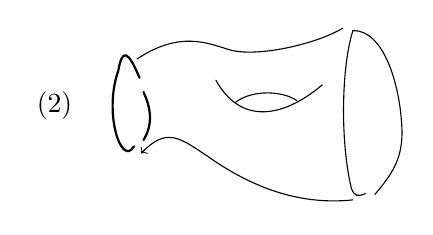
\begin{tikzpicture}[x=1cm,y=1cm,line cap=round]
\node[anchor=east] at (-.48,.12) {(2)};
\draw[thick] (.25,.47) .. controls (.10,.83) and (.03,.84) .. (-.02,.56)
  .. controls (-.21,.02) and (.02,-.67) .. (.18,-.40);
\draw[thick] (.30,.29) .. controls (.40,.08) and (.42,-.13) .. (.30,-.32);
\draw (.22,.71) .. controls (.76,1.07) and (1.12,.91) .. (1.38,.83)
  .. controls (1.73,.72) and (2.50,.90) .. (2.83,1.10);
\draw[->] (2.96,-1.08) .. controls (2.21,-1.16) and (1.59,-.86) .. (1.12,-.53)
  .. controls (.75,-.28) and (.59,-.16) .. (.27,-.49);
\draw (2.96,1.07) .. controls (2.81,.59) and (2.80,-.35) .. (2.94,-.93)
  .. controls (2.98,-1.04) and (3.02,-1.04) .. (3.12,-1.00);
\draw (2.96,1.07) .. controls (3.34,1.08) and (3.55,.42) .. (3.58,-.13)
  .. controls (3.61,-.55) and (3.45,-.76) .. (3.24,-1.01);
\draw (1.22,.44) .. controls (1.53,-.12) and (2.06,-.05) .. (2.57,.38);
\draw (1.47,.16) .. controls (1.68,.32) and (2.06,.31) .. (2.25,.18);
\end{tikzpicture}}\endgroup}\par\smallskip}
\end{GelfandAdjacentEvidence}
\begin{GelfandAdjacentEvidence}{GELFAND-P001259}{5}

\underline{мировая пов. распр. колечка}
\Unclear{GELFAND-P001259}{tube-caption}{В подписи написано сокращение «распр.». Раскрытие сокращения не указано.}
\end{GelfandAdjacentEvidence}
\begin{GelfandAdjacentEvidence}{GELFAND-P001259}{6}


Взаимные превр. учитываются рассмотрением разн. топологий.

Технич. удобно счит. в нач. и в конце — точки.

\SourceFigure{GELFAND-P001259}{point-diagram}{%
\par\smallskip
{\color{black}\begingroup\color{black}\GelfandFitDiagram{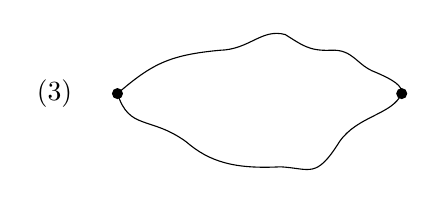
\begin{tikzpicture}[x=1cm,y=1cm,line cap=round]
\node[anchor=east] at (-.45,0) {(3)};
\draw (0,0) .. controls (.43,.37) and (.65,.49) .. (1.30,.55)
  .. controls (1.68,.56) and (1.83,.83) .. (2.13,.75)
  .. controls (2.34,.62) and (2.43,.54) .. (2.70,.55)
  .. controls (3.00,.57) and (3.03,.36) .. (3.28,.27)
  .. controls (3.51,.17) and (3.62,.10) .. (3.61,0)
  .. controls (3.49,-.27) and (3.05,-.28) .. (2.82,-.61)
  .. controls (2.52,-1.09) and (2.45,-.95) .. (2.07,-.93)
  .. controls (1.49,-.96) and (1.17,-.87) .. (.87,-.61)
  .. controls (.41,-.28) and (.15,-.47) .. (0,0);
\fill (0,0) circle (2pt);
\fill (3.61,0) circle (2pt);
\end{tikzpicture}}\endgroup}\par\smallskip}
\end{GelfandAdjacentEvidence}
\begin{GelfandAdjacentEvidence}{GELFAND-P001259}{7}

Тогда $V_\alpha$ — $\delta$-ф-и; переходя к пр. Фурье, получим
($\alpha$ — номер верш. опер.)
\begin{equation*}
V_\alpha(p)=\int e^{i p_\alpha x(\xi)}d^2\xi
\tag{4}
\end{equation*}
\Unclear{GELFAND-P001259}{eq4-cancel}{После $p_\alpha$ в показателе зачёркнут неразборчивый знак, возможно $\mu$.}
\end{GelfandAdjacentEvidence}
\begin{GelfandAdjacentEvidence}{GELFAND-P001259}{8}


Удобно брать и производные $\delta$-ф-й:
\begin{equation*}
V_\alpha(p)=\int\partial x^\mu(\xi)e^{i p_\alpha x(\xi)}d^2\xi
\tag{4'}
\end{equation*}

Для получ. прав. части в (1):

а) Интегрируем по $x$, получим
\begin{equation*}
\frac{1}{(\det\Delta_0)^{13}}\prod_\alpha\int d^2\xi_\alpha
\prod_{\alpha,\beta}\exp p_\alpha p_\beta\,G_{(reg)}(\xi_\alpha,\xi_\beta)
\tag{5}
\end{equation*}
$\Delta_0$ — лапласиан на скалярах

$G_{(reg)}$ — рег. ф-я Грина (сглаж., когда точки совпадают)

\Unclear{GELFAND-P001259}{right-edge-traces}{На правом поле видны слабые изогнутые штрихи. Чтение не установлено.}
\end{GelfandAdjacentEvidence}



\Needspace{7\baselineskip}
\begin{GelfandAdjacentEvidence}{GELFAND-P001260}{1}
